\documentclass[11pt]{extarticle}

\usepackage{color}
\usepackage{graphicx}
\usepackage{fullpage}
\usepackage{verbatim}
\usepackage{tikz}
\usepackage{listings}
\usepackage[yyyymmdd,hhmmss]{datetime}
\usepackage{rotating}
\usepackage{authblk}
\usepackage{amsfonts}
\usepackage{todonotes}
\usepackage{titlesec}
\usepackage{lineno}
\usepackage{tabularx}
\usepackage{enumitem}

\setcounter{secnumdepth}{3}

\titleformat{\paragraph}
{\normalfont\normalsize\bfseries}{\theparagraph}{1em}{}
\titlespacing*{\paragraph}
{0pt}{3.25ex plus 1ex minus .2ex}{1.5ex plus .2ex}



\newcommand{\qg}{\u{g}}
\newcommand{\qG}{\u{G}}
\newcommand{\qc}{\c{c} }
\newcommand{\qC}{\c{C}}
\newcommand{\qs}{\c{s}}
\newcommand{\qS}{\c{S}}
\newcommand{\qu}{\"{u}}
\newcommand{\qU}{\"{U}}
\newcommand{\qo}{\"{o}}
\newcommand{\qO}{\"{O}}
\newcommand{\qI}{\.{I}}
\newcommand{\wa}{\^{a}}
\newcommand{\wA}{\^{A}}


\begin{document}

\linenumbers

\title{Proposal for a GraphBLAS C API\\ (\emph{\large Working document from the \emph{GraphBLAS} Signatures Subgroup})}
\author{Ayd\i n Bulu\c{c}, Timothy Mattson, Scott McMillan, Jos\'e Moreira, Carl Yang}
\affil{GraphBLAS Signatures Subgroup}
\date{Generated on \today\ at \currenttime\ EDT}

\renewcommand{\vector}[1]{{\bf #1}}
\renewcommand{\matrix}[1]{{\bf #1}}
\newcommand{\zip}{{\mbox{zip}}}
\newcommand{\zap}{{\mbox{zap}}}
\newcommand{\ewiseadd}{{\mbox{\bf ewiseadd}}}
\newcommand{\ewisemult}{{\mbox{\bf ewisemult}}}
\newcommand{\mxm}{{\mbox{\bf mxm}}}
\newcommand{\vxm}{{\mbox{\bf vxm}}}
\newcommand{\mxv}{{\mbox{\bf mxv}}}
\newcommand{\gpit}[1]{{\sf #1}}
\newcommand{\ie}{\emph{i.e.}}
\newcommand{\eg}{\emph{e.g.}}
\newcommand{\nan}{{\sf NaN}}
\newcommand{\nil}{{\bf nil}}
\newcommand{\ifif}{{\bf if}}
\newcommand{\ifthen}{{\bf then}}
\newcommand{\ifelse}{{\bf else}}
\newcommand{\ifendif}{{\bf endif}}
\newcommand{\zero}{{\bf 0}}
\newcommand{\one}{{\bf 1}}


\newcommand{\aydin}[1]{{{\color{orange}[Aydin: #1]}}}
\newcommand{\scott}[1]{{{\color{violet}[Scott: #1]}}}
\newcommand{\tim}[1]{{{\color{teal}[Tim: #1]}}}
\newcommand{\jose}[1]{{{\color{red}[Jose: #1]}}}
\newcommand{\carl}[1]{{{\color{blue}[Carl: #1]}}}
\newcommand{\ajy}[1]{{{\color{brown}[Yzelman: #1]}}}
\renewcommand{\comment}[1]{{}}

\setlength{\parskip}{0.5\baselineskip}
\setlength{\parindent}{0ex}

\maketitle

Copyright 2016 Carnegie Mellon University, XXX, XXX, XXX, XXX

Any opinions, findings and conclusions or recommendations expressed in this material are those of the author(s) and do not necessarily reflect the views of the United States Department of Defense, XXX, XXX, XXX

NO WARRANTY. THIS CARNEGIE MELLON UNIVERSITY AND SOFTWARE ENGINEERING INSTITUTE MATERIAL IS FURNISHED ON AN “AS-IS” BASIS. CARNEGIE MELLON UNIVERSITY MAKES NO WARRANTIES OF ANY KIND, EITHER EXPRESSED OR IMPLIED, AS TO ANY MATTER INCLUDING, BUT NOT LIMITED TO, WARRANTY OF FITNESS FOR PURPOSE OR MERCHANTABILITY, EXCLUSIVITY, OR RESULTS OBTAINED FROM USE OF THE MATERIAL. CARNEGIE MELLON UNIVERSITY DOES NOT MAKE ANY WARRANTY OF ANY KIND WITH RESPECT TO FREEDOM FROM PATENT, TRADEMARK, OR COPYRIGHT INFRINGEMENT.

[Distribution Statement A] This material has been approved for public release and unlimited distribution. Please see Copyright notice for non-US Government use and distribution.

Carnegie Mellon® is registered in the U.S. Patent and Trademark Office by Carnegie Mellon University.


\begin{abstract}
\end{abstract}

\pagebreak
\tableofcontents
\pagebreak

%-----------------------------------------------------------------------------

\section*{Acknowledgments}
\addcontentsline{toc}{section}{Acknowledgments}

This document represents the work of many people who have served on the 
GraphBLAS Forum....\scott{See MPI Acknowledgments}

Those who served as primary developers of GraphBLAS 1.0 are (in alphabetical order):
\begin{itemize}
\item Ayd\i n Bulu\c{c} (Lawrence Berkeley National Laboratory)
\item Timothy Mattson (Intel Corporation)
\item Scott McMillan (Software Engineering Institute at Carnegie Mellon University)
\item Jos\'e Moreira (IBM Corporation)
\item Carl Yang (UC Davis)
\end{itemize}

The following list includes some of the active participants...
\begin{itemize}
\item Albert Yzelman
\item many others (all folks on the big group calls?)
\end{itemize}

The GraphBLAS 1.0 specification is based upon work funded and supported in part by:
\begin{itemize}
\item placeholder for LBNL
\item placeholder for UC Davis?
\item placeholder for IBM
\item placeholder for Intel
\item the Department of Defense under Contract No. FA8721-05-C-0003 with Carnegie Mellon University for the operation of the Software Engineering Institute, a federally funded research and development center. DM-0003727
\end{itemize}
\pagebreak

%-----------------------------------------------------------------------------

\carl{testing}
\scott{testing}
\aydin{testing}
\tim{testing}
\jose{testing}
\ajy{testing}


\section{Introduction}

This is a proposal for the C programming language binding of the GraphBLAS
interface. We adopt C99 as the standard definition of the C programming
language. Furthermore, the interface makes use of static type-based and
number of parameters-based function polymorphism, and we require language
extensions at least on par with the {\tt \_Generic} construct from C11.
After establishing some basic concepts, we proceed by describing the
objects in GraphBLAS: functions, monoids, semirings, vectors, matrices
and descriptors. We then describe the various methods that operate on
those objects. The appendix includes examples of GraphBLAS in C.

%-----------------------------------------------------------------------------

\chapter{Basic Concepts}
\label{Chp:Concepts}

The GraphBLAS C API is used to construct  
graph algorithms expressed ``in the language of linear algebra''.
Graphs are expressed as matrices, and the operations over 
these matrices are generalized through the use of a
semiring algebraic structure.

In this chapter, we will define the basic concepts used to
define the GraphBLAS C API.  We provide the following elements:
\begin{itemize}
\item Glossary of terms used in this document.  

\item Algebraic structures and associated arithmetic foundations of the API.

\item Domains of  elements in the GraphBLAS.  

\item Functions that appear in the GraphBLAS algebraic 
structures and how they are managed.

\item Indices, index arrays, and scalar arrays used
to expose the contents of GraphBLAS objects.  

\item The execution and error models implied by the GraphBLAS C specification.

\end{itemize}

\section{Glossary}

\subsection{GraphBLAS API basic definitions}

\glossBegin

\glossItem{application} A program that calls methods from the GraphBLAS C API to
solve a problem.

\glossItem{GraphBLAS C API} The application programming interface that fully defines the types, objects, 
literals, and other elements of the C binding to the GraphBLAS.

\glossItem{function} Refers to a named group of statements in the C programming language.  Methods, operators,
and user-defined functions are typically implemented as C functions
 and when referring to 
the code programmers write, as opposed to the role of functions as an element of the GraphBLAS, they may
be referred to as such.

\glossItem{method} A function defined in the GraphBLAS C API that manipulates
GraphBLAS objects or other opaque features of the implementation of the GraphBLAS API.

\glossItem{operator} A function that performs an operation on the elements stored in GraphBLAS matrices and vectors.

\glossItem{GraphBLAS operation} A mathematical operation defined in the
GraphBLAS mathematical specification. These operations (not to be confused with \emph{operators}) typically act
on matrices and vectors with elements defined in terms of an algebraic semiring. 
\glossEnd

\subsection{GraphBLAS objects and their structure}

\glossBegin
\glossItem{GraphBLAS object}  An instance of a data type defined by the GraphBLAS C
API that is opaque and manipulated only through the API. There are three groups of 
GraphBLAS objects: \emph{algebraic objects} (operators, monoids and semirings), 
\emph{collections} (vectors, matrices and masks), and descriptors.   Because the object
is based on an opaque datatype, an implementation of the GraphBLAS C API has the
flexibility to optimize data structures for a particular platform.  GraphBLAS objects
are often implemented as sparse data structures, meaning only the subset of the
elements that have non-zero values are stored.

\glossItem{handle}  A variable that uses one of the GraphBLAS opaque data types.
The value of this variable holds a reference to a GraphBLAS object but not the contents of object itself.  
Hence, assigning a value of one handle to another variable copies the reference to the GraphBLAS object
but not the contents of the object.

\glossItem{non-opaque datatype} Any datatype that exposes its internal structure.   
This is contrasted
with an \emph{opaque datatype} that hides its internal structure and can
be manipulated only through an API.

\glossItem{domain} The set of valid values for the elements of a GraphBLAS object.
Note that some GraphBLAS objects involve functions that map values from one or more input domains 
onto values in an output domain.  These GraphBLAS objects would have multiple domains.

\glossItem{structural zero}  Any element that has a valid index (or indices) 
in a GraphBLAS vector or matrix but is not explicitly identified in the list of 
elements of that vector or matrix.  Also known as an \emph{implied zero}.  From 
a mathematical perspective, a \emph{structural zero} is treated as having the 
value of the zero element of the relevant monoid or semiring.

\glossItem{mask} An internal GraphBLAS object used to control how values 
are stored in a method's output object.  The mask exists only inside a method; hence,
it is called an \emph{internal opaque object}.  A mask is formed from the elements of
a collection object (vector or matrix) input as a mask parameter to a method. There
are two different operations for forming the internal mask.  The default 
behavior is that an element of the mask exists for each element that exists in the 
input collection object when the value of that element cast to a Boolean type is 
{\tt true}.  Alternatively, the input collection could describe a structure whereby an element of the mask exists for each element of the input collection regardless of its value.
Masks have structure but no values. That is,
while a tuple for a vector or matrix has indices and values,  tuples within a mask
have indices but not values. Instead, we say that the tuples that exist within a mask
have implied values of {\tt true} while the structural zeros of the mask have 
implied values of {\tt false}. 
\scott{STRUCTURE\_ONLY changes.}

\glossItem{structural complement} Operation on a mask where stored elements become
{\it structural zeros} and vice versa.  The \emph{structural complement} of a 
GraphBLAS mask, $M$, is another mask, $M'$, where the elements of $M'$
are those elements from $M$ that \emph{do not} exist.  In other words, 
elements of $M$ with implied value {\tt true} are {\tt false} in $M'$
while the structural zeros of $M$ with implied values {\tt false} 
are {\tt true} in $M'$.


%\glossItem{structural complement} The \emph{structural complement} of a 
%GraphBLAS vector or matrix of any domain is another vector or matrix, 
%of domain {\tt bool}, in which the explicitly identified elements (with a value of {\tt true}) 
%are the \emph{structural zeroes} of the original vector or matrix 
%(which have an implied value of {\tt false}). 
\glossEnd



\subsection{Algebraic structures used in the GraphBLAS}

\glossBegin
\glossItem{GraphBLAS operators} Binary or unary operators that act on elements of GraphBLAS 
objects.  \emph{GraphBLAS operators} are used to express algebraic structures used in the 
GraphBLAS such as monoids and semirings. There are two types of \emph{GraphBLAS operators}: 
(1) predefined operators found in Table~\ref{Tab:PredefOperators} and (2) user-defined 
operators using {\sf GrB\_UnaryOp\_new()} or {\sf GrB\_BinaryOp\_new()} 
(see Section~\ref{Sec:AlgebraMethods}).

\glossItem{associative operator} In an expression where a binary operator is used 
two or more times consecutively, that operator is \emph{associative} if the result 
does not change regardless of the way operations are grouped (without changing their order) 
changes. In other words, in a sequence of binary operations using the same associative 
operator, the legal placement of parenthesis does not change the value resulting 
from the sequence operations.  Operators that are associative over infinitely 
precise numbers (e.g., real numbers) are not strictly associative when applied to 
numbers with finite precision (e.g., floating point numbers). Such non-associativity 
results, for example, from roundoff errors or from the fact some numbers can not 
be represented exactly as floating point numbers.   In the GraphBLAS specification, 
as is common practice in computing, we refer to operators as \emph{associative} 
when their mathematical definition over infinitely precise numbers is associative 
even when they are only approximately associative when applied to finite precision 
numbers.

\glossItem{monoid} An algebraic structure consisting of a domain, an associative 
binary operator, and an identity corresponding to that operator.  There are two types 
of \emph{GraphBLAS monoids}: (1) predefined monoids found in 
Table~\ref{Tab:PredefinedMonoids} and (2) user-defined monoids using 
{\sf GrB\_Monoid\_new()} (see Section~\ref{Sec:AlgebraMethods}). 

\glossItem{semiring} An algebraic structure consisting of a set of allowed values
(the \emph{domain}), two commutative binary operators called addition 
and multiplication (where multiplication distributes over addition),
and identities over addition (\emph{0}) and multiplication (\emph{1}).  The additive
identity is an annihilator over multiplication.   
Note that a \emph{GraphBLAS semiring} is allowed to diverge from the mathematically 
rigorous definition of a semiring since certain combinations of domains, operators, and identity 
elements are useful in graph algorithms even when they do not strictly match the mathematical
definition of a semiring.
%do we need to define "annihilator"?
There are two types 
of \emph{GraphBLAS semirings}: (1) predefined semirings found in 
Table~\ref{Tab:PredefinedSemirings} and (2) user-defined semirings using 
{\sf GrB\_Semiring\_new()} (see Section~\ref{Sec:AlgebraMethods}). 
\glossEnd



\subsection{The execution of an application using the GraphBLAS C API}
\glossBegin
\glossItem{program order} The order of the GraphBLAS methods as defined by the 
text of an application program.

\glossItem{sequence} A series of GraphBLAS method calls in program order.  
An implementation of the GraphBLAS may reorder or even fuse GraphBLAS methods within a 
sequence as long as the definitions of any GraphBLAS object that is later read by an application 
are not changed; by ``read'' we mean that values are copied from an opaque GraphBLAS 
object into a non-opaque object.  A sequence begins when a thread calls the first method that creates
or modifies a GraphBLAS object, either (1) the first call in an application or (2) the first call 
following termination of a prior sequence.  The only way to terminate a sequence within an 
application is with a call to the {\sf GrB\_wait()} method. 

%\glossItem{sequence} A sequence of GraphBLAS method calls that fully defines the value of 
%a GraphBLAS object.  The sequence for a particular GraphBLAS object is defined 
%by a series of GraphBLAS method calls in program order that: (1) \emph{begins} with 
%the first GraphBLAS method that creates or modifies the GraphBLAS object; 
%and (2) \emph{terminates} with a GraphBLAS method that explicitly waits for the series of 
%methods to complete or the first method that reads values from the GraphBLAS 
%object and writes them into a non-opaque object.

\glossItem{complete} The state of a GraphBLAS object when the computations that 
implement the mathematical definition of the object have finished and the values 
associated with that object are available to any method that would load them 
into a non-opaque data structure.   
A GraphBLAS object is fully defined by the sequence of methods.   
The execution of a sequence may be deferred, however, so at any point 
in an application, a GraphBLAS object may not be materialized; that is, 
the values associated with a particular GraphBLAS object may not have 
been computed and stored in memory.   Essentially, methods that extract elements 
from an opaque object and copy them into a non-opaque object force completion of the
opaque object. 

\glossItem{materialize} Cause the values associated with that object to be resident 
in memory and visible to an application.  A GraphBLAS object has been 
\emph{materialized} when the computations that implement the mathematical definition 
of the object are {\it complete}. 
A GraphBLAS object that is never loaded into a non-opaque data structure may 
potentially never be materialized.  This might happen, for  example, should the operations 
associated with the object be fused or otherwise changed by the runtime system 
that supports the implementation of the GraphBLAS C API.   

\glossItem{context}  An instance of the GraphBLAS C API implementation
as seen by an application.  An application can have only one context between the 
start and end of the application.  
A context begins with the first thread that calls {\sf GrB\_init()} and ends with the 
first thread to call {\sf GrB\_finalize()}.  
It is an error for {\sf GrB\_init()} or {\sf GrB\_finalize()} to be called more than one
time within an application.  The context is used to constrain the behavior of an
instance of the GraphBLAS C API implementation and support various execution strategies.
Currently, the only
supported constraints on a context pertain to the mode of program execution.

\glossItem{mode} Defines how a GraphBLAS sequence executes, and is associated 
with the {\it context} of a GraphBLAS C API implementation. It is set by an 
application with its call to {\sf GrB\_init()} to one of two possible states.  
In \emph{blocking mode}, GraphBLAS methods return after the computations 
complete and any output objects have been updated.  In {\it nonblocking mode}, a 
method may return once the arguments are tested as consistent with 
the method (\ie, there are no API errors), and potentially before any computation 
has taken place.
\glossEnd

\subsection{GraphBLAS methods: behaviors and error conditions}
\glossBegin
\glossItem{implementation defined behavior} Behavior that must be documented
by the implementation and is allowed to vary among different
compliant implementations. 

\glossItem{undefined behavior} Behavior that is not specified by the GraphBLAS C API.
A conforming implementation is free to choose results delivered from a method
whose behavior is undefined. 

\glossItem{thread safe routine} A routine that performs its intended 
function even when executed concurrently (by more than one thread).

\glossItem{shape compatible objects} GraphBLAS objects (matrices and vectors) 
passed as parameters to a GraphBLAS method that have the correct number of dimensions 
and sizes for each dimension to satisfy the rules of the mathematical definition 
of the operation associated with the method.  This is also referred to as 
\emph{dimension compatible}.

\glossItem{domain compatible} Two domains for which values from one domain can be 
cast to values in the other domain as per the rules of the C language. In particular, 
domains from Table~\ref{Tab:PredefinedTypes} 
are all compatible with each other, and a domain from a user-defined type is only 
compatible with itself. If any \emph{domain compatibility} rule above is 
violated, execution of GraphBLAS method ends and the domain 
mismatch error {\sf GrB\_DOMAIN\_MISMATCH} is returned.
\glossEnd

\vfill

\newgeometry{left=2.5cm,top=2cm,bottom=2cm}

\section{Notation}

\begin{tabular}[H]{l|p{5in}}
Notation & Description \\
\hline
$\Dout, \Dinn, \Din1, \Din2$  & Refers to output and input domains of various GraphBLAS operators. \\
$\bDout(*), \bDinn(*),$ & Evaluates to output and input domains of GraphBLAS operators (usually \\
~~~~$\bDin1(*), \bDin2(*)$ & a unary or binary operator, or semiring). \\
$\mathbf{D}(*)$   & Evaluates to the (only) domain of a GraphBLAS object (usually a monoid, vector, or matrix). \\ 
$f$             & An arbitrary unary function, usually a component of a unary operator. \\
$\mathbf{f}(F_u)$ & Evaluates to the unary function contained in the unary operator given as the argument. \\
$\odot$         & An arbitrary binary function, usually a component of a binary operator. \\
$\mathbf{\bigodot}(*)$ & Evaluates to the binary function contained in the binary operator or monoid given as the argument. \\
$\otimes$       & Multiplicative binary operator of a semiring. \\
$\oplus$        & Additive binary operator of a semiring. \\
$\mathbf{\bigotimes}(S)$ & Evaluates to the multiplicative binary operator of the semiring given as the argument. \\
$\mathbf{\bigoplus}(S)$ & Evaluates to the additive binary operator of the semiring given as the argument. \\
$\mathbf{0}(*)$   & The identity of a monoid, or the additive identity of a GraphBLAS semiring. \\
$\mathbf{L}(*)$   & The contents (all stored values) of the vector or matrix GraphBLAS objects.  For a vector, it is the set of (index, value) pairs, and for a matrix it is the set of (row, col, value) triples. \\
$\mathbf{v}(i)$ or $v_i$   & The $i^{th}$ element of the vector $\vector{v}$.\\
$\mathbf{size}(\vector{v})$ & The size of the vector $\vector{v}$.\\
$\mathbf{ind}(\vector{v})$ & The set of indices corresponding to the stored values of the vector $\vector{v}$.\\
$\mathbf{nrows}(\vector{A})$ & The number of rows in the $\matrix{A}$.\\
$\mathbf{ncols}(\vector{A})$ & The number of columns in the $\matrix{A}$.\\
$\mathbf{indrow}(\vector{A})$ & The set of row indices corresponding to rows in $\matrix{A}$ that have stored values.  \\
$\mathbf{indcol}(\vector{A})$ & The set of column indices corresponding to columns in $\matrix{A}$ that have stored values. \\
$\mathbf{ind}(\vector{A})$ & The set of $(i,j)$ indices corresponding to the stored values of the matrix. \\
$\mathbf{A}(i,j)$ or $A_{ij}$ & The element of $\matrix{A}$ with row index $i$ and column index $j$.\\
$\matrix{A}(:,j)$ & The $j^{th}$ column of the the matrix $\matrix{A}$.\\
$\matrix{A}(i,:)$ & The $i^{th}$ row of the the matrix $\matrix{A}$.\\
$\matrix{A}^T$ &The transpose of the matrix $\matrix{A}$. \\
$\neg\matrix{M}$ & The structural complement of $\matrix{M}$.\\
$\vector{\widetilde{t}}$ & A temporary object created  by the GraphBLAS implementation. \\
$<type>$ & A method argument type that is {\sf void *} or one of the types from Table~\ref{Tab:PredefinedTypes}. \\
{\sf GrB\_ALL} & A method argument literal to indicate that all indices of an input array should be used.\\
{\sf GrB\_Type} & A method argument type that is either a user defined type or one of the  types from Table~\ref{Tab:PredefinedTypes}.\\
{\sf GrB\_Object} &  A method argument type referencing any of the GraphBLAS object types.\\
{\sf GrB\_NULL} & The GraphBLAS NULL.\\
\end{tabular}

\restoregeometry


\section{Algebraic and Arithmetic Foundations}

Graphs can be represented in terms of matrices. Operations defined by the GraphBLAS standard
operate on these matrices to construct graph algorithms.
These GraphBLAS operations are defined in terms of GraphBLAS semiring algebraic 
structures. Modifying the underlying semiring changes the result of 
an operation to support a wide range of graph algorithms.

Inside a given algorithm, it is often beneficial to change the GraphBLAS semiring
that applies to an operation on a matrix.  This has two 
implications on the C binding to the GraphBLAS.  First,
it means that we define a separate object for the semiring 
to pass into functions.  Since in many cases the full
semiring is not required, we also support passing monoids or
even binary operators, which means the semiring is implied rather than 
explicitly stated.

Second, the ability to change semirings impacts the meaning of 
the \emph{implied zero} in a sparse representation of a matrix.
This element in real arithmetic is zero, which is the 
identity of the \emph{addition} operator and the annihilator of the
\emph{multiplication} operator.   As the semiring changes, this 
\emph{implied} or \emph{structural zero} changes to the identity of 
the \emph{addition} operator and the annihilator of the \emph{multiplication} 
operator for the new semiring.   Nothing changes in the
stored matrix, but the implied values within the sparse matrix change
with respect to a particular operation.  In most cases, the nature
of the implied zero does not matter since the GraphBLAS treats these
as elements of the matrix that do not exist.  As we will see, however,
there is a small subset of GraphBLAS methods 
(the element-wise operations) where to understand 
the method you need to understand the implied zero.

The mathematical formalism for graph operations in the language of 
linear algebra assumes that we can operate in the field of real numbers. 
However, the GraphBLAS C binding is designed for implementation on computers, 
which by necessity have a finite number of bits to represent numbers. 
Therefore, we require a conforming implementation to use floating point 
numbers such as those defined by the IEEE-754 standard (both single- and double-precision) 
wherever real numbers need to be represented. The practical implications of 
these finite precision numbers is that the result of a sequence of 
computations may vary from one execution to the next as the association 
of operations changes.  While techniques are known to 
reduce these effects, we do not require or even expect an implementation 
to use them as they may add considerable overhead. The fact is that in most 
cases, these roundoff errors are not significant, and when they are significant, 
the problem itself is ill-conditioned and needs to be reformulated.

\section{GraphBLAS Opaque Objects}

Objects defined in the GraphBLAS standard include collections of elements
(matrices and vectors), operators on those elements (unary and binary operators), and 
algebraic structures (semirings and monoids).   GraphBLAS objects are defined
as opaque types; that is, they are managed, manipulated, and accessed solely through the
GraphBLAS application programming interface. This gives an implementation of the
GraphBLAS C specification flexibility to optimize objects for different scenarios or to meet
the needs of different hardware platforms.

A GraphBLAS opaque object is accessed through its handle.  A handle
is a variable that uses one of the types from Table~\ref{Tab:ObjTypes}.  An implementation 
of the GraphBLAS specification has a great deal of flexibility in how these
handles are implemented.  All that is required is that the handle corresponds to a type defined in the 
C language that supports assignment and comparison for equality.  The
GraphBLAS specification defines a 
literal {\sf GrB\_INVALID\_HANDLE} that is valid for each type.  Using the logical equality 
operator from C, it must be possible to compare a handle to {\sf GrB\_INVALID\_HANDLE}
to verify that a handle is valid.


\begin{table}
\hrule
\begin{center}
\caption{GraphBLAS opaque objects and their types.}
\label{Tab:ObjTypes}
~\\
\begin{tabular}{l|l}
{\sf GrB\_Object types} & Description \\
\hline
{\sf GrB\_Type}           & User-defined scalar type.     \\
{\sf GrB\_UnaryOp}        & Unary operator, built-in or associated with a single-argument C function.     \\
{\sf GrB\_BinaryOp}       & Binary operator, built-in or associated with a two-argument C function.     \\
{\sf GrB\_Monoid}         & Monoid algebraic structure.     \\
{\sf GrB\_Semiring}       & A GraphBLAS semiring algebraic structure.     \\
{\sf GrB\_Matrix}         & Two-dimensional collection of elements; typically sparse.    \\
{\sf GrB\_Vector}         & One-dimensional collection of elements.     \\
{\sf GrB\_Descriptor}     & Descriptor object, used to modify behavior of methods.     \\
\end{tabular}
\end{center}
\hrule
\end{table}

An application using the GraphBLAS API will declare variables of the appropriate
type for the objects it will use.  Before use, the object must be initialized with 
the appropriate method.  This is done with one of the methods that has a ``{\sf \_new}'' suffix in its 
name (e.g., {\sf GrB\_Vector\_new}).  Alternatively, an object can be initialized by duplicating
an existing object with one of the methods that has the ``{\sf \_dup}'' suffix in its 
name  (e.g., {\sf GrB\_Vector\_dup}).   When an application is finished with 
an object, any resources associated with that object can be released by a
call to the {\sf GrB\_free} method.    

These {\sf new}, {\sf dup}, and {\sf free} methods are the only methods that 
change the value of a handle.  Hence, objects changed by these methods are passed
into the method as pointers.  In all other cases, handles are not changed by the 
method and are passed by value.  For example, even when multiplying matrices, 
while the contents of the output product matrix changes, the handle for that matrix is unchanged. 

Programmers using GraphBLAS handles must be careful to distinguish between a handle and the 
object manipulated through a handle.  For example, a program may declare two 
GraphBLAS objects of the same type, initialize one, and then assign it to the other
variable.  That assignment, however, only assigns the handle to the variable.  It does not 
create a copy of that variable (to do that, one would need to use the appropriate duplication method).
If later the object is freed by calling {\sf GrB\_free} with the first variable, the object
is destroyed and the second variable is left referencing an object that no longer 
exists (a so called ``dangling handle'').

In addition to opaque objects manipulated through handles, the GraphBLAS C API defines
an additional opaque object as an internal object; that is, the object is never exposed as
a variable within an application.  This opaque object is the mask used to
control how computed values are stored in the output from a method.  Masks 
are described in section~\ref{Sec:Masks}.

\section{Domains}

GraphBLAS defines two kinds of collections: matrices and vectors.
For any given collection, the elements of the collection belong to
a \emph{domain}, which is the set of valid values for the elements.
In GraphBLAS, domains correspond to the valid values for types from
the host language (in our case, the C programming language).  For any
variable or object $V$ in GraphBLAS we denote as $\mathbf{D}(V)$ the
domain of $V$, that is, the set of possible values that elements of
$V$ can take.  The predefined types and corresponding domains used in the 
GraphBLAS are shown in Table~\ref{Tab:PredefinedTypes}.  The Boolean
type is defined in {\tt stdbool.h}, the integral types are defined in
{\tt stdint.h}, and the floating point types are native to the language
and in most cases defined by the IEEE-754 standard.


\begin{table}
\hrule
\begin{center}
\caption{Predefined {\sf GrB\_Type} values, the corresponding C type (for scalar
parameters), and domains for GraphBLAS.}
\label{Tab:PredefinedTypes}
\begin{tabular}{l|l|l}
{\sf GrB\_Type values} & C type            & domain \\
\hline
{\sf GrB\_BOOL}        & {\tt bool}        & $\{ {\tt false}, {\tt true} \}$  \\
{\sf GrB\_INT8}        & {\tt int8\_t}     & $\mathbb{Z} \cap [-2^{7},2^{7})$  \\
{\sf GrB\_UINT8}       & {\tt uint8\_t}    & $\mathbb{Z} \cap [0,2{^8})$  \\
{\sf GrB\_INT16}       & {\tt int16\_t}    & $\mathbb{Z} \cap [-2^{15},2^{15})$ \\
{\sf GrB\_UINT16}      & {\tt uint16\_t}   & $\mathbb{Z} \cap [0,2^{16})$ \\
{\sf GrB\_INT32}       & {\tt int32\_t}    & $\mathbb{Z} \cap [-2^{31},2^{31})$ \\
{\sf GrB\_UINT32}      & {\tt uint32\_t}   & $\mathbb{Z} \cap [0,2^{32})$ \\
{\sf GrB\_INT64}       & {\tt int64\_t}    & $\mathbb{Z} \cap [-2^{63},2^{63})$ \\
{\sf GrB\_UINT64}      & {\tt uint64\_t}   & $\mathbb{Z} \cap [0,2^{64})$ \\
{\sf GrB\_FP32}        & {\tt float}       & IEEE 754 {\sf binary32}  \\
{\sf GrB\_FP64}        & {\tt double}      & IEEE 754 {\sf binary64}  \\
\end{tabular}
\end{center}
\hrule
\end{table}

\section{Operators and Associated Functions}

GraphBLAS operators act on elements of GraphBLAS objects.   A
 \emph{binary operator} is a function that maps two input
values to one output value. A \emph{unary operator} is a function that 
maps one input value to one output value. The value of the output is 
determined by the value of the input(s).  Binary operators are defined over 
two input domains and produce an output from a (possibly different) third 
domain. Unary operators are specified over one input domain and produce an 
output from a (possibly different) second domain.

Similar to GraphBLAS types with predefined types and user-defined types, 
GraphBLAS operators come in two types: (1) predefined operators 
found in Table~\ref{Tab:PredefOperators} and (2) user-defined operators 
using {\sf GrB\_UnaryOp\_new()} or {\sf GrB\_BinaryOp\_new()} (see 
Section~\ref{Sec:AlgebraMethods}).  Likewise, a list of predefined monoids and 
semirings can be found in Tables~\ref{Tab:PredefinedMonoids} 
and~\ref{Tab:PredefinedSemirings}, respectively.

%====================

\begin{table}
\hrule
\begin{center}
\caption{Valid GraphBLAS domain suffixes and corresponding C types (for $T$ in 
Tables~\ref{Tab:PredefOperators}, \ref{Tab:PredefinedMonoids}, 
and~\ref{Tab:PredefinedSemirings}).}
\label{Tab:PredefineDomains}

\vspace{1\baselineskip}

\begin{tabular}{l|l}
Suffix			& C type \\ \hline
{\sf BOOL}		& {\tt bool} \\
{\sf INT8}		& {\tt int8\_t} \\
{\sf UINT8}		& {\tt uint8\_t} \\
{\sf INT16}		& {\tt int16\_t} \\
{\sf UINT16}	& {\tt uint16\_t} \\
{\sf INT32}		& {\tt int32\_t} \\
{\sf UINT32}	& {\tt uint32\_t} \\
{\sf INT64}		& {\tt int64\_t} \\
{\sf UINT64}	& {\tt uint64\_t} \\
{\sf FP32}		& {\tt float} \\
{\sf FP64}		& {\tt double} \\
\end{tabular}
\end{center}
\hrule
\end{table}

%====================

\begin{table}
\hrule
\begin{center}
\caption{Predefined unary and binary operators for GraphBLAS in C.}
\label{Tab:PredefOperators}
\vspace{1\baselineskip}

\hspace*{-3em}
\begin{tabular}{l|l|l|ll}
Operator & GraphBLAS             &                                                              & \\
type     & identifier            & Domains                                              & Description \\ \hline
{\sf GrB\_UnaryOp}    & {\sf GrB\_IDENTITY\_$T$} & $T \rightarrow T $     & $f(x) = x$, &identity \\
{\sf GrB\_UnaryOp}    & {\sf GrB\_AINV\_$T$}     & $T \rightarrow T $     & $f(x) = -x$, &additive inverse \\
{\sf GrB\_UnaryOp}    & {\sf GrB\_MINV\_$T$}     & $T \rightarrow T $     & $f(x) = \frac{1}{x}$, &multiplicative inverse \\
{\sf GrB\_UnaryOp}    & {\sf GrB\_LNOT}          & ${\tt bool} \rightarrow {\tt bool}$  & $f(x) =~\neg x$, &logical inverse  \\

&&&\\
{\sf GrB\_BinaryOp}   & {\sf GrB\_LOR}        & ${\tt bool} \times {\tt bool} \rightarrow {\tt bool}$ & $f(x,y) = x \lor y$, & logical OR \\
{\sf GrB\_BinaryOp}   & {\sf GrB\_LAND}       & ${\tt bool} \times {\tt bool} \rightarrow {\tt bool}$ & $f(x,y) = x \land y$, & logical AND \\
{\sf GrB\_BinaryOp}   & {\sf GrB\_LXOR}       & ${\tt bool} \times {\tt bool} \rightarrow {\tt bool}$ & $f(x,y) = x \oplus y$, & logical XOR \\
{\sf GrB\_BinaryOp}   & {\sf GrB\_EQ\_$T$}    & $T \times T \rightarrow {\tt bool}$  & $f(x,y) = (x == y)$ & equal \\
{\sf GrB\_BinaryOp}   & {\sf GrB\_NE\_$T$}    & $T \times T \rightarrow {\tt bool}$  & $f(x,y) = (x \neq y)$ & not equal \\
{\sf GrB\_BinaryOp}   & {\sf GrB\_GT\_$T$}    & $T \times T \rightarrow {\tt bool}$  & $f(x,y) = (x > y)$ & greater than  \\
{\sf GrB\_BinaryOp}   & {\sf GrB\_LT\_$T$}    & $T \times T \rightarrow {\tt bool}$  & $f(x,y) = (x < y)$ & less than  \\
{\sf GrB\_BinaryOp}   & {\sf GrB\_GE\_$T$}    & $T \times T \rightarrow {\tt bool}$  & $f(x,y) = (x \geq y)$ & greater than or equal \\
{\sf GrB\_BinaryOp}   & {\sf GrB\_LE\_$T$}    & $T \times T \rightarrow {\tt bool}$  & $f(x,y) = (x \leq y)$ & less than or equal \\
{\sf GrB\_BinaryOp}   & {\sf GrB\_FIRST\_$T$} & $T \times T \rightarrow T$  & $f(x,y) = x$, & first argument \\
{\sf GrB\_BinaryOp}   & {\sf GrB\_SECOND\_$T$}& $T \times T \rightarrow T$  & $f(x,y) = y$, & second argument \\
{\sf GrB\_BinaryOp}   & {\sf GrB\_MIN\_$T$}   & $T \times T \rightarrow T$  & $f(x,y) = (x < y)~?~x : y$, & minimum \\
{\sf GrB\_BinaryOp}   & {\sf GrB\_MAX\_$T$}   & $T \times T \rightarrow T$  & $f(x,y) = (x > y)~?~x : y$, & maximum \\
{\sf GrB\_BinaryOp}   & {\sf GrB\_PLUS\_$T$}  & $T \times T \rightarrow T$  & $f(x,y) = x + y$, & addition \\
{\sf GrB\_BinaryOp}   & {\sf GrB\_MINUS\_$T$} & $T \times T \rightarrow T$  & $f(x,y) = x - y$, & subtraction \\
{\sf GrB\_BinaryOp}   & {\sf GrB\_TIMES\_$T$} & $T \times T \rightarrow T$  & $f(x,y) = xy$, & multiplication \\
{\sf GrB\_BinaryOp}   & {\sf GrB\_DIV\_$T$}   & $T \times T \rightarrow T$  & $f(x,y) = \frac{x}{y}$, & division \\
\end{tabular}
\end{center}
\hrule
\end{table}

%==================

\begin{table}
\hrule
\begin{center}
\caption{Predefined monoids for GraphBLAS in C.\scott{We need to decide what takes the place of +/- infinity identities for domains that aren't supported in C. The only place we need to expose this implementation detail is in reduce to scalar, I think.  We need to decide about two boolean monoids NEQ and EQ.  We could do LXOR for one, but we did not have LXNOR in the table of binary operators for the other.}}
\label{Tab:PredefinedMonoids}
\vspace{1\baselineskip}

\begin{tabular}{l|l|l|ll}
GraphBLAS					    & Domains, $T$           &               & \\
identifier		         & ($T \times T \rightarrow T$) & Identity      & Description \\ \hline
{\sf GrB\_PLUS\_MONOID\_T}		& {\sf UINTx}  & 0               & addition \\
                                & {\sf INTx}   & 0    & \\
                                & {\sf FPx}    & 0    & \\
{\sf GrB\_TIMES\_MONOID\_T}		& {\sf INTxx}  & 1             & multiplication \\
                                & {\sf INTx}   & 1    & \\
                                & {\sf FPx}    & 1    & \\
{\sf GrB\_MIN\_MONOID\_T}		& {\sf UINTx}  & ``$+\infty$"    & minimum \\
                                & {\sf INTx}   & ``$+\infty$"    & \\
                                & {\sf FPx}    & ``$+\infty$"    & \\
{\sf GrB\_MAX\_MONOID\_T}		& {\sf UINTx}  & 0               & maximum \\
                                & {\sf INTx}   & ``$-\infty$"    & \\
                                & {\sf FPx}    & ``$-\infty$"    & \\ \hline
{\sf GrB\_LOR\_MONOID\_BOOL}	& {\sf BOOL}            & {\tt false}   & logical OR \\
{\sf GrB\_LAND\_MONOID\_BOOL}	& {\sf BOOL}            & {\tt true}    & logical AND \\
{\sf GrB\_EQ\_MONOID\_BOOL}	    & {\sf BOOL}            & {\tt true}    & logical XNOR \\
{\sf GrB\_NEQ\_MONOID\_BOOL}	& {\sf BOOL}            & {\tt false}   & logical XOR \\
\end{tabular}
\end{center}
\hrule
\end{table}

%==================

\begin{table}
\hrule
\begin{center}
\caption{Predefined semirings for GraphBLAS in C. \scott{Same issue with infinity as with monoids.}}
\label{Tab:PredefinedSemirings}
\vspace{1\baselineskip}

(a) "true" semirings where the additive identity is the same as the multiplicative annihilator.
\hspace*{-1.5em}
\begin{tabular}{l|l|l|ll}
GraphBLAS                   & Domains, $T$                  & $+$ identity          & \\
identifier                  & ($T \times T \rightarrow T$)  & $\times$ annihilator   & Description \\ \hline

{\sf GrB\_PLUS\_TIMES\_SEMIRING\_T} & {\sf UINTx} & 0             & arithmetic semiring \\
                                    & {\sf INTx}  & 0             & \\
                                    & {\sf FPx}   & 0             & \\
{\sf GrB\_MIN\_PLUS\_SEMIRING\_T}   & {\sf UINTx} & ``$+\infty$"  & min-plus semiring \\
                                    & {\sf INTx}  & ``$+\infty$"  & \\
                                    & {\sf FPx}   & ``$+\infty$"  & \\
{\sf GrB\_MAX\_PLUS\_SEMIRING\_T}   & {\sf INTx}  & ``$-\infty$"  & max-plus semiring \\
                                    & {\sf UINTx} & ``$-\infty$?" & (not sure UINTx is possible) \\
                                    & {\sf FPx}   & ``$-\infty$"  &  \\
{\sf GrB\_MIN\_TIMES\_SEMIRING\_T}  & {\sf UINTx} & ``$+\infty$"  & min-times semiring \\
                                    & {\sf INTx}  & ``$+\infty$"  & \\
                                    & {\sf FPx}   & ``$+\infty$"  &  \\
{\sf GrB\_MIN\_MAX\_SEMIRING\_T}    & {\sf UINTx} & ``$+\infty$"  & min-max semiring \\
                                    & {\sf INTx}  & ``$+\infty$"  & \\
                                    & {\sf FPx}   & ``$+\infty$"  & \\
{\sf GrB\_MAX\_MIN\_SEMIRING\_T}    & {\sf UINTx} & 0             & max-min semiring \\
                                    & {\sf INTx}  & ``$-\infty$"  & \\
                                    & {\sf FPx}   & ``$-\infty$"  & \\
{\sf GrB\_MAX\_TIMES\_SEMIRING\_T}  & {\sf UINTx} & 0             & max-times semiring \\
                                    & {\sf INTx}  & 0             & (non-negative range only) \\
                                    & {\sf FPx}   & 0             & (non-negative range only) \\
{\sf GrB\_PLUS\_MIN\_SEMIRING\_T}   & {\sf UINTx} & 0             & plus-min semiring  \\
                                    & {\sf INTx}  & 0             & (non-negative range only) \\ 
                                    & {\sf FPx}   & 0             & (non-negative range only) \\ 
                                    & & & \\
{\sf GrB\_LOR\_LAND\_SEMIRING\_BOOL} & {\sf BOOL} & {\tt false}   & Logical semiring \\
{\sf GrB\_LAND\_LOR\_SEMIRING\_BOOL} & {\sf BOOL} & {\tt true}    & Is there a name for this? \\
{\sf GrB\_LXOR\_LAND\_SEMIRING\_BOOL}& {\sf BOOL} & {\tt false}   & same as NEQ\_LAND \\
{\sf GrB\_EQ\_LOR\_SEMIRING\_BOOL}   & {\sf BOOL} & {\tt true}    & Is there a name for this? \\
%{\sf GrB\_LOR\_LOR\_SEMIRING\_BOOL}  & {\sf BOOL} & {\tt false}   & is this a semiring?? \\
%{\sf GrB\_LAND\_LAND\_SEMIRING\_BOOL}& {\sf BOOL} & {\tt true}    & is this a semiring?? \\
\end{tabular}
\vspace{1\baselineskip}

(b) Other useful GraphBLAS semirings (that don't have a multiplicative annihilator)
\vspace{1\baselineskip}

\begin{tabular}{l|l|l|ll}
GraphBLAS                   & Domains, $T$                  &               & \\
identifier                  & ($T \times T \rightarrow T$)  & $+$ identity  & Description \\ \hline
{\sf GrB\_MIN\_FIRST\_SEMIRING\_T}    & ? & ``$+\infty$"    & min-select first  semiring \\
{\sf GrB\_MIN\_SECOND\_SEMIRING\_T}   & ? & ``$+\infty$"    & min-select second semiring \\
{\sf GrB\_MAX\_FIRST\_SEMIRING\_T}    & ? & ``$-\infty$",0  & max-select first semiring \\
{\sf GrB\_MAX\_SECOND\_SEMIRING\_T}   & ? & ``$-\infty$",0  & max-select second semiring \\
\end{tabular}

\end{center}
\hrule
\end{table}

% ========================================================================
\section{Indices, Index Arrays, and Scalar Arrays}

In order to interface with third-party software (\ie, software other than
an implementation of the GraphBLAS), operations 
such as {\sf GrB\_Matrix\_build} (\S~\ref{Sec:Matrix_build}) and
{\sf GrB\_Matrix\_extractTuples} (\S~\ref{Sec:Matrix_extractTuples}) must specify
how the data should be laid out in  non-opaque data structures.  To 
this end we explicitly define the types for indices and the arrays 
used by these operations.

For indices a {\sf typedef} is used to give a GraphBLAS name to a concrete type. We define it as follows:

\begin{verbatim}
    typedef uint64_t GrB_Index;
\end{verbatim}

An index array is a pointer to a set of {\sf GrB\_Index} values that are 
stored in a contiguous block of memory (\ie, {\sf GrB\_Index*}).
Likewise, a scalar array is a pointer to a contiguous block of memory 
storing a number of scalar values as specified by the user.
Some GraphBLAS operations (\eg, {\sf GrB\_assign})  include an input parameter with the type of an index array. 
This input index array selects a subset of elements from a GraphBLAS vector object to be used in the operation.
In these cases, the literal {\sf GrB\_ALL} 
can be used in place of the index array input parameter to indicate that all indices 
of the associated GraphBLAS vector object should be used.
As with any literal defined in the GraphBLAS, an implementation of the GraphBLAS C API has considerable 
freedom in terms of how {\sf GrB\_ALL} is defined.  Since it is used as an argument for an array 
parameter, {\sf GrB\_ALL} must use a type consistent with a pointer, and it must have a non-null
value so it can be distinguished from the erroneous case of passing a NULL pointer as an array.

\section{Execution Model}
\label{Sec:ExecutionModel}

A program using the GraphBLAS C API constructs GraphBLAS objects,
manipulates them to implement a graph algorithm, and then extracts
values from the GraphBLAS objects as the result of the algorithm.
Functions defined within the GraphBLAS C API that manipulate GraphBLAS
objects are called \emph{methods}.  If the method corresponds to one
of the operations defined in the GraphBLAS mathematical specification,
we refer to the method as an \emph{operation}.

Graph algorithms are expressed as an ordered collection of GraphBLAS
method calls defined by the order they are encountered in a program.
This is called the \emph{program order}.  Each method in the collection
uniquely and unambiguously defines the output GraphBLAS objects based
on the GraphBLAS operation and the input GraphBLAS objects. This is the case as long
as there are no execution errors, which can put objects in an
invalid state (see \S~\ref{Sec:ErrorModel}).

The GraphBLAS method calls in program order are organized into 
contiguous and nonoverlapping \emph{sequences}.  A sequence is an
ordered collection of method calls as encountered by an executing thread. (For more
on threads and GraphBLAS, see \S~\ref{Sec:ThreadSafety}.)  A sequence
begins with either (i) the first GraphBLAS method called by a thread, or
(ii) the first method called by a thread after the end of the previous
sequence. A sequence always ends (terminates) with a call to the GraphBLAS
{\sf GrB\_wait()} method.

The GraphBLAS objects are fully defined at any point in a sequence by the
methods in the sequence as long as there are no execution errors.
In particular, as soon as a GraphBLAS
method call returns, its output can be used in the next GraphBLAS
method call.  However, individual operations in a sequence may not
be \emph{complete}. We say that an operation is complete when all the
computations in the operation have finished and all the values of its
output object have been produced and committed to the address 
space of the program.

The opaqueness of GraphBLAS objects allows execution to proceed
from one method to the next even when operations are not complete.
Processing of nonopaque objects is never deferred in GraphBLAS. That is,
methods that consume nonopaque objects (\eg, {\sf GrB\_Matrix\_build},
\S~\ref{Sec:Matrix_build}()) and methods that produce nonopaque objects (\eg,
{\sf GrB\_Matrix\_extractTuples()}, \S~\ref{Sec:Matrix_extractTuples})
always finish consuming or producing those nonopaque objects before
returning.   Furthermore, methods that extract values from opaque GraphBLAS objects
into nonopaque user objects (see Table~\ref{Tab:ExtractMethods})
always force completion of all pending computations on the 
corresponding GraphBLAS source object.

\begin{table}[htb]
	\hrule
	\begin{center}
		\caption{Methods that extract values from a GraphBLAS object, thereby
		forcing completion of the operations contributing to that particular object.}
		\label{Tab:ExtractMethods}

		\begin{tabular}{l|l}
			Method	& Section \\ \hline

			{\sf GrB\_Vector\_nvals}		& \ref{Sec:Vector_nvals}		\\
			{\sf GrB\_Vector\_extractElement} 	& \ref{Sec:extract_single_element_vec}	\\
			{\sf GrB\_Vector\_extractTuples}	& \ref{Sec:Vector_extractTuples}	\\
			{\sf GrB\_Matrix\_nvals}		& \ref{Sec:Matrix_nvals}		\\
			{\sf GrB\_Matrix\_extractElement} 	& \ref{Sec:extract_single_element_mat}	\\
			{\sf GrB\_Matrix\_extractTuples}	& \ref{Sec:Matrix_extractTuples}	\\
			{\sf GrB\_reduce} (vector-scalar variant)		& \ref{Sec:Reduce_vector_scalar}		\\
			{\sf GrB\_reduce} (matrix-scalar variant)		& \ref{Sec:Reduce_matrix_scalar}		\\
		\end{tabular}
	\end{center}
	\hrule
\end{table}

\subsection{Execution modes}

The execution model
implied by GraphBLAS sequences depends on the \emph{execution mode} of the 
GraphBLAS program.  There are two modes: \emph{blocking} and \emph{nonblocking}.  
\begin{itemize}

\item \emph{blocking}: In blocking mode, each method completes the
GraphBLAS operation defined by the method before proceeding to the
next statement in program order.  Output GraphBLAS objects defined by a
method are fully produced and stored in  memory (\ie, they are
\emph{materialized}).  In other words, it is as if each method call is its own sequence.
Even mechanisms that break the opaqueness of the
GraphBLAS objects (\eg, performance monitors, debuggers, memory dumps)
will observe the operation as complete.

\item \emph{nonblocking}: In nonblocking mode, each method may return
once the input arguments have been inspected and verified to define a
well formed GraphBLAS operation. (That is, there are no API errors. See
\S~\ref{Sec:ErrorModel}.) The GraphBLAS operation may not have completed,
but the output object is ready to be used by the next GraphBLAS method
call.  Completion of \emph{all} operations in a sequence, including any that may generate execution
errors, is guaranteed once the sequence terminates.  Sequence termination is
accomplished by a call to  {\sf GrB\_wait()}.

\end{itemize}

An application executing in nonblocking mode is not required to return
immediately after input arguments have been verified. A conforming
implementation of the GraphBLAS C API running in nonblocking mode may
choose to execute {\it as if} in blocking mode.  Further, a sequence in
nonblocking mode where every GraphBLAS operation is followed by a {\sf
GrB\_wait()} call is equivalent to the same sequence in blocking mode
with {\sf GrB\_wait()} calls removed.

Nonblocking mode allows for any execution strategy that satisfies the
mathematical definition of the sequence.  The methods can be placed
into a queue and deferred.  They can be chained together and fused
(\eg, replacing a chained pair of matrix products with a matrix triple
product).  Lazy evaluation, greedy evaluation, and asynchronous execution
are all valid as long as the final result agrees with the mathematical
definition provided by the sequence of GraphBLAS method calls appearing
in  program order.

Blocking mode forces an implementation to carry out precisely the
GraphBLAS operations defined by the methods and to store output objects
to memory between method calls.  It is valuable for debugging or in
cases where an external tool such as a debugger needs to evaluate the
state of memory during a sequence.

In a  mathematically well-defined sequence with input objects that
are well-conditioned and free of execution errors, the results from
blocking and nonblocking modes should be identical outside of effects
due to roundoff errors associated with floating point arithmetic.
Due to the great flexibility afforded to an implementation when using
nonblocking mode, we expect execution of a sequence in nonblocking mode
to potentially complete execution in less time.

The mode is defined in the GraphBLAS C API when the context of the
library invocation is defined.  This occurs once before any GraphBLAS
methods are called with a call to the {\sf GrB\_init()} function.  This function
takes a single argument of type {\sf GrB\_Mode} with the following possible values:
\begin{itemize}
\item {\sf GrB\_BLOCKING} Specifies the blocking mode context.
\item {\sf GrB\_NONBLOCKING} Specifies the blocking mode context.
\end{itemize}
After all GraphBLAS methods are complete, the context is terminated
with a call to {\sf GrB\_finalize()}.  In the current version of the
GraphBLAS C API, the context can be set only once in the execution of
a program. That is, after {\sf GrB\_finalize()} is called, a subsequent
call to {\sf GrB\_init()} is not allowed.


\subsection{Thread safety}
\label{Sec:ThreadSafety}

The GraphBLAS C API is designed to work in applications that execute with multiple threads; however, 
management of threads is not exposed within the definition of the GraphBLAS C API.   The mapping of 
GraphBLAS methods onto threads and explicit synchronization between methods running on different threads 
are not defined.  Furthermore, errors exposed within the error model (see section~\ref{Sec:ErrorModel}) are
not required to manage information at a per-thread granularity.

The only requirement concerning the needs of multi-threaded execution found in the GraphBLAS C API
is that implementations of GraphBLAS methods must be thread safe.  Different threads 
may create GraphBLAS sequences that do not conflict and expect the results to be the 
same (within floating point roundoff errors) regardless of whether the sequences execute serially or concurrently.

Sequences that do not conflict are free of data races.  A data race occurs
when (1) two or more threads access shared objects, (2) those access 
operations include at least one modify operation,
and (3) those operations are not ordered through synchronization operations.   
The GraphBLAS C API does not provide synchronization operations to define 
ordered accesses to GraphBLAS objects. Hence the only way to assure that 
two sequences running concurrently on different threads do not 
conflict is if neither sequence writes to an object that the other 
sequence either reads or writes.


\section{Error Model}
\label{Sec:ErrorModel}

All GraphBLAS methods return a value of type {\sf GrB\_Info} to provide
information available to the system at the time the method returns. The
returned value can be either {\sf GrB\_SUCCESS} or one of the defined
error values shown in Table~\ref{Tab:ErrorValues}. The errors fall into
two groups: API errors (Table~\ref{Tab:ErrorValues}(a)) and execution
errors (Table~\ref{Tab:ErrorValues}(b)).

\begin{table}[bh]
\hrule
\begin{center}
\caption{Error values returned by GraphBLAS methods.}
\label{Tab:ErrorValues}

\vspace{1\baselineskip}
(a) API errors
\vspace{1\baselineskip}

\begin{tabular}{l|p{3in}}
Error code	& Description \\ \hline
{\sf GrB\_UNINITIALIZED\_OBJECT} & A GraphBLAS object is passed to a method before {\sf new} was called on it.\\
{\sf GrB\_NULL\_POINTER} & A NULL is passed for a pointer parameter. \\
{\sf GrB\_INVALID\_VALUE} & Miscellaneous incorrect values. \\
{\sf GrB\_INVALID\_INDEX} & Indices passed are larger than dimensions of the matrix or vector being accessed. \\
{\sf GrB\_DOMAIN\_MISMATCH} & A mismatch between domains of collections and operations when user-defined domains are in use.\\
{\sf GrB\_DIMENSION\_MISMATCH} & Operations on matrices and vectors with incompatible dimensions. \\
{\sf GrB\_OUTPUT\_NOT\_EMPTY} & An attempt was made to build a matrix or vector using an output object that already contains valid tuples (elements).\\
%{\sf GrB\_NO\_VALUE} & An attempt was made to extract a value from a tuple within a matrix or vector for which there is no stored value. 
{\sf GrB\_NO\_VALUE} & A location in a matrix or vector is being accessed that has no stored value at the specified location. \scott{It depends on whether or not the non-opaque scalar is
well-defined on return from {\sf extract}}\\
\end{tabular}

\vspace{1\baselineskip}
(b) Execution errors
\vspace{1\baselineskip}

\begin{tabular}{l|p{3in}}
Error code	& Description \\ \hline
{\sf GrB\_OUT\_OF\_MEMORY}         & Not enough memory for operations. \\
{\sf GrB\_INSUFFICIENT\_SPACE}     & The array provided is not large enough to hold output. \\
{\sf GrB\_INVALID\_OBJECT}         & One of the opaque GraphBLAS objects (input or output) is in an invalid state caused by a previous execution error. \\
{\sf GrB\_INDEX\_OUT\_OF\_BOUNDS}  & Reference to a vector or matrix element that is outside the defined dimensions of the object. \\
{\sf GrB\_PANIC}		& Unknown internal error. \\
\end{tabular}

\end{center}
\hrule
\end{table}

An API error means a GraphBLAS method was called with parameters that
violate the rules for that method.  These errors are restricted to those
that can be determined by inspecting the types and domains of GraphBLAS
objects, GraphBLAS operators, or the values of scalar parameters fixed at
the time a method is called.  API errors are deterministic and consistent
across platforms and implementations.  API errors are never deferred,
even in nonblocking mode. That is, if a method is called in a manner
that would generate an API error, it always returns with the appropriate
API error value.  If a GraphBLAS method returns with an API error, it
is guaranteed that none of the arguments to the method (or any other
program data) have been modified.

Execution errors indicate that something went wrong during the execution
of a legal GraphBLAS method invocation.  Their occurrence may depend on
specifics of the executing environment and data values being manipulated.
This does not mean that execution errors are the fault of the GraphBLAS
implementation.  For example, a memory leak could arise from an error in
an application's source code (a ``program error''), but it may manifest
itself in different points of a program's execution (or not at all)
depending on the platform, problem size, or what else is running at
that time.  Index-out-of-bounds and insuficient space execution errors
always indicate a program error.

In blocking mode, where each method executes to completion, a returned
execution error value applies to the specific method.  If a GraphBLAS
method, executing in blocking mode, returns with any execution error
from Table~\ref{Tab:ErrorValues}(b) other than {\sf GrB\_PANIC}, it
is guaranteed that no argument used as input-only has been modified.
Output arguments may be left in an invalid state, and their use downstream
in the program flow may cause additional errors.  If a GraphBLAS method
returns with a {\sf GrB\_PANIC} execution error, no guarantees can be
made about the state of any program data.

In nonblocking mode, execution errors can be deferred.  A return value
of {\sf GrB\_SUCCESS} only guarantees that there are no API errors in
the method invocation.  If an execution error value is returned by a
method in nonblocking mode, it indicates that an error was found during
execution of the sequence, up to and including the {\sf GrB\_wait()}
method call that ends the sequence. When possible, that return value
will provide information concerning the cause of the error.

If a GraphBLAS method, executing in nonblocking mode, returns with
any execution error from Table~\ref{Tab:ErrorValues}(b) other than
{\sf GrB\_PANIC}, it is guaranteed that no argument used as input-only
through the entire sequence has been modified.  Any output argument in
the sequence may be left in an invalid state and its use downstream in the
program flow may cause additional errors.  If a GraphBLAS method returns
with a {\sf GrB\_PANIC}, no guarantees can be made about the state of
any program data.

\begin{figure}[tb]
	\hrule
	\vspace{1\baselineskip}
	\begin{center}
		\begin{minipage}{3in}
			\begin{verbatim}
			const char *GrB_error();
			\end{verbatim}
		\end{minipage}
	\end{center}
	\caption{Signature of {\sf GrB\_error()} function.}
	\label{Fig:GrB_error}
	\hrule
\end{figure}

After a call to any GraphBLAS method, the program can retrieve additional
error information (beyond the error code returned by the method) though a
call to the function {\sf GrB\_error()}. The signature of that function is
shown in Figure~\ref{Fig:GrB_error}.  The function returns a pointer to a 
NULL-terminated string, and the contents of that string are implementation 
dependent. In particular, a null string (not a {\sf NULL} pointer) is always a valid error string.
The pointer is valid until the next call to any GraphBLAS method by the same thread.
{\sf GrB\_error()} is a thread-safe function, in the sense that multiple threads can
call it simultaneously and each will get its own error string back, referring to the
last GraphBLAS method it called.

\chapter{Objects}
\label{Chp:Objects}

The GraphBLAS \emph{algebraic objects} operators, monoids, and semirings
are presented below.
These objects can be used as input arguments to various GraphBLAS
operations, as shown in Table~\ref{Tab:OperatorInputType}.
The specific rules for each algebraic object
are explained in the respective sections of those objects.  A summary
of the properties and recipes for building these GraphBLAS algebraic
objects is presented in Table~\ref{Tab:AlgebraicObjects}.

\begin{table}
    \hrule
    \begin{center}
        \caption{Operator input for relevant GraphBLAS operations. 
        The semiring add and times are shown if applicable.\scott{Kronecker Changes}}
        \label{Tab:OperatorInputType}
        \begin{tabular}{l|l}
        Operation           			& Operator input  	\\ \hline
        {\sf mxm, mxv, vxm} 			& semiring 		\\ \hline
        {\sf eWiseAdd}      			& binary operator   	\\
                            			& monoid           	\\
                            			& semiring          	\\ \hline
        {\sf eWiseMult}     			& binary operator   	\\
                            			& monoid          	\\
                            			& semiring         	\\ \hline
       {\sf reduce} (to vector)  		& binary operator	\\ 
                            			& monoid           	\\ \hline
       {\sf reduce} (to scalar)  		& monoid           	\\ \hline
       {\sf apply}         			    & unary operator   	\\ \hline
       {\sf kronecker}                  & binary operator   	\\
                            			& monoid           	\\
                            			& semiring          	\\ \hline
       {\sf dup} argument (build methods)  	& binary operator   	\\ \hline
       {\sf accum} argument (various methods) 	& binary operator  	\\
       \end{tabular}
    \end{center}
    \hrule
\end{table}

\begin{table}
	\hrule
	\begin{center}
		\caption{Properties and recipes for building GraphBLAS algebraic objects: unary operator, binary operator, monoid, and semiring (composed of operations \emph{add} and \emph{times}).\newline
		\hspace{\textwidth}Note 1: The output domain of the semiring times must be same as the domain of the semiring add. This ensures three domains for a semiring rather than four.}
		\label{Tab:AlgebraicObjects}
		
		\vspace{1\baselineskip}
		(a) Properties of algebraic objects.
		\vspace{1\baselineskip}
		
		\begin{tabular}{l|l|l|l|l}
			Object 		& Must be  	& Must be  	& Identity 	& Number \\
			       		& commutative 	& associative 	& must exist 	& of domains  \\
            \hline
			Unary operator 	& no		& no		& no 		& 2 \\
			Binary operator & no		& no 		& no 		& 3  \\
			Monoid          & no		& yes 		& yes 		& 1  \\
			Semiring add 	& yes		& yes 		& yes  		& 1  \\
			Semiring times 	& no		& no 		& no 		& 3  (see Note 1) \\
		\end{tabular}
		
		\vspace{1\baselineskip}
		(b) Recipes for algebraic objects.
		\vspace{1\baselineskip}
		
		\begin{tabular}{l|l|l}
			Object          & Recipe                			            & Number of domains  \\ 
                        \hline
			Unary operator  & Function pointer      			            & 2 \\				
			Binary operator & Function pointer      			            & 3  \\	
			Monoid          & Associative binary operator with identity 	& 1  \\
			Semiring        & Commutative monoid $+$ binary operator 	    & 3 \\
		\end{tabular}
		
	\end{center}
	\hrule
\end{table}

Once algebraic objects (operators, monoids, and semirings) are described,
we introduce \emph{collections} (vectors, matrices, and masks) that
algebraic objects operate on. Finally, we introduce \emph{descriptors},
which are a simple way to modify how algebraic objects operate on
collections. More concretely, descriptors can be used (among other
things) to perform multiplication with transpose of matrix without the
user having to manually transpose the collection. A complete list of
what descriptors are capable of can be found in the section.

Every GraphBLAS object has a \emph{lifetime}, which consists of
the sequence of instructions executed in program order between the
\emph{creation} and the \emph{destruction} of the object.  Pre-defined
objects (types, operators, monoids, semirings and descriptors) are created
when the GraphBLAS context is initialized by a call to {\sf GrB\_init}
and are destroyed when the GraphBLAS context is terminated by a call to
{\sf GrB\_finalize}.

Additional objects can be created by a call to a \emph{constructor}.
Each kind of object has its own explicit constructor method: {\sf GrB\_Type\_new},
{\sf GrB\_UnaryOp\_new}, {\sf GrB\_BinaryOp\_new}, {\sf GrB\_Monoid\_new},
{\sf GrB\_Semiring\_new}, {\sf GrB\_Descriptor\_new}, {\sf GrB\_Vector\_new},
{\sf GrB\_Matrix\_new}. Furthermore, vectors and matrices can be
constructed by duplicating another vector or matrix through calls 
to the methods {\sf GrB\_Vector\_dup} and {\sf GrB\_Matrix\_dup}, respectively.
Objects explicitly created by a call to a constructor can be destroyed
by a call to {\sf GrB\_free}. The behavior of a program
that calls {\sf GrB\_free} on a pre-defined object is undefined.

Several GraphBLAS constructor methods take objects as input arguments
and use these objects to create a new object. For all {\sf GrB\_*\_new}
methods, the lifetime of the created object must end strictly before
the lifetime of any input objects. For example, a vector constructor
{\sf GrB\_Vector\_new} takes a type object as input. That type
object must not be destroyed until after the created vector is destroyed.
Similarly, a {\sf GrB\_Semiring\_new} method takes a monoid and
a binary operator as inputs. Neither of these can be destroyed until
after the created semiring is destroyed.

The {\sf GrB\_Vector\_dup} and {\sf GrB\_Matrix\_dup} constructor
methods behave differently. In these cases, the input vector or matrix can
be destroyed as soon as the call returns. However, the original type
object used to create the input vector or matrix cannot be destroyed
until after the vector or matrix created by {\sf GrB\_Vector\_dup} or
{\sf GrB\_Matrix\_dup} is destroyed.  This behavior must hold for any
chain of duplicating constructors.

\section{Operators}

A GraphBLAS \emph{binary operator} $F_b = \langle \Dout, \Din1, \Din2, 
\odot \rangle$
is defined by three domains, $\Dout$, $\Din1$, $\Din2$, and an operation
$\odot: \Din1 \times \Din2 \rightarrow \Dout$.  For a given GraphBLAS operator
$F_b=\langle \Dout, \Din1, \Din2, \odot \rangle$, we define $\bDout(F_b) = \Dout$,
$\bDin1(F_b) = \Din1$, $\bDin2(F_b) = \Din2$, and $\mathbf{\bigodot}(F_b)
= \odot$.  Note that $\odot$ could be used in place of either $\oplus$ or 
$\otimes$ in other methods and operations.

A GraphBLAS \emph{unary operator} $F_u = \langle \Dout, \Dinn, f\rangle$
is defined by two domains, $\Dout$ and $\Dinn$, and an operation
$f: \Dinn \rightarrow \Dout$.  For a given GraphBLAS operator
$F_u=\langle \Dout, \Dinn, f \rangle$, we define $\bDout(F_u) = \Dout$, 
$\bDinn(F_u) = \Dinn$, and $\mathbf{f}(F_u) = f$.

\section{Monoids}

A GraphBLAS \emph{monoid} $M =
\langle D,\odot,0 \rangle$ is defined by a single domain $D$, an 
\emph{associative}\footnote{\label{Foot:associative}It is expected 
that implementations of the GraphBLAS will utilize floating point arithmetic 
such as that defined in the IEEE-754 standard even though
floating point arithmetic is not strictly associative.} 
operation $\odot: D \times D \rightarrow D$,
and an identity element $0 \in D$.  For a given GraphBLAS monoid $M=\langle
D,\odot,0 \rangle$ we define $\mathbf{D}(M) = D$, $\mathbf{\bigodot}(M) =
\odot$, and $\mathbf{0}(M) = 0$.  A GraphBLAS monoid is equivalent to 
the conventional \emph{monoid} algebraic structure.

Let $F = \langle D,D,D,\odot \rangle$ be an associative GraphBLAS binary operator
with identity element $0 \in D$.  Then $M = \langle F,0 \rangle = \langle
D,\odot,0 \rangle$ is a GraphBLAS monoid. If $\odot$ is commutative,
then $M$ is said to be a \emph{commutative monoid}.
If a monoid $M$ is created using an operator $\odot$ that is
not associative, the outcome of GraphBLAS operations using such a monoid is undefined.

\section{Semirings}

A GraphBLAS \emph{semiring}
$S=\langle \Dout, \Din1, \Din2, \oplus, \otimes, 0 \rangle$ is defined by
three domains $\Dout$, $\Din1$, and $\Din2$; an \emph{associative}\footnotemark[\value{footnote}]
and commutative
additive operation $\oplus : \Dout \times \Dout \rightarrow \Dout$; 
a multiplicative operation $\otimes : \Din1 \times \Din2 \rightarrow
\Dout$; and an identity element $0 \in \Dout$.
For a given GraphBLAS semiring $S=\langle \Dout, \Din1,
\Din2, \oplus,\otimes,0 \rangle$ we define $\bDin1(S) = \Din1$,
$\bDin2(S) = \Din2$, $\bDout(S) = \Dout$, $\mathbf{\bigoplus}(S) =
\oplus$, $\mathbf{\bigotimes}(S) = \otimes$, and $\zero(S) = 0$. 

Let $F = \langle \Dout,\Din1,\Din2,\otimes \rangle$ be an operator
and let $A = \langle \Dout,\oplus,0 \rangle$ be a commutative monoid,
then $S= \langle A,F \rangle = \langle \Dout,\Din1,\Din2,\oplus,\otimes,0 \rangle$
is a semiring.

In a GraphBLAS semiring, the multiplicative operator does not have to distribute over the additive operator. 
This is unlike the conventional \emph{semiring} algebraic structure.

Note: There must be one GraphBLAS monoid in every semiring which 
serves as the semiring's additive operator and  
specifies the same domain for its inputs and output parameters. 
If this monoid is not a commutative monoid, the outcome of GraphBLAS
operations using the semiring is undefined.

A UML diagram of the conceptual hierarchy of object classes in GraphBLAS
algebra (binary operators, monoids, and semirings) is shown in 
Figure~\ref{Fig:AlgebraHierarchy}.

\begin{figure}[htb]
    \hrule
    \begin{center}
        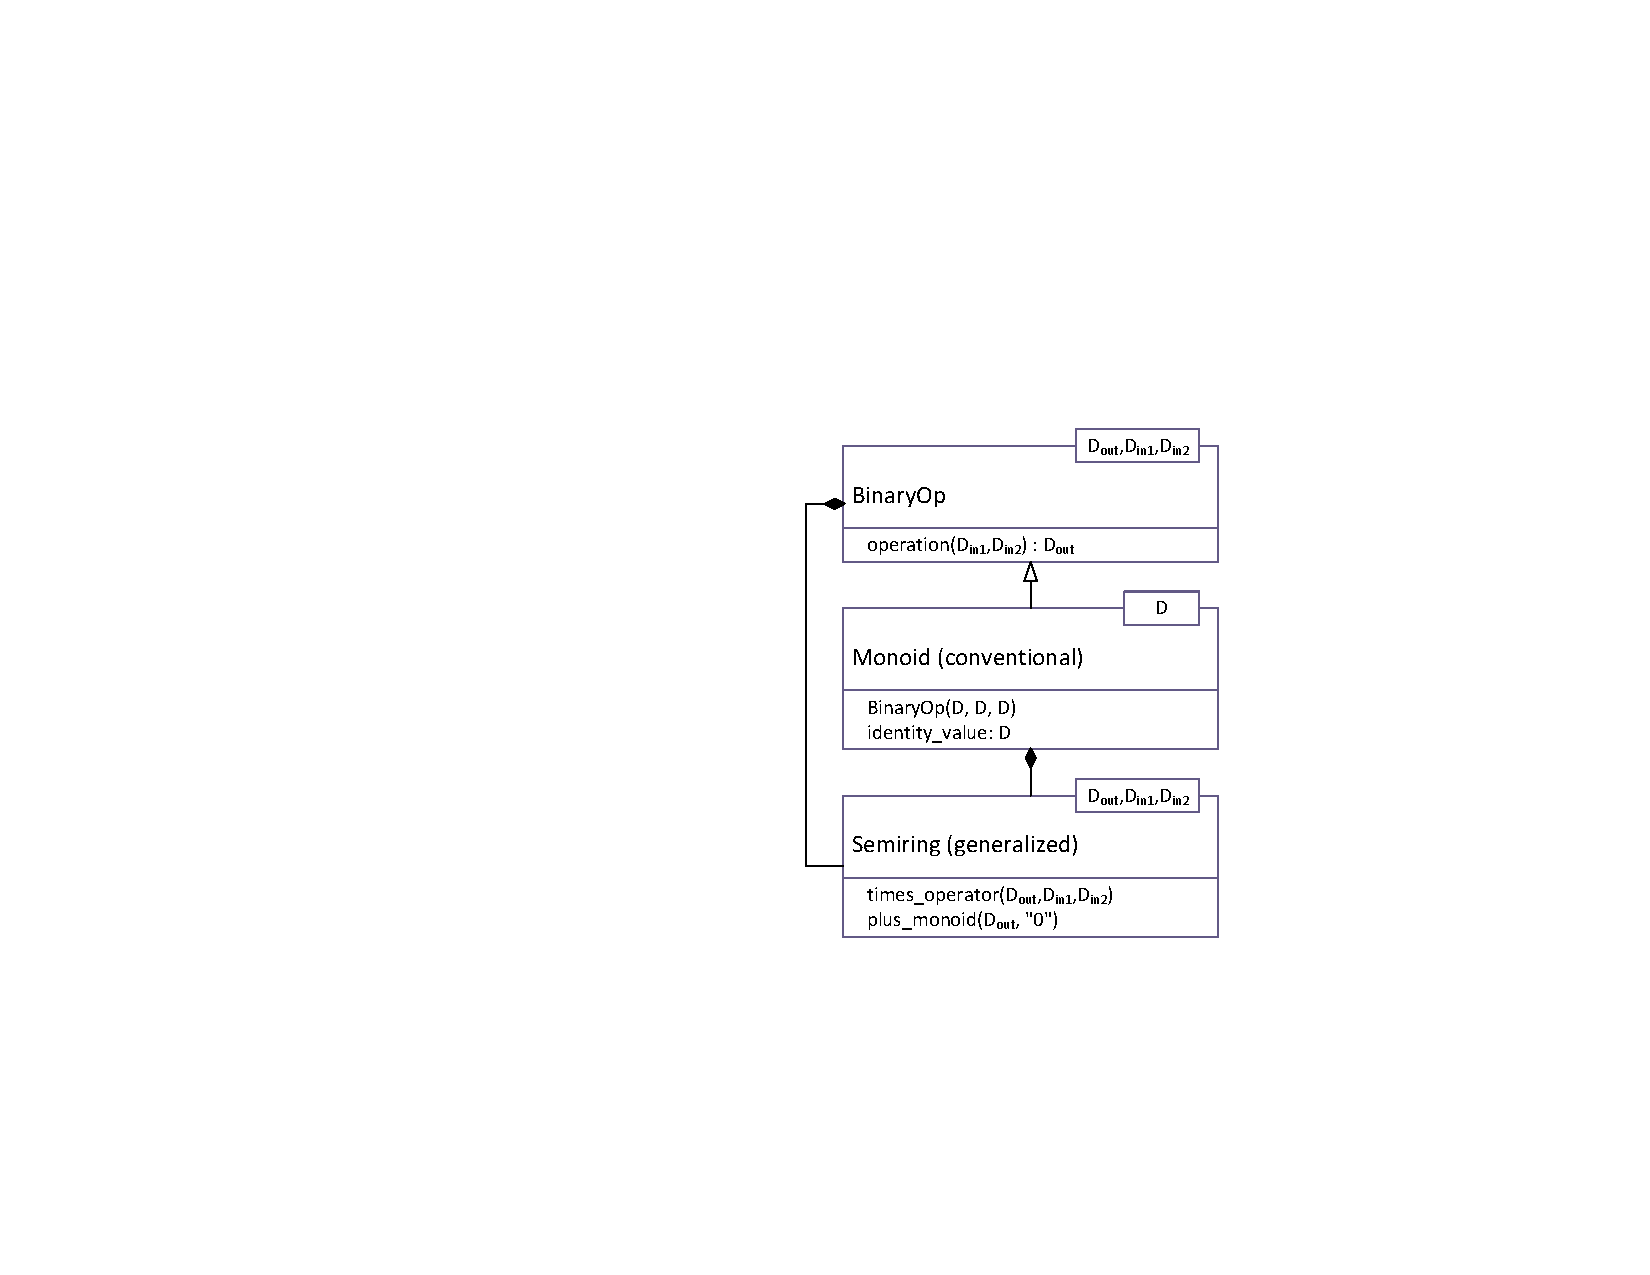
\includegraphics[width=1.0\linewidth,trim=3in 2in 0.5in 2in]{Algebra_Hierarchy_v2_1.pdf}
    \end{center}
    \caption{Hierarchy of algebraic object classes in GraphBLAS. GraphBLAS 
    semirings consist of a conventional monoid with one domain for the addition 
    function, and a binary operator with three domains for the multiplication function.}
    \label{Fig:AlgebraHierarchy}
    \hrule
\end{figure}

\section{Scalars \scott{NEW CONTENT}}
\label{Sec:Scalars}

A scalar $\scalar{s} = \langle D, \{ s_0 \} \rangle$ is defined by
a domain $D$, and a set of zero or one value $s_0$ where  $s_0 \in D$. 
We define $\mathbf{size}(\scalar{s}) = 1$ and
$\mathbf{L}(\scalar{s}) = \{ s_0 \}$. The set $\mathbf{L}(\scalar{s})$ is
called the \emph{content} of scalar $\scalar{s}$. We also define $\mathbf{D}(\scalar{s})
= D$. For a scalar $\scalar{s}$, $\scalar{s}(0)$ is a reference to $s_0$
if the scalar is not empty, and is undefined otherwise.

\section{Vectors}
\label{Sec:Vectors}

A vector $\vector{v} = \langle D, N, \{ (i,v_i) \} \rangle$ is defined by
a domain $D$, a size $N>0$, and a set of tuples $(i,v_i)$ where $0 \leq
i < N$ and $v_i \in D$. A particular value of $i$ can appear at
most once in $\vector{v}$. We define $\mathbf{size}(\vector{v}) = N$ and
$\mathbf{L}(\vector{v}) = \{ (i,v_i) \}$. The set $\mathbf{L}(\vector{v})$ is
called the \emph{content} of vector $\vector{v}$. We also define the set
$\vector{ind(\vector{v})} = \{ i : (i,v_i) \in \mathbf{L}(\vector{v}) \}$
(called the \emph{structure} of $\vector{v}$), and $\mathbf{D}(\vector{v})
= D$. For a vector $\vector{v}$, $\vector{v}(i)$ is a reference to $v_i$
if $(i,v_i) \in \mathbf{L}(\vector{v})$ and is undefined otherwise.

\section{Matrices}
\label{Sec:Matrices}

A matrix $\matrix{A} = \langle D, M, N, \{ (i,j,A_{ij}) \} \rangle$ is
defined by a domain $D$, its number of rows $M>0$, its number of columns
$N>0$, and a set of tuples $(i,j,A_{ij})$ where $0 \leq i < M$, $0 \leq
j < N$, and $A_{ij} \in D$. A particular pair of values $i,j$ can
appear at most once in $\matrix{A}$. We define $\mathbf{ncols}(\matrix{A})
= N$,  $\mathbf{nrows}(\matrix{A}) = M$, and $\mathbf{L}(\matrix{A}) =
\{ (i,j,A_{ij}) \}$.  The set $\mathbf{L}(\matrix{A})$ is called the
\emph{content} of matrix $\matrix{A}$.  We also define the sets
$\vector{indrow(\matrix{A})} = \{ i : \exists (i,j,A_{ij}) \in
\matrix{A} \}$ and $\vector{indcol(\matrix{A})} = \{ j : \exists
(i,j,A_{ij}) \in \matrix{A} \}$.  (These are the sets of nonempty
rows and columns of $\matrix{A}$, respectively.)  The \emph{structure}
of matrix $\matrix{A}$ is the set $\mathbf{ind}(\matrix{A}) = \{ (i,j) :
(i,j,A_{ij}) \in \mathbf{L}(\matrix{A}) \}$, and $\mathbf{D}(\matrix{A}) = D$.
For a matrix $\matrix{A}$, $\matrix{A}(i,j)$ is a reference to $A_{ij}$
if $(i,j,A_{ij}) \in \mathbf{L}(\matrix{A})$ and is undefined otherwise.

If $\matrix{A}$ is a matrix and $0 \leq j < N$, then $\matrix{A}(:,j)
= \langle D, M, \{(i,A_{ij}) : (i,j,A_{ij}) \in \mathbf{L}(\matrix{A})
\} \rangle$ is a vector called the $j$-th \emph{column}
of $\matrix{A}$. Correspondingly, if $\matrix{A}$ is a matrix and
$0 \leq i < M$, then $\matrix{A}(i,:) = \langle D, N, \{(j,A_{ij}) :
(i,j,A_{ij}) \in \mathbf{L}(\matrix{A}) \} \rangle$ is a vector called
the $i$-th \emph{row} of $\matrix{A}$.

Given a matrix $\matrix{A} = \langle D, M, N, \{ (i,j,A_{ij}) \} \rangle$,
its \emph{transpose} is another matrix $\matrix{A}^T = \langle D, N, M, \{
(j,i,A_{ij}) : (i,j,A_{ij}) \in \mathbf{L}(\matrix{A}) \} \rangle$.

\section{Masks}
\label{Sec:Masks}

The GraphBLAS C API defines an opaque object called a \emph{mask}.  The mask
is used to control how computed values are stored in the output from a method. 
The mask is an \emph{internal} opaque object; that is, it is never exposed as a variable
within an application. 

The mask is formed from objects input to the method that uses 
the mask.  For example, a GraphBLAS method may be called with a matrix as the mask
parameter.   The internal mask object is constructed from the input matrix in one
of two ways.  In the default case, an element of the mask is created for each 
tuple that exists in the matrix for which the value of the tuple cast to Boolean 
evaluates to {\tt true}.  Alternatively, the user can specify {\em structure}-only behavior where
an element of the mask is created for each tuple that exists in the matrix 
{\em regardless} of the value stored in the input matrix.
\scott{STRUCTURE\_ONLY changes.}

The internal mask object can be either a one- or a two-dimensional construct.  One- and
two-dimensional masks, described more formally below, are similar to
vectors and matrices, respectively, except that they have structure
(indices) but no values.  When needed, a value is implied for the elements of a 
mask with an implied value of {\tt true} for elements that exist 
and an implied value of {\tt false} for elements that do not exist (\ie,
the locations of the mask that do not have a stored value imply a value of {\tt false}).
Hence, even though a mask does not contain any values, it can be 
considered to imply values from a Boolean domain.

A one-dimensional mask $\vector{m} = \langle N, \{ i \} \rangle$ is
defined by its number of elements $N>0$, and a set $\mathbf{ind}(\vector{m})$
of indices $\{ i \}$ where $0 \leq i < N$.  A particular value of $i$ can
appear at most once in $\vector{m}$. We define $\mathbf{size}(\vector{m})
= N$. The set $\mathbf{ind}(\vector{m})$ is called the \emph{structure} of mask $\vector{m}$.

A two-dimensional mask $\matrix{M} = \langle M, N, \{ (i,j) \}
\rangle$ is defined by its number of rows $M>0$, its number of
columns $N>0$, and a set $\mathbf{ind}(\matrix{M})$ of tuples $(i,j)$
where $0 \leq i < M$, $0 \leq j < N$.   A particular pair of values
$i,j$ can appear at most once in $\matrix{M}$.  We define
$\mathbf{ncols}(\matrix{M}) = N$, and $\mathbf{nrows}(\matrix{M}) = M$.
We also define the sets $\vector{indrow(\matrix{M})} = \{ i : \exists
(i,j) \in \mathbf{ind}(\matrix{M}) \}$ and $\vector{indcol(\matrix{M})}
= \{ j : \exists (i,j) \in \mathbf{ind}(\matrix{M}) \}$.  These are
the sets of nonempty rows and columns of $\matrix{M}$, respectively.
The set $\mathbf{ind}(\matrix{M})$ is called the \emph{structure} of mask $\matrix{M}$.

One common operation on masks is the \emph{complement}.
For a one-dimensional mask $\vector{m}$ this is denoted as
$\neg\vector{m}$. For a two-dimensional masks, this is denoted as
$\neg\matrix{M}$.  The complement of a one-dimensional
mask $\vector{m}$ is defined as $\mathbf{ind}(\neg\vector{m}) = \{i : 0
\leq i < N, i \notin \mathbf{ind}(\vector{m}) \}$.  It is the set of all
possible indices that do not appear in $\vector{m}$.  The 
complement of a two-dimensional mask $\matrix{M}$ is defined as the set
$\mathbf{ind}(\neg\matrix{M}) = \{(i,j)$ : $0 \leq i < M$, $0 \leq j < N$,
$(i,j) \notin \mathbf{ind}(\matrix{M}) \}$.  It is the set of all possible
indices that do not appear in $\matrix{M}$.

\section{Descriptors}
\label{Sec:Descriptors}

Descriptors are used to modify the behavior of a GraphBLAS method.
When present in the signature of a method, they appear as the last
argument in the method.  Descriptors specify how the other input arguments
corresponding to GraphBLAS collections -- vectors, matrices, and masks
-- should be processed (modified) before the main operation of a method
is performed.

The descriptor is a lightweight object.  It is composed of (\emph{field},
\emph{value}) pairs where the \emph{field} selects one of the GraphBLAS objects
from the argument list of a method and the \emph{value} defines the
indicated modification associated with that object.  For example,
a descriptor may specify that a particular input matrix needs to be
transposed or that a mask needs to be complemented (defined
in Section~\ref{Sec:Masks}) before using it in the operation.

For the purpose of constructing descriptors, the arguments of a method
that can be modified are identified by specific field names. The output
parameter (typically the first parameter in a GraphBLAS method) is
indicated by the field name, {\sf GrB\_OUTP}.  The mask is indicated
by the {\sf GrB\_MASK} field name. The input parameters corresponding
to the input vectors and matrices are indicated by {\sf GrB\_INP0}
and {\sf GrB\_INP1} in the order they appear in the signature of the
GraphBLAS method.  The descriptor is an opaque object and hence we do not
define how objects of this type should be implemented.   When referring to
(\emph{field}, \emph{value}) pairs for a descriptor, however, we often use the informal
notation {\sf desc[GrB\_Desc\_Field].GrB\_Desc\_Value} without implying
that a descriptor is to be implemented as an array of structures (in fact,
field values can be used in conjunction with multiple values that are composable).
We summarize all types, field names, and values used with descriptors
in Table~\ref{Tab:DescTypeLiterals}.

\begin{table}
\hrule
\begin{center}
\caption{Descriptors are GraphBLAS objects passed as arguments to Graph\_BLAS 
operations to modify other GraphBLAS objects in the operation's argument list.
A descriptor, {\sf desc}, has one or more (\emph{field}, \emph{value}) pairs indicated 
as  {\sf desc[GrB\_Desc\_Field].GrB\_Desc\_Value}. In this table, we define all types and literals used
with descriptors.}
\label{Tab:DescTypeLiterals}

\vspace{1\baselineskip}
(a) Types used with GraphBLAS descriptors.
\vspace{1\baselineskip}

\begin{tabular}{l|l}
Type			& Description \\ \hline
{\sf GrB\_Descriptor}     &  Type of a GraphBLAS descriptor object. \\
{\sf GrB\_Desc\_Field}              &  Type of a descriptor field. \\
{\sf GrB\_Desc\_Value}             &  Type of a descriptor field's value. \\
\end{tabular}

\vspace{1\baselineskip}
(b) Descriptor field names of type {\sf GrB\_Desc\_Field}.
\vspace{1\baselineskip}

\begin{tabular}{l|l}
Field name          & Description \\ \hline
{\sf GrB\_OUTP} &  Field name for the output GraphBLAS object. \\
{\sf GrB\_INP0}   &  Field name for the first input GraphBLAS object. \\
{\sf GrB\_INP1}   &  Field name for the second input  GraphBLAS object. \\
{\sf GrB\_MASK} &  Field name for the mask GraphBLAS object. \\\
\end{tabular}

\vspace{1\baselineskip}
(c) Descriptor field values of type {\sf GrB\_Desc\_Value}.
\scott{STRUCTURE\_ONLY changes.}
\vspace{1\baselineskip}

\begin{tabular}{l|l}
Field Value          & Description \\ \hline
{\sf GrB\_STRUCTURE} &  The write mask is constructed from the structure (pattern of stored \\
                     &  values) of the associated object. The stored values are not examined.\\
{\sf GrB\_COMP}      &  Use the complement of the associated object. When combined \\ 
                     &  with {\sf GrB\_STRUCTURE}, the complement of the structure of the associated \\
                     &  object is used without evaluating the values stored.\\
{\sf GrB\_SCMP}      &  Use the complement of the associated object. When combined \\ 
                     &  with {\sf GrB\_STRUCTURE}, the complement of the structure of the associated \\
             &  object is used without evaluating the values stored. {\color{red} This field value} \\
		     &  {\color{red} is currently deprecated in favor of {\sf GrB\_COMP} above, and may be} \\
		     &  {\color{red} removed in future versions of this API.} \\
{\sf GrB\_TRAN}      &  Use the transpose of the associated object.\\
{\sf GrB\_REPLACE}   &  Clear the output object before assigning computed values.\\
\end{tabular}
\end{center}
\hrule
\end{table}

In the definitions of the GraphBLAS methods, we often refer to the
\emph{default behavior} of a method with respect to the action of a
descriptor.   If a descriptor is not provided or if the value associated
with a particular field in a descriptor is not set, the default behavior
of a GraphBLAS method is defined as follows:
\begin{itemize}
\item Input matrices are not transposed.
\item The mask is used, as is, without complementing, and stored values are examined to 
determine whether they evaluate to {\tt true} or {\tt false}.\scott{STRUCTURE\_ONLY changes.}

\item Values of the output object that are not directly modified by the operation are preserved.
\end{itemize}

GraphBLAS specifies a set of pre-defined descriptors. Their identifiers
and the corresponding set of (field,value) pairs for that
identfier are shown in Table~\ref{Tab:DefaultDescriptors}.

\newcommand{\grboutp}{{\sf GrB\_OUTP}}
\newcommand{\grbmask}{{\sf GrB\_MASK}}
\newcommand{\grbinp}[1]{{\sf GrB\_INP#1}}
\newcommand{\grbreplace}{{\sf GrB\_REPLACE}}
\newcommand{\grbstructure}{{\sf GrB\_STRUCTURE}}
\newcommand{\grbscmp}{{\sf GrB\_COMP}}

\newcommand{\grbrepl}{{\sf GrB\_REPLACE}}
\newcommand{\grbstrc}{{\sf GrB\_STRUCTURE}}
\newcommand{\grbcomp}{{\sf GrB\_COMP}}
\newcommand{\grbtran}{{\sf GrB\_TRAN}}

\begin{table}[htbp]
    \hrule
    \begin{center}
	\caption{Pre-defined GraphBLAS descriptors. The list includes
	all possible descriptors, according to the current standard.  Columns list the
    possible fields and entries list the value(s) associated with those fields for
    a given descriptor.}
	\label{Tab:DefaultDescriptors}
~\\
	\begin{small}

        \begin{tabular}{l|llll} 
        Identifier          & {\sf GrB\_OUTP} & {\sf GrB\_MASK} & {\sf GrB\_INP0} & {\sf GrB\_INP1}  \\ \hline
        {\sf GrB\_NULL}     &    --    &    --    &    --    &    --    \\
        {\sf GrB\_DESC\_T1}       &    --    &    --    &    --    & \grbtran \\
        {\sf GrB\_DESC\_T0}       &    --    &    --    & \grbtran &    --    \\
        {\sf GrB\_DESC\_T0T1}     &    --    &    --    & \grbtran & \grbtran \\
        {\sf GrB\_DESC\_C}        &    --    & \grbcomp &    --    &    --    \\
        {\sf GrB\_DESC\_S}        &    --    & \grbstrc &    --    &    --    \\
        {\sf GrB\_DESC\_CT1}      &    --    & \grbcomp &    --    & \grbtran \\
        {\sf GrB\_DESC\_ST1}      &    --    & \grbstrc &    --    & \grbtran \\
        {\sf GrB\_DESC\_CT0}      &    --    & \grbcomp & \grbtran &    --    \\
        {\sf GrB\_DESC\_ST0}      &    --    & \grbstrc & \grbtran &    --    \\
        {\sf GrB\_DESC\_CT0T1}    &    --    & \grbcomp & \grbtran & \grbtran \\
        {\sf GrB\_DESC\_ST0T1}    &    --    & \grbstrc & \grbtran & \grbtran \\
        {\sf GrB\_DESC\_SC}       &    --    & \grbstrc, \grbcomp &    --    &    --    \\
        {\sf GrB\_DESC\_SCT1}     &    --    & \grbstrc, \grbcomp &    --    & \grbtran \\
        {\sf GrB\_DESC\_SCT0}     &    --    & \grbstrc, \grbcomp & \grbtran &    --    \\
        {\sf GrB\_DESC\_SCT0T1}   &    --    & \grbstrc, \grbcomp & \grbtran & \grbtran \\
        {\sf GrB\_DESC\_R}        & \grbrepl &    --    &    --    &    --    \\
        {\sf GrB\_DESC\_RT1}      & \grbrepl &    --    &    --    & \grbtran \\
        {\sf GrB\_DESC\_RT0}      & \grbrepl &    --    & \grbtran &    --    \\
        {\sf GrB\_DESC\_RT0T1}    & \grbrepl &    --    & \grbtran & \grbtran \\
        {\sf GrB\_DESC\_RC}       & \grbrepl & \grbcomp &    --    &    --    \\
        {\sf GrB\_DESC\_RS}       & \grbrepl & \grbstrc &    --    &    --    \\
        {\sf GrB\_DESC\_RCT1}     & \grbrepl & \grbcomp &    --    & \grbtran \\
        {\sf GrB\_DESC\_RST1}     & \grbrepl & \grbstrc &    --    & \grbtran \\
        {\sf GrB\_DESC\_RCT0}     & \grbrepl & \grbcomp & \grbtran &    --    \\
        {\sf GrB\_DESC\_RST0}     & \grbrepl & \grbstrc & \grbtran &    --    \\
        {\sf GrB\_DESC\_RCT0T1}   & \grbrepl & \grbcomp & \grbtran & \grbtran \\
        {\sf GrB\_DESC\_RST0T1}   & \grbrepl & \grbstrc & \grbtran & \grbtran \\
        {\sf GrB\_DESC\_RSC}      & \grbrepl & \grbstrc, \grbcomp &    --    &    --    \\
        {\sf GrB\_DESC\_RSCT1}    & \grbrepl & \grbstrc, \grbcomp &    --    & \grbtran \\
        {\sf GrB\_DESC\_RSCT0}    & \grbrepl & \grbstrc, \grbcomp & \grbtran &    --    \\
        {\sf GrB\_DESC\_RSCT0T1}  & \grbrepl & \grbstrc, \grbcomp & \grbtran & \grbtran \\
        \end{tabular}
	\end{small}

    \end{center}
    \hrule
\end{table}



\section{Methods}
\label{Sec:Methods}

\subsection{Algebra Methods}
\label{Sec:AlgebraMethods}

%-----------------------------------------------------------------------------

\subsubsection{{\sf Type\_new}: Create a new GraphBLAS (user-defined) type}
\label{Sec:TypeNew}

Creates a new user-defined GraphBLAS type. This type can then be used to create new
operators, monoids, semirings, vectors and matrices.

\paragraph{\syntax}

\begin{verbatim}
        GrB_Info GrB_Type_new(GrB_Type  *utype,
                              size_t     sizeof(ctype));
\end{verbatim}

\paragraph{Parameters}

\begin{itemize}[leftmargin=1.1in]
    \item[{\sf utype}] ({\sf INOUT}) On successful return, contains a handle 
                                     to the newly created user-defined GraphBLAS 
                                     type object.
	\item[{\sf ctype}] ({\sf IN})    A C type that defines the new GraphBLAS 
                                     user-defined type.
\end{itemize}

\paragraph{Return Values}

\begin{itemize}[leftmargin=2.1in]
\item[{\sf GrB\_SUCCESS}]           operation completed successfully.
\item[{\sf GrB\_PANIC}]             unknown internal error.
\item[{\sf GrB\_OUT\_OF\_MEMORY}]          not enough memory available for operation.
\item[{\sf GrB\_NULL\_POINTER}]    {\sf utype} pointer is {\sf NULL}.
\end{itemize}

\paragraph{Description}

Given a C type {\sf ctype}, the {\sf Type\_new} method returns in {\sf utype} a handle to
a new GraphBLAS type that is equivalent to the C type.  Variables of this {\sf ctype} 
must be a struct, union, or fixed-size array. In particular, given two variables, 
{\tt src} and {\tt dst}, of type {\sf ctype}, the following operation must be a 
valid way to copy the contents of {\tt src} to {\tt dst}:

\begin{center}
{\tt memcpy(\&dst, \&src, sizeof({\sf ctype}))}
\end{center}

A new, user-defined type {\sf utype} should be destroyed with a call to 
{\sf GrB\_free(utype)} when no longer needed.

It is not an error to call this method more than once on the same variable;  
however, the handle to the previously created object will be overwritten. 

%-----------------------------------------------------------------------------
\subsubsection{{\sf UnaryOp\_new}: Create a new GraphBLAS unary operator}

Initializes a new GraphBLAS unary operator with a specified user-defined 
function and its types (domains).

\paragraph{\syntax}

\begin{verbatim}
        GrB_Info GrB_UnaryOp_new(GrB_UnaryOp *unary_op,
                                 void       (*unary_func)(void*, const void*),
                                 GrB_Type     d_out,
                                 GrB_Type     d_in);
\end{verbatim}

\paragraph{Parameters}

\begin{itemize}[leftmargin=1.1in]
    \item[{\sf unary\_op}] ({\sf INOUT}) On successful return, contains a
                           handle to the newly created GraphBLAS unary operator object.
    \item[{\sf unary\_func}] ({\sf IN})  a pointer to a user-defined function that takes 
                           one input parameter of {\sf d\_in}'s type
			   and returns a value of {\sf d\_out}'s type, both passed as {\sf void} pointers.
                           Specifically the signature of the function is expected to 
                           be of the form:
          \begin{verbatim}
          void func(void *out, const void *in);
          \end{verbatim}
    \item[{\sf d\_out}] ({\sf IN})  The {\sf GrB\_Type} of the return value of the unary 
                           operator being created.  Should be one of the predefined 
                           GraphBLAS types in Table~\ref{Tab:PredefinedTypes}, or a 
                           user-defined GraphBLAS type.
    \item[{\sf d\_in}] ({\sf IN})  The {\sf GrB\_Type} of the input 
                           argument of the unary operator being created.  Should be 
                           one of the predefined GraphBLAS types in 
                           Table~\ref{Tab:PredefinedTypes}, or a user-defined GraphBLAS type.
\end{itemize}

\paragraph{Return Values}

\begin{itemize}[leftmargin=2.1in]
\item[{\sf GrB\_SUCCESS}]           operation completed successfully.
\item[{\sf GrB\_PANIC}]             unknown internal error.
\item[{\sf GrB\_OUT\_OF\_MEMORY}]          not enough memory available for operation.
\item[{\sf GrB\_UNINITIALIZED\_OBJECT}]          any {\sf GrB\_Type} parameter (for
                                    user-defined types) has not been
                                    initialized by a call to {\sf GrB\_Type\_new}.
\item[{\sf GrB\_NULL\_POINTER}]    {\sf unary\_op} or {\sf unary\_func}
                                    pointers are {\sf NULL}.

\jose{Domain mismatch not possible.}
%\item[{\sf GrB\_DOMAIN\_MISMATCH}]  the types in the function pointer signature
%                                    are not compatible with the {\sf GrB\_Type}
%                                    parameters specified when user-defined types
%                                    are specified.
\end{itemize}

\paragraph{Description}

\newenvironment{code}{\tt}{}

The {\sf UnaryOp\_new} method creates a new GraphBLAS unary operator
\begin{quote}
$f_u = \langle \mathbf{D}({\sf d\_out}), \mathbf{D}({\sf d\_in}), {\sf unary\_func} \rangle$
\end{quote}
and returns a handle to it in {\sf unary\_op}.

The implementation of {\sf unary\_func} must be such that it works
even if the {\sf d\_out} and {\sf d\_in} arguments are aliased.
In other words, for all invocations of the function:
\begin{quote}
\begin{verbatim}
unary_func(out,in);
\end{verbatim}
\end{quote}
the value of {\sf out} must be the same as if the following code
was executed:

\begin{quote}
\begin{code}
    $\mathbf{D}({\sf d\_in})$ tmp = malloc(sizeof($\mathbf{D}({\sf d\_in}$))); \\
    memcpy(tmp,in,sizeof($\mathbf{D}({\sf d\_in}$))); \\
    unary\_func(out,tmp); \\
    free(tmp);
\end{code}
\end{quote}

It is not an error to call this method more than once on the same variable;  
however, the handle to the previously created object will be overwritten. 

%-----------------------------------------------------------------------------

\subsubsection{{\sf BinaryOp\_new}: Create a new GraphBLAS binary operator}

Initializes a new GraphBLAS binary operator with a specified user-defined 
function and its types (domains).

\paragraph{\syntax}

\begin{verbatim}
        GrB_Info GrB_BinaryOp_new(GrB_BinaryOp *binary_op,
                                  void        (*binary_func)(void*,
                                                             const void*,
                                                             const void*),
                                  GrB_Type      d_out,
                                  GrB_Type      d_in1,
                                  GrB_Type      d_in2);
\end{verbatim}

\paragraph{Parameters}

\begin{itemize}[leftmargin=1.1in]
    \item[{\sf binary\_op}] ({\sf INOUT}) On successful return, contains a 
          handle to the newly created GraphBLAS binary operator object.
    \item[{\sf binary\_func}] ({\sf IN}) A pointer to a user-defined function that 
          takes two input parameters of types {\sf d\_in1} and {\sf d\_in2} and returns a value of
		type {\sf d\_out}, all passed as {\sf void} pointers.
          Specifically the signature of the function is expected to 
          be of the form:
      \begin{verbatim}
      void func(void *out, const void *in1, const void *in2);
      \end{verbatim}
    \item[{\sf d\_out}]  ({\sf IN}) The {\sf GrB\_Type} of the return
          value of the binary operator being created. Should be one of the
          predefined GraphBLAS types in Table~\ref{Tab:PredefinedTypes}, or a 
          user-defined GraphBLAS type.
    \item[{\sf d\_in1}]  ({\sf IN}) The {\sf GrB\_Type} of the left hand 
          argument of the binary operator being created. Should be one of the
          predefined GraphBLAS types in Table~\ref{Tab:PredefinedTypes}, or a
          user-defined GraphBLAS type.
    \item[{\sf d\_in2}]  ({\sf IN}) The {\sf GrB\_Type} of the right hand 
          argument of the binary operator being created. Should be one of the
          predefined GraphBLAS types in Table~\ref{Tab:PredefinedTypes}, or a 
          user-defined GraphBLAS type.
\end{itemize}

\paragraph{Return Values}

\begin{itemize}[leftmargin=2.1in]
\item[{\sf GrB\_SUCCESS}]           operation completed successfully.
\item[{\sf GrB\_PANIC}]             unknown internal error.
\item[{\sf GrB\_OUT\_OF\_MEMORY}]          not enough memory available for operation.
\item[{\sf GrB\_UNINITIALIZED\_OBJECT}]          the {\sf GrB\_Type} (for user-defined types)
                                    has not been initialized by a call to {\sf GrB\_Type\_new}.
\item[{\sf GrB\_NULL\_POINTER}]    {\sf binary\_op} or {\sf binary\_func} pointer is {\sf NULL}.

\jose{Domain mistmatch not possible.}
%\item[{\sf GrB\_DOMAIN\_MISMATCH}]  the types in the function pointer signature are not   
%                                    compatible with the {\sf GrB\_Type} parameters specified.
\end{itemize}

\paragraph{Description}

The {\sf BinaryOp\_new} methods creates a new GraphBLAS binary operator
\begin{quote}
$f_b = \langle \mathbf{D}({\sf d\_out}), \mathbf{D}({\sf d\_in1}), \mathbf{D}({\sf d\_in2}), {\sf binary\_func} \rangle$
\end{quote}
and returns a handle to it in {\sf binary\_op}.

The implementation of {\sf binary\_func} must be such that it works
even if any of the {\sf d\_out}, {\sf d\_in1}, and {\sf d\_in2} arguments are aliased to each other.
In other words, for all invocations of the function:
\begin{quote}
\begin{verbatim}
binary_func(out,in1,in2);
\end{verbatim}
\end{quote}
the value of {\sf out} must be the same as if the following code
was executed:

\begin{quote}
\begin{code}
    $\mathbf{D}({\sf d\_in1})$ tmp1 = malloc(sizeof($\mathbf{D}({\sf d\_in1}$))); \\
    $\mathbf{D}({\sf d\_in2})$ tmp2 = malloc(sizeof($\mathbf{D}({\sf d\_in2}$))); \\
    memcpy(tmp1,in1,sizeof($\mathbf{D}({\sf d\_in1}$))); \\
    memcpy(tmp2,in2,sizeof($\mathbf{D}({\sf d\_in2}$))); \\
    binary\_func(out,tmp1,tmp2); \\
    free(tmp2); \\
    free(tmp1);
\end{code}
\end{quote}

It is not an error to call this method more than once on the same variable;  
however, the handle to the previously created object will be overwritten. 

%-----------------------------------------------------------------------------

\subsubsection{{\sf Monoid\_new}: Create new GraphBLAS monoid}

Creates a new monoid with specified binary operator and identity value.

\paragraph{\syntax}

\begin{verbatim}
        GrB_Info GrB_Monoid_new(GrB_Monoid    *monoid,
                                GrB_BinaryOp   binary_op,
                                <type>         identity);
\end{verbatim}

\paragraph{Parameters}

\begin{itemize}[leftmargin=1.1in]
    \item[{\sf monoid}] ({\sf INOUT}) On successful return, contains a
                         handle to the newly created GraphBLAS monoid object.
    \item[{\sf binary\_op}] ({\sf IN}) An existing GraphBLAS associative binary 
                         operator whose input and output types are the same.
    \item[{\sf identity}]  ({\sf IN}) The value of the identity element of the 
                         monoid. Must be the same type as the type used by the
                         {\sf binary\_op} operator.
\end{itemize}

\paragraph{Return Values}

\begin{itemize}[leftmargin=2.1in]
\item[{\sf GrB\_SUCCESS}]           operation completed successfully.
\item[{\sf GrB\_PANIC}]             unknown internal error.
\item[{\sf GrB\_OUT\_OF\_MEMORY}]   not enough memory available for operation.
\item[{\sf GrB\_UNINITIALIZED\_OBJECT}]  the {\sf GrB\_BinaryOp} has not been
                                    initialized by a call to {\sf GrB\_BinaryOp\_new}.
\item[{\sf GrB\_NULL\_POINTER}]     {\sf monoid} pointer is {\sf NULL}.
\item[{\sf GrB\_DOMAIN\_MISMATCH}]  all three argument types of the binary operator and
                                    the type of the identity value are not the same.
\end{itemize}

\paragraph{Description}

The {\sf Monoid\_new} method creates a new monoid $M = \langle \mathbf{D}({\sf binary\_op}), {\sf binary\_op}, 
{\sf identity} \rangle$ and returns a handle to it in {\sf monoid}.

If {\sf binary\_op} is not associative, the results of GraphBLAS operations that
require associativity of this monoid will be undefined.

It is not an error to call this method more than once on the same variable;  
however, the handle to the previously created object will be overwritten. 

%-----------------------------------------------------------------------------
\subsubsection{{\sf Semiring\_new}: Create new GraphBLAS semiring}

Creates a new semiring with specified domain, operators, and elements.

\paragraph{\syntax}

\begin{verbatim}
        GrB_Info GrB_Semiring_new(GrB_Semiring  *semiring,
                                  GrB_Monoid     add_op,
                                  GrB_BinaryOp   mul_op);
\end{verbatim}

\paragraph{Parameters}

\begin{itemize}[leftmargin=1.1in]
    \item[{\sf semiring}] ({\sf INOUT}) On successful return, contains a 
    handle to the newly created GraphBLAS semiring.
    \item[{\sf add\_op}]  ({\sf IN}) An existing GraphBLAS commutative monoid that 
    specifies the addition operator and its identity.
    \item[{\sf mul\_op}]  ({\sf IN}) An existing GraphBLAS binary operator that 
    specifies the semiring's multiplication operator. In addition, {\sf mul\_op}'s
    output domain, $\bDout({\sf mul\_op})$, must be the same as the {\sf add\_op}'s
    domain $\mathbf{D}(\mbox{\sf add\_op})$.
\end{itemize}


\paragraph{Return Values}

\begin{itemize}[leftmargin=2.1in]
\item[{\sf GrB\_SUCCESS}]           operation completed successfully.
\item[{\sf GrB\_PANIC}]             unknown internal error.
\item[{\sf GrB\_OUT\_OF\_MEMORY}]   not enough memory available for this method to complete.
\item[{\sf GrB\_UNINITIALIZED\_OBJECT}]   the {\sf add\_op} object has not been
                                    initialized with a call to {\sf GrB\_Monoid\_new}
                                    or the {\sf mul\_op} object has not been
                                    not been initialized by a call to 
                                    {\sf GrB\_BinaryOp\_new}.
\item[{\sf GrB\_NULL\_POINTER}]    {\sf semiring} pointer is {\sf NULL}.
\item[{\sf GrB\_DOMAIN\_MISMATCH}]  the output domain of {\sf mul\_op} does not
                                    match the domain of the {\sf add\_op} monoid.
\end{itemize}

\paragraph{Description}

The {\sf Semiring\_new} method creates a new semiring:
\begin{quote}
$S = \langle \bDout({\sf mul\_op}), 
\bDin1({\sf mul\_op}), \bDin2({\sf mul\_op}), {\sf add\_op}, 
{\sf mul\_op}, \mathbf{0}({\sf add\_op})\rangle$
\end{quote}
and returns a handle to it in 
{\sf semiring}.  Note that $\bDout({\sf mul\_op})$ must be the same as 
$\mathbf{D}({\sf add\_op})$.

If {\sf add\_op} is not commutative, then GraphBLAS operations using this semiring
will be undefined.

It is not an error to call this method more than once on the same variable;  
however, the handle to the previously created object will be overwritten. 

%-----------------------------------------------------------------------------

\subsubsection{{\sf IndexUnaryOp\_new}: Create a new GraphBLAS index unary operator \scott{NEW CONTENT}}

Initializes a new GraphBLAS index unary operator with a specified user-defined 
function and its types (domains).

\paragraph{\syntax}

\begin{verbatim}
    GrB_Info GrB_IndexUnaryOp_new(GrB_IndexUnaryOp   *index_unary_op,
                                  void (*index_unary_func)(void*,
                                                           const void*,
                                                           GrB_Index*,
                                                           GrB_Index,
                                                           const void*),
                                  GrB_Type            d_out,
                                  GrB_Type            d_in1,
                                  GrB_Type            d_in2);
\end{verbatim}

\paragraph{Parameters}

\begin{itemize}[leftmargin=1.2in]
    \item[{\sf index\_unary\_op}] ({\sf INOUT}) On successful return, contains a 
          handle to the newly created GraphBLAS index unary operator object.
    \item[{\sf index\_unary\_func}] ({\sf IN}) A pointer to a user-defined 
          function that takes input parameters of types {\sf d\_in1}, 
          {\sf GrB\_Index} pointer, {\sf GrB\_Index} and {\sf d\_in2}
          and returns a value of type {\sf d\_out}.  Except for the {\sf GrB\_Index}
          parameters, all are passed as {\sf void} pointers.
          Specifically the signature of the function is expected to 
          be of the form:
      \begin{verbatim}
      void func(void *out,
                const void *in1, GrB_index* indices, GrB_Index n, 
                const void *in2);
      \end{verbatim}
    \item[{\sf d\_out}]  ({\sf IN}) The {\sf GrB\_Type} of the return
          value of the index unary operator being created. Should be one of the
          predefined GraphBLAS types in Table~\ref{Tab:PredefinedTypes}, or a 
          user-defined GraphBLAS type.
    \item[{\sf d\_in1}]  ({\sf IN}) The {\sf GrB\_Type} of the first input 
          argument of the index unary operator being created and corresponds to
          the stored values of the {\sf GrB\_Vector} or {\sf GrB\_Matrix} being
          operated on. Should be one of the predefined GraphBLAS types in
          Table~\ref{Tab:PredefinedTypes}, or a user-defined GraphBLAS type.
    \item[{\sf d\_in2}]  ({\sf IN}) The {\sf GrB\_Type} of the last input
          argument of the index unary operator being created and corresponds to
          a scalar provided by the GraphBLAS operation that uses this operator.
          Should be one of the predefined GraphBLAS types in 
          Table~\ref{Tab:PredefinedTypes}, or a user-defined GraphBLAS type.
\end{itemize}

\paragraph{Return Values}

\begin{itemize}[leftmargin=2.1in]
\item[{\sf GrB\_SUCCESS}]           operation completed successfully.
\item[{\sf GrB\_PANIC}]             unknown internal error.
\item[{\sf GrB\_OUT\_OF\_MEMORY}]          not enough memory available for operation.
\item[{\sf GrB\_UNINITIALIZED\_OBJECT}]          the {\sf GrB\_Type} (for user-defined types)
                                    has not been initialized by a call to {\sf GrB\_Type\_new}.
\item[{\sf GrB\_NULL\_POINTER}]    {\sf index\_unary\_op} or {\sf index\_unary\_func} pointer is {\sf NULL}.

\jose{Domain mistmatch not possible.}
%\item[{\sf GrB\_DOMAIN\_MISMATCH}]  the types in the function pointer signature are not   
%                                    compatible with the {\sf GrB\_Type} parameters specified.
\end{itemize}

\paragraph{Description}

The {\sf IndexUnaryOp\_new} methods creates a new GraphBLAS index unary operator
\begin{quote}
$f_{iu} = \langle \mathbf{D}({\sf d\_out}), \mathbf{D}({\sf d\_in1}), \mathbf{D}({\sf GrB\_Index}^n), \mathbf{D}({\sf GrB\_Index}), \mathbf{D}({\sf d\_in2}), {\sf index\_unary\_func} \rangle$
\end{quote}
and returns a handle to it in {\sf index\_unary\_op}.

The implementation of {\sf index\_unary\_func} must be such that it works
even if any of the {\sf d\_out}, {\sf d\_in1}, and {\sf d\_in2} arguments are aliased to each other.
In other words, for all invocations of the function:
\begin{quote}
\begin{verbatim}
index_unary_func(out,in1,&indices,n,in2);
\end{verbatim}
\end{quote}
the value of {\sf out} must be the same as if the following code
was executed (shown here for matrices):

\begin{quote}
\begin{code}
    \#define DIM 2;\\
    GrB\_Index indices[DIM];\\
    indices[0] = <row index>;\\
    indices[1] = <col index>;\\
    $\mathbf{D}({\sf d\_in1})$ tmp1 = malloc(sizeof($\mathbf{D}({\sf d\_in1}$))); \\
    $\mathbf{D}({\sf d\_in2})$ tmp2 = malloc(sizeof($\mathbf{D}({\sf d\_in2}$))); \\
    memcpy(tmp1,in1,sizeof($\mathbf{D}({\sf d\_in1}$))); \\
    memcpy(tmp2,in2,sizeof($\mathbf{D}({\sf d\_in2}$))); \\
    index\_unary\_func(out,tmp1,indices,DIM,tmp2); \\
    free(tmp2); \\
    free(tmp1);
\end{code}
\end{quote}

It is not an error to call this method more than once on the same variable;  
however, the handle to the previously created object will be overwritten. 

\subsection{Vector methods}

%-----------------------------------------------------------------------------
\subsubsection{{\sf Vector\_new}: Construct new vector}

Creates a new vector with specified domain and size.

\paragraph{\syntax}

\begin{verbatim}
        GrB_Info GrB_Vector_new(GrB_Vector *v,
                                GrB_Type    d,
                                GrB_Index   nsize);
\end{verbatim}

\paragraph{Parameters}

\begin{itemize}[leftmargin=1.1in]
    \item[{\sf v}] ({\sf INOUT}) On successful return, contains a handle
                                 to the newly created GraphBLAS vector.
    \item[{\sf d}] ({\sf IN})    The type corresponding to the domain of the 
                                 vector being created.  Can be one of the 
                                 predefined GraphBLAS types in 
                                 Table~\ref{Tab:PredefinedTypes}, or an existing 
                                 user-defined GraphBLAS type.
    \item[{\sf nsize}] ({\sf IN}) The size of the vector being created.
\end{itemize}

\paragraph{Return Values}

\begin{itemize}[leftmargin=2.1in]
    \item[{\sf GrB\_SUCCESS}]         In blocking mode, the operation completed
    successfully. In non-blocking mode, this indicates that the API checks 
    for the input arguments passed successfully. Either way, output vector 
    {\sf v} is ready to be used in the next method of the sequence.

    \item[{\sf GrB\_PANIC}]           Unknown internal error.
    
    \item[{\sf GrB\_INVALID\_OBJECT}] This is returned in any execution mode 
    whenever one of the opaque GraphBLAS objects (input or output) is in an invalid 
    state caused by a previous execution error.  Call {\sf GrB\_error()} to access 
    any error messages generated by the implementation.

    \item[{\sf GrB\_OUT\_OF\_MEMORY}] Not enough memory available for operation.
    
    \item[{\sf GrB\_UNINITIALIZED\_OBJECT}]  The {\sf GrB\_Type} object has not 
    been initialized by a call to {\sf GrB\_Type\_new} (needed for user-defined types).
    
    \item[{\sf GrB\_NULL\_POINTER}]  The {\sf v} pointer is {\sf NULL}.
    
    \item[{\sf GrB\_INVALID\_VALUE}] {\sf nsize} is zero or outside the range of the type {\sf GrB\_Index}.
\end{itemize}

\paragraph{Description}

Creates a new vector $\vector{v}$ of domain $\mathbf{D}({\sf d})$, size {\sf nsize}, 
and empty $\mathbf{L}(\vector{v})$. The method returns a handle to the new vector in {\sf v}.

It is not an error to call this method more than once on the same variable;  
however, the handle to the previously created object will be overwritten. 

%-----------------------------------------------------------------------------
\subsubsection{{\sf Vector\_dup}: Construct a copy of a GraphBLAS vector}

Creates a new vector with the same domain, size, and contents as another vector.

\paragraph{\syntax}

\begin{verbatim}
        GrB_Info GrB_Vector_dup(GrB_Vector       *w,
                                const GrB_Vector  u);
\end{verbatim}

\paragraph{Parameters}

\begin{itemize}[leftmargin=1.1in]
    \item[{\sf w}]  ({\sf INOUT}) On successful return, contains a handle
                                  to the newly created GraphBLAS vector.
    \item[{\sf u}]  ({\sf IN})    The GraphBLAS vector to be duplicated.
\end{itemize}

\paragraph{Return Values}

\begin{itemize}[leftmargin=2.1in]
    \item[{\sf GrB\_SUCCESS}]         In blocking mode, the operation completed
    successfully. In non-blocking mode, this indicates that the API checks 
    for the input arguments passed successfully. Either way, output vector 
    {\sf w} is ready to be used in the next method of the sequence.

    \item[{\sf GrB\_PANIC}]           Unknown internal error.
    
    \item[{\sf GrB\_INVALID\_OBJECT}] This is returned in any execution mode 
    whenever one of the opaque GraphBLAS objects (input or output) is in an invalid 
    state caused by a previous execution error.  Call {\sf GrB\_error()} to access 
    any error messages generated by the implementation.

    \item[{\sf GrB\_OUT\_OF\_MEMORY}] Not enough memory available for operation.
    
    \item[{\sf GrB\_UNINITIALIZED\_OBJECT}]  The GraphBLAS vector, {\sf u}, has 
    not been initialized by a call to {\sf Vector\_new} or {\sf Vector\_dup}.
    
    \item[{\sf GrB\_NULL\_POINTER}]  The {\sf w} pointer is {\sf NULL}.
\end{itemize}

\paragraph{Description}

Creates a new vector $\vector{w}$ of domain $\mathbf{D}({\sf u})$, size 
$\mathbf{size}({\sf u})$, and contents $\mathbf{L}({\sf u})$. The method returns a 
handle to the new vector in {\sf w}.

It is not an error to call this method more than once on the same variable;  
however, the handle to the previously created object will be overwritten. 

%-----------------------------------------------------------------------------
\subsubsection{{\sf Vector\_resize}: Resize a vector}

Changes the size of an existing vector.

\paragraph{\syntax}

\begin{verbatim}
        GrB_Info GrB_Vector_resize(GrB_Vector  w,
                                   GrB_Index   nsize);
\end{verbatim}

\paragraph{Parameters}

\begin{itemize}[leftmargin=1.1in]
    \item[{\sf w}] ({\sf INOUT}) An existing Vector object that is being resized.
    \item[{\sf nsize}] ({\sf IN}) The new size of the vector. It can be smaller or larger than the current size.
\end{itemize}

\paragraph{Return Values}

\begin{itemize}[leftmargin=2.1in]
    \item[{\sf GrB\_SUCCESS}]         In blocking mode, the operation completed
    successfully. In non-blocking mode, this indicates that the API checks 
    for the input arguments passed successfully. Either way, output vector 
    {\sf w} is ready to be used in the next method of the sequence.

    \item[{\sf GrB\_PANIC}]           Unknown internal error.
    
    \item[{\sf GrB\_INVALID\_OBJECT}] This is returned in any execution mode 
    whenever one of the opaque GraphBLAS objects (input or output) is in an invalid 
    state caused by a previous execution error.  Call {\sf GrB\_error()} to access 
    any error messages generated by the implementation.

    \item[{\sf GrB\_OUT\_OF\_MEMORY}] Not enough memory available for operation.
    
    \item[{\sf GrB\_NULL\_POINTER}]  The {\sf w} pointer is {\sf NULL}.
    
    \item[{\sf GrB\_INVALID\_VALUE}] {\sf nsize} is zero or outside the range of the type {\sf GrB\_Index}.
\end{itemize}

\paragraph{Description}

Changes the size of ${\sf w}$ to {\sf nsize}. The domain
$\mathbf{D}({\sf w})$ of vector ${\sf w}$ remains the same. The
contents $\mathbf{L}({\sf w})$ are modified as described below.

Let ${\sf w} = \langle \mathbf{D}({\sf w}), N, \mathbf{L}({\sf w})
\rangle$ when the method is called. When the method returns, ${\sf w}
= \langle \mathbf{D}({\sf w}), {\sf nsize}, \mathbf{L'}({\sf w})
\rangle$ where $\mathbf{L'}({\sf w}) = \{(i,w_i) : (i,w_i) \in
\mathbf{L}({\sf w}) \wedge (i < {\sf nsize})\}$. That is, all elements
of ${\sf w}$ with index greater than or equal to the new vector size
(${\sf nsize}$) are dropped.

%-----------------------------------------------------------------------------
\subsubsection{{\sf Vector\_clear}: Clear a vector}

Removes all the elements (tuples) from a vector.

\paragraph{\syntax}

\begin{verbatim}
        GrB_Info GrB_Vector_clear(GrB_Vector v);
\end{verbatim}

\paragraph{Parameters}

\begin{itemize}[leftmargin=1.1in]
    \item[{\sf v}] ({\sf INOUT}) An existing GraphBLAS vector to clear.
\end{itemize}

\paragraph{Return Values}

\begin{itemize}[leftmargin=2.1in]
    \item[{\sf GrB\_SUCCESS}]         In blocking mode, the operation completed
    successfully. In non-blocking mode, this indicates that the API checks 
    for the input arguments passed successfully. Either way, output vector 
    {\sf v} is ready to be used in the next method of the sequence.

    \item[{\sf GrB\_PANIC}]           Unknown internal error.
    
    \item[{\sf GrB\_INVALID\_OBJECT}] This is returned in any execution mode 
    whenever one of the opaque GraphBLAS objects (input or output) is in an invalid 
    state caused by a previous execution error.  Call {\sf GrB\_error()} to access 
    any error messages generated by the implementation.

    \item[{\sf GrB\_OUT\_OF\_MEMORY}] Not enough memory available for operation.
    
    \item[{\sf GrB\_UNINITIALIZED\_OBJECT}]  The GraphBLAS vector, {\sf v}, has 
    not been initialized by a call to {\sf Vector\_new} or {\sf Vector\_dup}.
    
\end{itemize}

\paragraph{Description}

Removes all elements (tuples) from an existing vector. After the call to
{\sf GrB\_Vector\_clear(v)}, 
$\mathbf{L}(\vector{v}) = \emptyset$. The size of the vector does not change. 


%-----------------------------------------------------------------------------
\subsubsection{{\sf Vector\_size}: Size of a vector}

Retrieve the size of a vector.

\paragraph{\syntax}

\begin{verbatim}
        GrB_Info GrB_Vector_size(GrB_Index        *nsize,
                                 const GrB_Vector  v);
\end{verbatim}

\paragraph{Parameters}

\begin{itemize}[leftmargin=1.1in]
    \item[{\sf nsize}] ({\sf OUT}) On successful return, is set to the size 
                                   of the vector.
    \item[{\sf v}]     ({\sf IN})  An existing GraphBLAS vector being queried.
\end{itemize}

\paragraph{Return Values}

\begin{itemize}[leftmargin=2.1in]
    \item[{\sf GrB\_SUCCESS}]   In blocking or non-blocking mode, the operation 
    completed successfully and the value of {\sf nsize} has been set.

    \item[{\sf GrB\_PANIC}]     Unknown internal error.
    
    \item[{\sf GrB\_INVALID\_OBJECT}] This is returned in any execution mode 
    whenever one of the opaque GraphBLAS objects (input or output) is in an invalid 
    state caused by a previous execution error.  Call {\sf GrB\_error()} to access 
    any error messages generated by the implementation.

    \item[{\sf GrB\_UNINITIALIZED\_OBJECT}]  The GraphBLAS vector, {\sf v}, has 
    not been initialized by a call to {\sf Vector\_new} or {\sf Vector\_dup}.
    
    \item[{\sf GrB\_NULL\_POINTER}]  {\sf nsize} pointer is {\sf NULL}.
\end{itemize}

\paragraph{Description}

Return $\mathbf{size}({\sf v})$ in {\sf nsize}.

%-----------------------------------------------------------------------------
\subsubsection{{\sf Vector\_nvals}: Number of stored elements in a vector}
\label{Sec:Vector_nvals}

Retrieve the number of stored elements (tuples) in a vector.

\paragraph{\syntax}

\begin{verbatim}
        GrB_Info GrB_Vector_nvals(GrB_Index        *nvals,
                                  const GrB_Vector  v);
\end{verbatim}

\paragraph{Parameters}

\begin{itemize}[leftmargin=1.1in]
    \item[{\sf nvals}] ({\sf OUT}) On successful return, this is set to the number of 
                                   stored elements (tuples) in the vector.
    \item[{\sf v}]     ({\sf IN})  An existing GraphBLAS vector being queried.
\end{itemize}


\paragraph{Return Values}

\begin{itemize}[leftmargin=2.1in]
    \item[{\sf GrB\_SUCCESS}]  In blocking or non-blocking mode, the operation 
    completed successfully and the value of {\sf nvals} has been set. 

    \item[{\sf GrB\_PANIC}]    Unknown internal error.
    
    \item[{\sf GrB\_INVALID\_OBJECT}] This is returned in any execution mode 
    whenever one of the opaque GraphBLAS objects (input or output) is in an invalid 
    state caused by a previous execution error.  Call {\sf GrB\_error()} to access 
    any error messages generated by the implementation.

    \item[{\sf GrB\_OUT\_OF\_MEMORY}] Not enough memory available for operation.
    
    \item[{\sf GrB\_UNINITIALIZED\_OBJECT}]  The GraphBLAS vector, {\sf v}, has 
    not been initialized by a call to {\sf Vector\_new} or {\sf Vector\_dup}.
    
    \item[{\sf GrB\_NULL\_POINTER}]  The {\sf nvals} pointer is {\sf NULL}.
\end{itemize}

\paragraph{Description}


Return $\mathbf{nvals}({\sf v})$ in {\sf nvals}. This is the number of stored 
elements in vector {\sf v}, which is the size of $\mathbf{L}(\vector{v})$ (see 
Section~\ref{Sec:Vectors}).

%-----------------------------------------------------------------------------

\subsubsection{{\sf Vector\_build}: Store elements from tuples into a vector \scott{NEW CONTENT}}
\label{Sec:Vector_build}

\paragraph{\syntax}

\begin{verbatim}
        GrB_Info GrB_Vector_build(GrB_Vector             w,
                                  const GrB_Index       *indices,
                                  const <type>          *values,
                                  GrB_Index              n,
                                  const GrB_BinaryOp     dup);
\end{verbatim}

\paragraph{Parameters}

\begin{itemize}[leftmargin=1.1in]
    \item[{\sf w}]       ({\sf INOUT}) An existing Vector object to store the result.
    \item[{\sf indices}] ({\sf IN}) Pointer to an array of indices. 
    \item[{\sf values}]  ({\sf IN}) Pointer to an array of scalars of a type that
                                     is compatible with the domain of vector {\sf w}.
    \item[{\sf n}]       ({\sf IN}) The number of entries contained in each array (the same for \arg{indices} and \arg{values}).
    \item[{\sf dup}]     ({\sf IN}) An associative and commutative binary operator 
    to apply when duplicate values for the same location are present in the input
    arrays. All three domains of {\sf dup} must be the same; hence
	    $dup=\langle D_{dup},D_{dup},D_{dup},\oplus \rangle$.
    If {\sf dup} is {\sf GrB\_NULL}, then duplicate locations will result in an error.  \scott{NEW CONTENT}
\end{itemize}

\paragraph{Return Values}

\begin{itemize}[leftmargin=2.3in]
    \item[{\sf GrB\_SUCCESS}]         In blocking mode, the operation completed
    successfully. In non-blocking mode, this indicates that the API checks 
    for the input arguments passed successfully. Either way, output vector 
    {\sf w} is ready to be used in the next method of the sequence.

    \item[{\sf GrB\_PANIC}]           Unknown internal error.
    
    \item[{\sf GrB\_INVALID\_OBJECT}] This is returned in any execution mode 
    whenever one of the opaque GraphBLAS objects (input or output) is in an invalid 
    state caused by a previous execution error.  Call {\sf GrB\_error()} to access 
    any error messages generated by the implementation.

    \item[{\sf GrB\_OUT\_OF\_MEMORY}] Not enough memory available for operation.
    
    \item[{\sf GrB\_UNINITIALIZED\_OBJECT}]  Either {\sf w} has not been 
    initialized by a call to {\sf by GrB\_Vector\_new} or 
    {\sf by GrB\_Vector\_dup}, or
    {\sf dup} has not been initialized by a call to {\sf by GrB\_BinaryOp\_new}.
    
    \item[{\sf GrB\_NULL\_POINTER}]  {\sf indices} or {\sf values} 
    pointer is {\sf NULL}.

    \item[{\sf GrB\_INDEX\_OUT\_OF\_BOUNDS}] A value in {\sf indices} is outside 
    the allowed range for {\sf w}.
    
	\item[{\sf GrB\_DOMAIN\_MISMATCH}]    Either the domains of the GraphBLAS 
    binary operator {\sf dup} are not all the same, or the domains of 
    {\sf values} and {\sf w} are incompatible with each other or $D_{dup}$.
	
	\item[{\sf GrB\_OUTPUT\_NOT\_EMPTY}]    Output vector {\sf w} already contains valid tuples (elements).
	In other words, {\sf GrB\_Vector\_nvals(C)} returns a positive value.
    
    \item[{\sf GrB\_INVALID\_VALUE}] {\sf indices} contains a duplicate location
    and {\sf dup} is {\sf GrB\_NULL}. \scott{NEW CONTENT}
\end{itemize}

\paragraph{Description \scott{NEW CONTENT}}

If {\sf dup} is not {\sf GrB\_NULL}, an internal vector 
$\vector{\widetilde{w}} = \langle D_{dup},\mathbf{size}({\sf w}),\emptyset \rangle$ 
is created, which only differs from ${\sf w}$ in its domain; otherwise, 
$\vector{\widetilde{w}} = \langle \mathbf{D}({\sf w}),\mathbf{size}({\sf w}),\emptyset \rangle$.

Each tuple $\{ {\sf indices[k]}, {\sf values[k]}\}$, where $0\leq k < {\sf n}$, is a contribution to the output in the form of 
\[
\vector{\widetilde{w}}({\sf indices[k]}) = 
\begin{cases} 
(D_{dup})\, {\sf values[k]} & \text{ if {\sf dup} $\neq$ {\sf GrB\_NULL}} \\
(\mathbf{D}({\sf w}))\, {\sf values[k]} & \text{ otherwise.} 
\end{cases}
\]

If multiple values for the same location are present in the input arrays and 
{\sf dup} is not {\sf GrB\_NULL}, {\sf dup} is used to reduce the values 
before assignment into $\vector{\widetilde{w}}$ as follows: 
\[
\vector{\widetilde{w}}_{i}
= \bigoplus_{k:\, {\sf indices[k]} = i}  (D_{dup})\, {\sf values[k]}
,\] 
where $\oplus$ is the {\sf dup} binary operator. Finally, the resulting 
$\vector{\widetilde{w}}$ is copied into ${\sf w}$ via typecasting its values to 
$\mathbf{D}({\sf w})$ if necessary.  If $\oplus$ is not associative or not 
commutative, the result is undefined.  

The nonopaque input arrays, {\sf indices} and {\sf values}, must be at least as
large as {\sf n}. 

It is an error to call this function on an output object with existing elements. In other words, 
{\sf GrB\_Vector\_nvals(w)} should evaluate to zero prior to calling this function.

After {\sf GrB\_Vector\_build} returns, it is safe for a programmer to 
modify or delete the arrays {\sf indices} or {\sf values}.


%-----------------------------------------------------------------------------
\subsubsection{{\sf Vector\_setElement}: Set a single element in a vector\scott{NEW CONTENT}}

Set one element of a vector to a given value.

\paragraph{\syntax}

\begin{verbatim}
        // scalar value
        GrB_Info GrB_Vector_setElement(GrB_Vector        w,
                                       <type>            val,
                                       GrB_Index         index);

        // GraphBLAS scalar
        GrB_Info GrB_Vector_setElement(GrB_Vector        w,
                                       const GrB_Scalar  s,
                                       GrB_Index         index);
\end{verbatim}

\paragraph{Parameters}

\begin{itemize}[leftmargin=1.1in]
    \item[{\sf w}]   ({\sf INOUT}) An existing GraphBLAS vector for which an 
    element is to be assigned.

    \item[{\sf val} or {\sf s}]   ({\sf IN}) Scalar assign.  Its domain (type) must
    be compatible with the domain of {\sf w}.

    \item[{\sf index}] ({\sf IN}) The location of the element to be assigned.
\end{itemize}

\paragraph{Return Values}

\begin{itemize}[leftmargin=2.1in]
    \item[{\sf GrB\_SUCCESS}]         In blocking mode, the operation completed
    successfully. In non-blocking mode, this indicates that the compatibility 
    tests on index/dimensions and domains for the input arguments passed successfully. 
    Either way, the output vector {\sf w} is ready to be used in the next method of 
    the sequence.

    \item[{\sf GrB\_PANIC}]   Unknown internal error.
    
    \item[{\sf GrB\_INVALID\_OBJECT}] This is returned in any execution mode 
    whenever one of the opaque GraphBLAS objects (input or output) is in an invalid 
    state caused by a previous execution error.  Call {\sf GrB\_error()} to access 
    any error messages generated by the implementation.

    \item[{\sf GrB\_OUT\_OF\_MEMORY}]  Not enough memory available for operation.
    
    \item[{\sf GrB\_UNINITIALIZED\_OBJECT}]  The GraphBLAS vector, {\sf w}, or 
    GraphBLAS scalar, {\sf s}, has not been initialized by a call to a respective constructor.
    
    \item[{\sf GrB\_INVALID\_INDEX}]  {\sf index} specifies a location 
    that is outside the dimensions of {\sf w}.

    \item[{\sf GrB\_DOMAIN\_MISMATCH}]     The domains of the vector and the scalar
    are incompatible.
\end{itemize}

\paragraph{Description}

First, the scalar and output vector are tested for domain compatibility as follows:
$\mathbf{D}({\sf val})$ or $\mathbf{D}({\sf s})$ must be compatible with $\mathbf{D}({\sf w})$. Two domains 
are compatible with each other if values from one domain can be cast to values 
in the other domain as per the rules of the C language. In particular, domains 
from Table~\ref{Tab:PredefinedTypes} are all compatible with each other. A domain 
from a user-defined type is only compatible with itself. If any compatibility 
rule above is violated, execution of {\sf GrB\_Vector\_setElement} ends and 
the domain mismatch error listed above is returned.

Then, the {\sf index} parameter is checked for a valid value where the following
condition must hold:
\[
	0\ \leq\ {\sf index}\ <\ \mathbf{size}({\sf w})
\]
If this condition is violated, execution of {\sf GrB\_Vector\_setElement} 
ends and the invalid index error listed above is returned.

We are now ready to carry out the assignment; that is: 
\begin{equation*}
    {\sf w}({\sf index}) =
    \begin{cases}
     \mathbf{L}({\sf s}),  & \text{GraphBLAS scalar.} \\
     {\sf val}, & \text{otherwise.}
    \end{cases}
\end{equation*}
In the case of a transparent scalar or if $\mathbf{L}({\sf s})$ is not empty, then a value will be stored at the specified
location in {\sf w}, overwriting any value that may have been stored there before.
In the case of a GraphBLAS scalar, if $\mathbf{L}({\sf s})$ is empty, then any
value stored at the specified location in {\sf w} will be removed.

In {\sf GrB\_BLOCKING} mode, the method exits with return value 
{\sf GrB\_SUCCESS} and the new contents of {\sf w} is as defined above
and fully computed.  
In {\sf GrB\_NONBLOCKING} mode, the method exits with return value 
{\sf GrB\_SUCCESS} and the new contents of vector {\sf w} is as defined above 
but may not be fully computed; however, it can be used in the next GraphBLAS 
method call in a sequence.


%-----------------------------------------------------------------------------
\subsubsection{{\sf Vector\_removeElement}: Remove an element from a vector}

Remove (annihilate) one stored element from a vector.

\paragraph{\syntax}

\begin{verbatim}
        GrB_Info GrB_Vector_removeElement(GrB_Vector   w,
                                          GrB_Index    index);
\end{verbatim}

\paragraph{Parameters}

\begin{itemize}[leftmargin=1.1in]
    \item[{\sf w}]   ({\sf INOUT}) An existing GraphBLAS vector from which an 
    element is to be removed.

    \item[{\sf index}] ({\sf IN}) The location of the element to be removed.
\end{itemize}

\paragraph{Return Values}

\begin{itemize}[leftmargin=2.1in]
    \item[{\sf GrB\_SUCCESS}]         In blocking mode, the operation completed
    successfully. In non-blocking mode, this indicates that the compatibility 
    tests on index/dimensions and domains for the input arguments passed successfully. 
    Either way, the output vector {\sf w} is ready to be used in the next method of 
    the sequence.

    \item[{\sf GrB\_PANIC}]   Unknown internal error.
    
    \item[{\sf GrB\_INVALID\_OBJECT}] This is returned in any execution mode 
    whenever one of the opaque GraphBLAS objects (input or output) is in an invalid 
    state caused by a previous execution error.  Call {\sf GrB\_error()} to access 
    any error messages generated by the implementation.

    \item[{\sf GrB\_OUT\_OF\_MEMORY}]  Not enough memory available for operation.
    
    \item[{\sf GrB\_UNINITIALIZED\_OBJECT}]  The GraphBLAS vector, {\sf w}, has 
    not been initialized by a call to {\sf Vector\_new} or {\sf Vector\_dup}.
    
    \item[{\sf GrB\_INVALID\_INDEX}]  {\sf index} specifies a location 
    that is outside the dimensions of {\sf w}.
\end{itemize}

\paragraph{Description}

First, the {\sf index} parameter is checked for a valid value where the following
condition must hold:
\[
	0\ \leq\ {\sf index}\ <\ \mathbf{size}({\sf w})
\]
If this condition is violated, execution of {\sf GrB\_Vector\_removeElement} 
ends and the invalid index error listed above is returned.

We are now ready to carry out the removal of a value that may be stored at the 
location specified by {\sf index}.  If a value does not exist at the specified 
location in {\sf w}, no error is reported and the operation has no effect on the 
state of {\sf w}.  In either case, the following will be true on return from the 
method: {\sf index} $\notin~\mathbf{ind}({\sf w})$.

In {\sf GrB\_BLOCKING} mode, the method exits with return value 
{\sf GrB\_SUCCESS} and the new contents of {\sf w} is as defined above
and fully computed.  
In {\sf GrB\_NONBLOCKING} mode, the method exits with return value 
{\sf GrB\_SUCCESS} and the new content of vector {\sf w} is as defined above 
but may not be fully computed; however, it can be used in the next GraphBLAS 
method call in a sequence.

%-----------------------------------------------------------------------------

\subsubsection{{\sf Vector\_extractElement}: Extract a single element from a vector.\scott{NEW CONTENT}}
\label{Sec:Vector_extractElement}
\label{Sec:extract_single_element_vec}

Extract one element of a vector into a scalar. 

\paragraph{\syntax}

\begin{verbatim}
        // scalar value
        GrB_Info GrB_Vector_extractElement(<type>           *val,
                                           const GrB_Vector  u,
                                           GrB_Index         index); 

        // GraphBLAS scalar
        GrB_Info GrB_Vector_extractElement(GrB_Scalar        s,
                                           const GrB_Vector  u,
                                           GrB_Index         index); 
\end{verbatim}

\paragraph{Parameters}

\begin{itemize}[leftmargin=1in]
    \item[{\sf val} or {\sf s}]   ({\sf INOUT}) An existing scalar of whose domain is 
    compatible with the domain of vector {\sf u}. On successful return, this scalar 
    holds the result of the extract. Any previous value stored in {\sf val} or {\sf s} is 
    overwritten.

    \item[{\sf u}]     ({\sf IN}) The GraphBLAS vector from which an element
    is extracted.
    
    \item[{\sf index}] ({\sf IN}) The location in {\sf u} to extract.
\end{itemize}

\paragraph{Return Values}

\begin{itemize}[leftmargin=2.1in]
    \item[{\sf GrB\_SUCCESS}]  In blocking or non-blocking mode, the operation 
    completed successfully. This indicates that the compatibility tests on 
    dimensions and domains for the input arguments passed successfully, and
    the output scalar, {\sf val} or {\sf s}, has been computed and is ready to be used in 
    the next method of the sequence.

    \item[{\sf GrB\_NO\_VALUE}]  When using the transparent scalar, {\sf val}, this is returned when there is no stored value at specified location.
    
    \item[{\sf GrB\_PANIC}]   Unknown internal error.
    
    \item[{\sf GrB\_INVALID\_OBJECT}] This is returned in any execution mode 
    whenever one of the opaque GraphBLAS objects (input or output) is in an invalid 
    state caused by a previous execution error.  Call {\sf GrB\_error()} to access 
    any error messages generated by the implementation.

    \item[{\sf GrB\_OUT\_OF\_MEMORY}]  Not enough memory available for operation.
    
    \item[{\sf GrB\_UNINITIALIZED\_OBJECT}]  The GraphBLAS vector, {\sf u}, or scalar,
    {\sf s}, has not been initialized by a call to a corresponding constructor.
    
    \item[{\sf GrB\_NULL\_POINTER}]    {\sf val} pointer is {\sf NULL}.

    \item[{\sf GrB\_INVALID\_INDEX}]  {\sf index} specifies a location 
    that is outside the dimensions of {\sf w}.

    \item[{\sf GrB\_DOMAIN\_MISMATCH}]     The domains of the vector and scalar
    are incompatible.
\end{itemize}

\paragraph{Description}

First, the scalar and input vector are tested for domain compatibility as follows:
$\mathbf{D}({\sf val})$ or $\mathbf{D}({\sf s})$ must be compatible with $\mathbf{D}({\sf u})$. Two domains 
are compatible with each other if values from one domain can be cast to values 
in the other domain as per the rules of the C language. In particular, domains 
from Table~\ref{Tab:PredefinedTypes} are all compatible with each other. A domain 
from a user-defined type is only compatible with itself. If any compatibility 
rule above is violated, execution of {\sf GrB\_Vector\_extractElement} ends and 
the domain mismatch error listed above is returned.

Then, the {\sf index} parameter is checked for a valid value where the following
condition must hold:
\[
	0\ \leq\ {\sf index}\ <\ \mathbf{size}({\sf u})
\]
If this condition is violated, execution of {\sf GrB\_Vector\_extractElement} 
ends and the invalid index error listed above is returned.

We are now ready to carry out the extract into the output scalar; that is: 
\begin{align*}
  \begin{array}{r}
    \mathbf{L}({\sf s}) \\
    {\sf val} 
  \end{array}
  \Bigg\}  =  {\sf u}({\sf index}) 
\end{align*}
If ${\sf index} \in \mathbf{ind}({\sf u})$, then the corresponding value from 
{\sf u} is copied into {\sf s} or {\sf val} with casting as necessary. If ${\sf index} \notin \mathbf{ind}({\sf u})$, then one of the follow occurs depending on output scalar type: 
\begin{itemize}
\item The GraphBLAS scalar, {\sf s}, is cleared and {\sf GrB\_SUCCESS} is returned.
\item The non-opaque scalar, {\sf val}, is unchanged, and {\sf GrB\_NO\_VALUE} is returned.
\end{itemize}

When using the non-opaque scalar variant ({\sf val}) in both {\sf GrB\_BLOCKING} mode 
{\sf GrB\_NONBLOCKING} mode, the new contents of {\sf val} are as defined above
if the method exits with return value {\sf GrB\_SUCCESS} or {\sf GrB\_NO\_VALUE}. 

When using the GraphBLAS scalar variant ({\sf s}) with a {\sf GrB\_SUCCESS} return value,
the method exits and the new contents of {\sf s} is as defined above
and fully computed in {\sf GrB\_BLOCKING} mode. In {\sf GrB\_NONBLOCKING} mode, the 
new contents of {\sf s} is as defined above but may not be fully computed; however, 
it can be used in the next GraphBLAS method call in a sequence.

%-----------------------------------------------------------------------------

\subsubsection{{\sf Vector\_extractTuples}: Extract tuples from a vector}
\label{Sec:Vector_extractTuples}

Extract the contents of a GraphBLAS vector into non-opaque data structures.

\paragraph{\syntax}

\begin{verbatim}
        GrB_Info GrB_Vector_extractTuples(GrB_Index            *indices,
                                          <type>               *values,
                                          GrB_Index            *n, 
                                          const GrB_Vector      v);

\end{verbatim}

\begin{itemize}[leftmargin=1.1in]
    \item[{\sf indices}] ({\sf OUT}) Pointer to an array of indices that is
                        large enough to hold all of the stored values' indices.
    \item[{\sf values}] ({\sf OUT}) Pointer to an array of scalars of a type 
                        that is large enough to hold all of the stored values
                        whose type is compatible with $\mathbf{D}(\vector{v})$.
    \item[{\sf n}] ({\sf INOUT}) Pointer to a value indicating (on input) the number of
                        elements the {\sf values} and
                        {\sf indices} arrays can hold. Upon return, it will contain the
                        number of values written to the arrays.
    \item[{\sf v}]      ({\sf IN})  An existing GraphBLAS vector.
\end{itemize}

\paragraph{Return Values}

\begin{itemize}[leftmargin=2.1in]
    \item[{\sf GrB\_SUCCESS}]  In blocking or non-blocking mode, the operation 
    completed successfully. This indicates that the compatibility tests on 
    the input argument passed successfully, and the output arrays, {\sf indices}
    and {\sf values}, have been computed.

    \item[{\sf GrB\_PANIC}]   Unknown internal error.
    
    \item[{\sf GrB\_INVALID\_OBJECT}] This is returned in any execution mode 
    whenever one of the opaque GraphBLAS objects (input or output) is in an invalid 
    state caused by a previous execution error.  Call {\sf GrB\_error()} to access 
    any error messages generated by the implementation.

    \item[{\sf GrB\_OUT\_OF\_MEMORY}]  Not enough memory available for operation.

    \item[{\sf GrB\_INSUFFICIENT\_SPACE}]  Not enough space in {\sf indices} and 
    {\sf values} (as indicated by the {\sf n} parameter) to hold all of the 
    tuples that will be extacted.
    
    \item[{\sf GrB\_UNINITIALIZED\_OBJECT}]  The GraphBLAS vector, {\sf v}, has 
    not been initialized by a call to {\sf Vector\_new} or {\sf Vector\_dup}.
    
    \item[{\sf GrB\_NULL\_POINTER}] {\sf indices}, {\sf values}, or {\sf n}
    pointer is {\sf NULL}.
     
    \item[{\sf GrB\_DOMAIN\_MISMATCH}] The domains of the {\sf v} vector or 
    {\sf values} array are incompatible with one another.
\end{itemize}


\paragraph{Description}


This method will extract all the tuples from the GraphBLAS vector {\sf v}.  
The values associated with those tuples are placed in the
{\sf values} array and the indices are placed in the {\sf indices} array. 
Both {\sf indices} and {\sf values} must be pre-allocated by the user to have enough
space to hold at least {\sf GrB\_Vector\_nvals(v)} elements before calling
this function. 

Upon return of this function, {\sf n} will be set to the number of values (and 
indices) copied.  Also, the entries of {\sf indices} are unique, but not 
necessarily sorted.  Each tuple $(i,v_i)$ in {\sf v} is unzipped and copied 
into a distinct $k$th location in output vectors:

$$ \{{\sf indices[k]}, {\sf values[k]}\} \leftarrow (i,v_i),$$

where $0 \leq k < {\sf GrB\_Vector\_nvals(v)}$. No gaps in
output vectors are allowed; that is, if {\sf indices[k]} and {\sf values[k]} 
exist upon return, so does
{\sf indices[j]} and {\sf values[j]} for all $j$ such that $0 \leq j < k$.

Note that if the value in {\sf n} on input is less than the number of values
contained in the vector {\sf v}, then a {\sf GrB\_INSUFFICIENT\_SPACE} error 
is returned because it is undefined which subset of values would
be extracted otherwise.

In both {\sf GrB\_BLOCKING} mode {\sf GrB\_NONBLOCKING} mode
if the method exits with return value {\sf GrB\_SUCCESS}, the  new 
contents of the arrays {\sf indices} and {\sf values} are as defined above.  


%==============================================================================
\subsection{Matrix methods}

%-----------------------------------------------------------------------------
\subsubsection{{\sf Matrix\_new}: Construct new matrix}

Creates a new matrix with specified domain and dimensions.

\paragraph{\syntax}

\begin{verbatim}
        GrB_Info GrB_Matrix_new(GrB_Matrix *A,
                                GrB_Type    d,
                                GrB_Index   nrows,
                                GrB_Index   ncols);
\end{verbatim}

\paragraph{Parameters}

\begin{itemize}[leftmargin=1.1in]
    \item[{\sf A}] ({\sf INOUT}) On successful return, contains a handle to 
                                 the newly created GraphBLAS matrix.
    \item[{\sf d}] ({\sf IN})    The type corresponding to the domain of the matrix 
                                 being created. Can be one of the predefined
                                 GraphBLAS types in Table~\ref{Tab:PredefinedTypes}, 
                                 or an existing user-defined GraphBLAS type.
    \item[{\sf nrows}] ({\sf IN}) The number of rows of the matrix being created.
    \item[{\sf ncols}] ({\sf IN}) The number of columns of the matrix being created.
\end{itemize}


\paragraph{Return Values}

\begin{itemize}[leftmargin=2.1in]
    \item[{\sf GrB\_SUCCESS}]         In blocking mode, the operation completed
    successfully. In non-blocking mode, this indicates that the API checks 
    for the input arguments passed successfully. Either way, output matrix 
    {\sf A} is ready to be used in the next method of the sequence.

    \item[{\sf GrB\_PANIC}]           Unknown internal error.
    
    \item[{\sf GrB\_INVALID\_OBJECT}] This is returned in any execution mode 
    whenever one of the opaque GraphBLAS objects (input or output) is in an invalid 
    state caused by a previous execution error.  Call {\sf GrB\_error()} to access 
    any error messages generated by the implementation.

    \item[{\sf GrB\_OUT\_OF\_MEMORY}] Not enough memory available for operation.
    
    \item[{\sf GrB\_UNINITIALIZED\_OBJECT}]  The {\sf GrB\_Type} object has not 
    been initialized by a call to {\sf GrB\_Type\_new} (needed for user-defined types).
    
    \item[{\sf GrB\_NULL\_POINTER}]  The {\sf A} pointer is {\sf NULL}.
    
    \item[{\sf GrB\_INVALID\_VALUE}] {\sf nrows} or {\sf ncols} is zero or outside the range of the type {\sf GrB\_Index}.
\end{itemize}

\paragraph{Description}

Creates a new matrix $\matrix{A}$ of domain $\mathbf{D}({\sf d})$, size 
{\sf nrows $\times$ ncols}, and empty $\mathbf{L}(\matrix{A})$. The method returns a
handle to the new matrix in {\sf A}.

It is not an error to call this method more than once on the same variable;  
however, the handle to the previously created object will be overwritten. 

%-----------------------------------------------------------------------------

\subsubsection{{\sf Matrix\_dup}: Construct a copy of a GraphBLAS matrix}

Creates a new matrix with the same domain, dimensions, and contents as 
another matrix.

\paragraph{\syntax}

\begin{verbatim}
        GrB_Info GrB_Matrix_dup(GrB_Matrix       *C,
                                const GrB_Matrix  A);
\end{verbatim}

\paragraph{Parameters}

\begin{itemize}[leftmargin=1.1in]
    \item[{\sf C}] ({\sf INOUT}) On successful return, contains a handle to 
                                 the newly created GraphBLAS matrix.
    \item[{\sf A}] ({\sf IN})    The GraphBLAS matrix to be duplicated.
\end{itemize}


\paragraph{Return Values}

\begin{itemize}[leftmargin=2.1in]
    \item[{\sf GrB\_SUCCESS}]         In blocking mode, the operation completed
    successfully. In non-blocking mode, this indicates that the API checks 
    for the input arguments passed successfully. Either way, output matrix 
    {\sf C} is ready to be used in the next method of the sequence.

    \item[{\sf GrB\_PANIC}]           Unknown internal error.
    
    \item[{\sf GrB\_INVALID\_OBJECT}] This is returned in any execution mode 
    whenever one of the opaque GraphBLAS objects (input or output) is in an invalid 
    state caused by a previous execution error.  Call {\sf GrB\_error()} to access 
    any error messages generated by the implementation.

    \item[{\sf GrB\_OUT\_OF\_MEMORY}] Not enough memory available for operation.
    
    \item[{\sf GrB\_UNINITIALIZED\_OBJECT}]  The GraphBLAS matrix, {\sf A}, has 
    not been initialized by a call to any matrix constructor.
    
    \item[{\sf GrB\_NULL\_POINTER}]   The {\sf C} pointer is {\sf NULL}.
\end{itemize}

\paragraph{Description}

Creates a new matrix $\matrix{C}$ of domain $\mathbf{D}({\sf A})$, size 
$\mathbf{nrows}({\sf A}) \times \mathbf{ncols}({\sf A})$, and contents 
$\mathbf{L}({\sf A})$. It returns a handle to it in {\sf C}.

It is not an error to call this method more than once on the same variable;  
however, the handle to the previously created object will be overwritten. 

%-----------------------------------------------------------------------------

\subsubsection{{\sf Matrix\_diag}: Construct a diagonal GraphBLAS matrix \scott{NEW CONTENT}}

Creates a new matrix with the same domain and contents as a {\sf GrB\_Vector}, 
and square dimensions appropriate for placing the contents of the vector along the 
specified diagonal of the matrix.

\paragraph{\syntax}

\begin{verbatim}
        GrB_Info GrB_Matrix_diag(GrB_Matrix       *C,
                                 const GrB_Vector  v,
                                 int64_t           k);
\end{verbatim}

\paragraph{Parameters}

\begin{itemize}[leftmargin=1.1in]
    \item[{\sf C}] ({\sf INOUT}) On successful return, contains a handle to 
                                 the newly created GraphBLAS matrix.  The 
                                 matrix is square with each dimension equal to
                                 $\mathbf{size}({\sf v}) + |k|$.
    \item[{\sf v}] ({\sf IN})    The GraphBLAS vector whose contents will be
                                 copied to the diagonal of the matrix.
    \item[{\sf k}] ({\sf IN})    The diagonal to which the vector is assigned. {\sf k} = 0
                                 represents the main diagonal, {\sf k} > 0 is above the main 
                                 diagonal, and {\sf k} < 0 is below.
\end{itemize}


\paragraph{Return Values}

\begin{itemize}[leftmargin=2.1in]
    \item[{\sf GrB\_SUCCESS}]         In blocking mode, the operation completed
    successfully. In non-blocking mode, this indicates that the API checks 
    for the input arguments passed successfully. Either way, output matrix 
    {\sf C} is ready to be used in the next method of the sequence.

    \item[{\sf GrB\_PANIC}]           Unknown internal error.
    
    \item[{\sf GrB\_INVALID\_OBJECT}] This is returned in any execution mode 
    whenever one of the opaque GraphBLAS objects (input or output) is in an invalid 
    state caused by a previous execution error.  Call {\sf GrB\_error()} to access 
    any error messages generated by the implementation.

    \item[{\sf GrB\_OUT\_OF\_MEMORY}] Not enough memory available for the operation.
    
    \item[{\sf GrB\_UNINITIALIZED\_OBJECT}]  The GraphBLAS vector, {\sf v}, has 
    not been initialized by a call to {\sf Vector\_new} or {\sf Vector\_dup}.
    
    \item[{\sf GrB\_NULL\_POINTER}]   The {\sf C} pointer is {\sf NULL}.
\end{itemize}

\paragraph{Description}

Creates a new matrix $\matrix{C}$ of domain $\mathbf{D}({\sf v})$, size 
$(\mathbf{size}({\sf v}) + |k|) \times (\mathbf{size}({\sf v}) + |k|)$, and contents 
\begin{eqnarray*}
\mathbf{L}({\sf C}) & = & \{ (i, i + k, v_i) ~:~ (i, v_i) \in \mathbf{L}({\sf v})\} \mbox{~if~} k \ge 0
\mbox{~or} \\
\mathbf{L}({\sf C}) & = & \{ (i - k, i, v_i) ~:~ (i, v_i) \in \mathbf{L}({\sf v})\} \mbox{~if~} k \ge 0.
\end{eqnarray*}
It returns a handle to it in {\sf C}.  It is not an error to call this method 
more than once on the same variable; however, the handle to the previously 
created object will be overwritten. 

%-----------------------------------------------------------------------------
\subsubsection{{\sf Matrix\_resize}: Resize a matrix}

Changes the dimensions of an existing matrix.

\paragraph{\syntax}

\begin{verbatim}
        GrB_Info GrB_Matrix_resize(GrB_Matrix  C,
                                   GrB_Index   nrows,
                                   GrB_Index   ncols);
\end{verbatim}

\paragraph{Parameters}

\begin{itemize}[leftmargin=1.1in]
    \item[{\sf C}] ({\sf INOUT}) An existing Matrix object that is being resized.
    \item[{\sf nrows}] ({\sf IN}) The new number of rows of the matrix. It can be smaller or larger than the current number of rows.
    \item[{\sf ncols}] ({\sf IN}) The new number of columns of the matrix. It can be smaller or larger than the current number of columns.
\end{itemize}

\paragraph{Return Values}

\begin{itemize}[leftmargin=2.1in]
    \item[{\sf GrB\_SUCCESS}]         In blocking mode, the operation completed
    successfully. In non-blocking mode, this indicates that the API checks 
    for the input arguments passed successfully. Either way, output matrix 
    {\sf C} is ready to be used in the next method of the sequence.

    \item[{\sf GrB\_PANIC}]           Unknown internal error.
    
    \item[{\sf GrB\_INVALID\_OBJECT}] This is returned in any execution mode 
    whenever one of the opaque GraphBLAS objects (input or output) is in an invalid 
    state caused by a previous execution error.  Call {\sf GrB\_error()} to access 
    any error messages generated by the implementation.

    \item[{\sf GrB\_OUT\_OF\_MEMORY}] Not enough memory available for operation.
    
    \item[{\sf GrB\_NULL\_POINTER}]  The {\sf C} pointer is {\sf NULL}.
    
    \item[{\sf GrB\_INVALID\_VALUE}] {\sf nrows} or {\sf ncols} is zero or outside the range of the type {\sf GrB\_Index}.
\end{itemize}

\paragraph{Description}

Changes the number of rows and columsn of ${\sf C}$ to {\sf nrows} and {\sf ncols}, respectively. The domain
$\mathbf{D}({\sf C})$ of matrix ${\sf C}$ remains the same. The
contents $\mathbf{L}({\sf C})$ are modified as described below.

Let ${\sf C} = \langle \mathbf{D}({\sf C}), M, N, \mathbf{L}({\sf C})
\rangle$ when the method is called. When the method returns {\sf C} is modified to ${\sf C}
= \langle \mathbf{D}({\sf C}), {\sf nrows}, {\sf ncols}, \mathbf{L'}({\sf C})
\rangle$ where $\mathbf{L'}({\sf C}) = \{(i,j,C_{ij}) : (i,j,C_{ij}) \in
\mathbf{L}({\sf C}) \wedge (i < {\sf nrows}) \wedge (j < {\sf ncols})\}$. That is, all elements
of ${\sf C}$ with row index greater than or equal to 
${\sf nrows}$ or column index greater than or equal to ${\sf ncols}$ are dropped.

%-----------------------------------------------------------------------------
\subsubsection{{\sf Matrix\_clear}: Clear a matrix}

Removes all elements (tuples) from a matrix.

\paragraph{\syntax}

\begin{verbatim}
        GrB_Info GrB_Matrix_clear(GrB_Matrix A);
\end{verbatim}

\paragraph{Parameters}

\begin{itemize}[leftmargin=1.1in]
    \item[{\sf A}] ({\sf IN}) An exising GraphBLAS matrix to clear.
\end{itemize}

\paragraph{Return Values}

\begin{itemize}[leftmargin=2.1in]
    \item[{\sf GrB\_SUCCESS}]         In blocking mode, the operation completed
    successfully. In non-blocking mode, this indicates that the API checks 
    for the input arguments passed successfully. Either way, output matrix 
    {\sf A} is ready to be used in the next method of the sequence.

    \item[{\sf GrB\_PANIC}]           Unknown internal error.
    
    \item[{\sf GrB\_INVALID\_OBJECT}] This is returned in any execution mode 
    whenever one of the opaque GraphBLAS objects (input or output) is in an invalid 
    state caused by a previous execution error.  Call {\sf GrB\_error()} to access 
    any error messages generated by the implementation.

    \item[{\sf GrB\_OUT\_OF\_MEMORY}] Not enough memory available for operation.
    
    \item[{\sf GrB\_UNINITIALIZED\_OBJECT}]  The GraphBLAS matrix, {\sf A}, has 
    not been initialized by a call to any matrix constructor.
    
\end{itemize}

\paragraph{Description}

Removes all elements (tuples) from an existing matrix. After the call to
{\sf GrB\_Matrix\_clear(A)},
$\mathbf{L}(\matrix{A}) = \emptyset$. The dimensions of the matrix do not change.


%-----------------------------------------------------------------------------
\subsubsection{{\sf Matrix\_nrows}: Number of rows in a matrix}

Retrieve the number of rows in a matrix.

\paragraph{\syntax}

\begin{verbatim}
        GrB_Info GrB_Matrix_nrows(GrB_Index        *nrows,
                                  const GrB_Matrix  A);
\end{verbatim}

\paragraph{Parameters}

\begin{itemize}[leftmargin=1.1in]
    \item[{\sf nrows}] ({\sf OUT}) On successful return, contains the number of rows in the matrix.
    \item[{\sf A}] ({\sf IN}) An existing GraphBLAS matrix being queried.
\end{itemize}


\paragraph{Return Values}

\begin{itemize}[leftmargin=2.1in]
    \item[{\sf GrB\_SUCCESS}]   In blocking or non-blocking mode, the operation 
    completed successfully and the value of {\sf nrows} has been set.

    \item[{\sf GrB\_PANIC}]     Unknown internal error.
    
    \item[{\sf GrB\_INVALID\_OBJECT}] This is returned in any execution mode 
    whenever one of the opaque GraphBLAS objects (input or output) is in an invalid 
    state caused by a previous execution error.  Call {\sf GrB\_error()} to access 
    any error messages generated by the implementation.

    \item[{\sf GrB\_UNINITIALIZED\_OBJECT}]  The GraphBLAS matrix, {\sf A}, has 
    not been initialized by a call to any matrix constructor.
    
    \item[{\sf GrB\_NULL\_POINTER}]  {\sf nrows} pointer is {\sf NULL}.
\end{itemize}

\paragraph{Description}

Return $\mathbf{nrows}({\sf A})$ in {\sf nrows} (the number of rows).

%-----------------------------------------------------------------------------
\subsubsection{{\sf Matrix\_ncols}: Number of columns in a matrix}

Retrieve the number of columns in a matrix.

\paragraph{\syntax}

\begin{verbatim}
        GrB_Info GrB_Matrix_ncols(GrB_Index        *ncols,
                                  const GrB_Matrix  A);
\end{verbatim}

\paragraph{Parameters}

\begin{itemize}[leftmargin=1.1in]
    \item[{\sf ncols}] ({\sf OUT}) On successful return, contains the number of columns in the matrix.
    \item[{\sf A}] ({\sf IN}) An existing GraphBLAS matrix being queried.
\end{itemize}

\paragraph{Return Values}

\begin{itemize}[leftmargin=2.1in]
    \item[{\sf GrB\_SUCCESS}]   In blocking or non-blocking mode, the operation 
    completed successfully and the value of {\sf ncols} has been set.

    \item[{\sf GrB\_PANIC}]     Unknown internal error.
    
    \item[{\sf GrB\_INVALID\_OBJECT}] This is returned in any execution mode 
    whenever one of the opaque GraphBLAS objects (input or output) is in an invalid 
    state caused by a previous execution error.  Call {\sf GrB\_error()} to access 
    any error messages generated by the implementation.

    \item[{\sf GrB\_UNINITIALIZED\_OBJECT}]  The GraphBLAS matrix, {\sf A}, has 
    not been initialized by a call to any matrix constructor.
    
    \item[{\sf GrB\_NULL\_POINTER}]  {\sf ncols} pointer is {\sf NULL}.
\end{itemize}

\paragraph{Description}

Return $\mathbf{ncols}({\sf A})$ in {\sf ncols} (the number of columns).

%-----------------------------------------------------------------------------
\subsubsection{{\sf Matrix\_nvals}: Number of stored elements in a matrix}
\label{Sec:Matrix_nvals}

Retrieve the number of stored elements (tuples) in a matrix.

\paragraph{\syntax}

\begin{verbatim}
        GrB_Info GrB_Matrix_nvals(GrB_Index        *nvals,
                                  const GrB_Matrix  A);
\end{verbatim}

\paragraph{Parameters}

\begin{itemize}[leftmargin=1.1in]
    \item[{\sf nvals}] ({\sf OUT}) On successful return, contains the number of 
    stored elements (tuples) in the matrix.
    \item[{\sf A}] ({\sf IN}) An existing GraphBLAS matrix being queried.
\end{itemize}

\paragraph{Return Values}

\begin{itemize}[leftmargin=2.1in]
    \item[{\sf GrB\_SUCCESS}]  In blocking or non-blocking mode, the operation 
    completed successfully and the value of {\sf nvals} has been set. 

    \item[{\sf GrB\_PANIC}]    Unknown internal error.
    
    \item[{\sf GrB\_INVALID\_OBJECT}] This is returned in any execution mode 
    whenever one of the opaque GraphBLAS objects (input or output) is in an invalid 
    state caused by a previous execution error.  Call {\sf GrB\_error()} to access 
    any error messages generated by the implementation.

    \item[{\sf GrB\_OUT\_OF\_MEMORY}] Not enough memory available for operation.
    
    \item[{\sf GrB\_UNINITIALIZED\_OBJECT}]  The GraphBLAS matrix, {\sf A}, has 
    not been initialized by a call to any matrix constructor.
    
    \item[{\sf GrB\_NULL\_POINTER}]  The {\sf nvals} pointer is {\sf NULL}.
\end{itemize}

\paragraph{Description}

Return $\mathbf{nvals}({\sf A})$ in {\sf nvals}.  This is the number of tuples 
stored in matrix {\sf A}, which is the size of $\mathbf{L}(\matrix{A})$
(see Section~\ref{Sec:Matrices}).

%-----------------------------------------------------------------------------

\subsubsection{{\sf Matrix\_build}: Store elements from tuples into a matrix \scott{NEW CONTENT}}
\label{Sec:Matrix_build}

\paragraph{\syntax}

% AYDIN: Avoid page break due to preceding table
\begin{Verbatim}[samepage=true]    
        GrB_Info GrB_Matrix_build(GrB_Matrix             C,
                                  const GrB_Index       *row_indices,
                                  const GrB_Index       *col_indices, 
                                  const <type>          *values,
                                  GrB_Index              n,
                                  const GrB_BinaryOp     dup);
\end{Verbatim}

\paragraph{Parameters}

\begin{itemize}[leftmargin=1.1in]
    \item[{\sf C}]      ({\sf INOUT}) An existing Matrix object to store the result.
    \item[{\sf row\_indices}] ({\sf IN}) Pointer to an array of row indices. 
    \item[{\sf col\_indices}] ({\sf IN}) Pointer to an array of column indices. 
    \item[{\sf values}] ({\sf IN}) Pointer to an array of scalars of a type that
                                   is compatible with the domain of matrix, {\sf C}.
    \item[{\sf n}]  ({\sf IN}) The number of entries contained in each array (the same for \arg{row\_indices}, \arg{col\_indices}, and \arg{values}).
    \item[{\sf dup}]    ({\sf IN}) An associative and commutative binary operator 
    to apply when duplicate values for the same location are present in the input
    arrays. All three domains of {\sf dup} must be the same; hence
	    $dup=\langle D_{dup},D_{dup},D_{dup},\oplus \rangle$.
    If {\sf dup} is {\sf GrB\_NULL}, then duplicate locations will result in an error. \scott{NEW CONTENT}
\end{itemize}    

\paragraph{Return Values}

\begin{itemize}[leftmargin=2.3in]
    \item[{\sf GrB\_SUCCESS}]         In blocking mode, the operation completed
    successfully. In non-blocking mode, this indicates that the API checks 
    for the input arguments passed successfully. Either way, output matrix 
    {\sf C} is ready to be used in the next method of the sequence.

    \item[{\sf GrB\_PANIC}]           Unknown internal error.
    
    \item[{\sf GrB\_INVALID\_OBJECT}] This is returned in any execution mode 
    whenever one of the opaque GraphBLAS objects (input or output) is in an invalid 
    state caused by a previous execution error.  Call {\sf GrB\_error()} to access 
    any error messages generated by the implementation.

    \item[{\sf GrB\_OUT\_OF\_MEMORY}] Not enough memory available for operation.
    
    \item[{\sf GrB\_UNINITIALIZED\_OBJECT}]  Either {\sf C} has not been 
    initialized by a call to any matrix constructor, or
    {\sf dup} has not been initialized by a call to {\sf by GrB\_BinaryOp\_new}.
    
    \item[{\sf GrB\_NULL\_POINTER}]  {\sf row\_indices}, 
    {\sf col\_indices} or {\sf values} pointer is {\sf NULL}.

    \item[{\sf GrB\_INDEX\_OUT\_OF\_BOUNDS}] A value in {\sf row\_indices} or
    {\sf col\_indices} is outside the allowed range for {\sf C}.

	\item[{\sf GrB\_DOMAIN\_MISMATCH}]    Either the domains of the GraphBLAS 
    binary operator {\sf dup} are not all the same, or the domains of 
    {\sf values} and {\sf C} are incompatible with each other or $D_{dup}$.
	
	\item[{\sf GrB\_OUTPUT\_NOT\_EMPTY}]    Output matrix {\sf C} already contains valid tuples (elements).
	In other words, {\sf GrB\_Matrix\_nvals(C)} returns a positive value.
    
    \item[{\sf GrB\_INVALID\_VALUE}] {\sf indices} contains a duplicate location
    and {\sf dup} is {\sf GrB\_NULL}. \scott{NEW CONTENT}
\end{itemize}

\paragraph{Description \scott{NEW CONTENT}}

If {\sf dup} is not {\sf GrB\_NULL}, an internal matrix 
$\matrix{\widetilde{C}} = \langle D_{dup}, \mathbf{nrows}({\sf C}),
\mathbf{ncols}({\sf C}),\emptyset \rangle$ is created, which only differs from ${\sf C}$ 
in its domain; otherwise,
$\matrix{\widetilde{C}} = \langle \mathbf{D}({\sf C}), \mathbf{nrows}({\sf C}),
\mathbf{ncols}({\sf C}),\emptyset \rangle$. 

Each tuple $\{ {\sf row\_indices[k]}, {\sf col\_indices[k]}, {\sf values[k]}\}$, where $0\leq k < {\sf n}$, is a contribution to the output in the form of 
\[
\matrix{\widetilde{C}}({\sf row\_indices[k]}, {\sf col\_indices[k]}) = 
\begin{cases} 
(D_{dup})\, {\sf values[k]} & \text{ if {\sf dup} $\neq$ {\sf GrB\_NULL}} \\
(\mathbf{D}({\sf C}))\, {\sf values[k]} & \text{ otherwise.} 
\end{cases}
\]

If multiple values for the same location are present in the input arrays and 
{\sf dup} is not {\sf GrB\_NULL}, {\sf dup} is used to reduce the values before 
assignment into $\matrix{\widetilde{C}}$ as follows:
\[
\matrix{\widetilde{C}}_{ij}
= \bigoplus_{k:\, {\sf row\_indices[k]} = i\, \land\, {\sf col\_indices[k]} = j}   (D_{dup})\,{\sf values[k]}
,\] 
where $\oplus$ is the {\sf dup} binary operator. Finally, the resulting 
$\matrix{\widetilde{C}}$ is copied into ${\sf C}$ via typecasting its values to 
$\mathbf{D}({\sf C})$ if necessary.  If $\oplus$ is not associative or not 
commutative, the result is undefined.  

The nonopaque input arrays {\sf row\_indices}, {\sf col\_indices}, and {\sf values} must be at least as large as {\sf n}. 

It is an error to call this function on an output object with existing elements. In other words, 
{\sf GrB\_Matrix\_nvals(C)} should evaluate to zero prior to calling this function.

After {\sf GrB\_Matrix\_build} returns, it is safe for a programmer to 
modify or delete the arrays {\sf row\_indices}, {\sf col\_indices}, or {\sf values}.

%-----------------------------------------------------------------------------
\subsubsection{{\sf Matrix\_setElement}: Set a single element in matrix\scott{NEW CONTENT}}

Set one element of a matrix to a given value.

\paragraph{\syntax}

\begin{verbatim}
        // scalar value
        GrB_Info GrB_Matrix_setElement(GrB_Matrix         C,
                                       <type>             val,
                                       GrB_Index          row_index,
                                       GrB_Index          col_index); 

        // GraphBLAS scalar
        GrB_Info GrB_Matrix_setElement(GrB_Matrix         C,
                                       const GrB_Scalar   s,
                                       GrB_Index          row_index,
                                       GrB_Index          col_index); 
\end{verbatim}

\paragraph{Parameters}

\begin{itemize}[leftmargin=1.1in]
    \item[{\sf C}]   ({\sf INOUT}) An existing GraphBLAS matrix for which an 
    element is to be assigned.

    \item[{\sf val} or {\sf s}]   ({\sf IN})  Scalar to assign.  Its domain (type) must
    be compatible with the domain of {\sf C}.
    
    \item[{\sf row\_index}] ({\sf IN}) Row index of element to be assigned
    \item[{\sf col\_index}] ({\sf IN}) Column index of element to be assigned
\end{itemize}

\paragraph{Return Values}

\begin{itemize}[leftmargin=2.1in]
    \item[{\sf GrB\_SUCCESS}]         In blocking mode, the operation completed
    successfully. In non-blocking mode, this indicates that the compatibility 
    tests on index/dimensions and domains for the input arguments passed successfully. 
    Either way, the output matrix {\sf C} is ready to be used in the next method of 
    the sequence.

    \item[{\sf GrB\_PANIC}]   Unknown internal error.
    
    \item[{\sf GrB\_INVALID\_OBJECT}] This is returned in any execution mode 
    whenever one of the opaque GraphBLAS objects (input or output) is in an invalid 
    state caused by a previous execution error.  Call {\sf GrB\_error()} to access 
    any error messages generated by the implementation.

    \item[{\sf GrB\_OUT\_OF\_MEMORY}]  Not enough memory available for operation.
    
    \item[{\sf GrB\_UNINITIALIZED\_OBJECT}]  The GraphBLAS matrix, {\sf A}, or 
    GraphBLAS scalar, {\sf s}, has not been initialized by a call to a respective constructor.

    \item[{\sf GrB\_INVALID\_INDEX}]  {\sf row\_index} or {\sf col\_index} is 
    outside the allowable range (i.e., not less than $\mathbf{nrows}({\sf C})$ or
    $\mathbf{ncols}({\sf C})$, respectively).

    \item[{\sf GrB\_DOMAIN\_MISMATCH}]  The domains of the matrix and the scalar
    are incompatible.
\end{itemize}

\paragraph{Description}

First, the scalar and output matrix are tested for domain compatibility as follows:  
$\mathbf{D}({\sf val})$ or $\mathbf{D}({\sf s})$ must be compatible with $\mathbf{D}({\sf C})$. Two domains 
are compatible with each other if values from one domain can be cast to values 
in the other domain as per the rules of the C language.  In particular, domains 
from Table~\ref{Tab:PredefinedTypes} are all compatible with each other. A domain 
from a user-defined type is only compatible with itself.  If any compatibility 
rule above is violated, execution of {\sf GrB\_Matrix\_setElement} ends and
the domain mismatch error listed above is returned.

Then, both index parameters are checked for valid values where following
conditions must hold:
\[
\begin{aligned}
    0\ \leq\ {\sf row\_index} & \ <\ \mathbf{nrows}({\sf C}), \\
    0\ \leq\ {\sf col\_index} & \ <\ \mathbf{ncols}({\sf C})
\end{aligned}
\]
If either of these conditions is violated, execution of 
{\sf GrB\_Matrix\_setElement} ends and the invalid 
index error listed above is returned. 

We are now ready to carry out the assignment; that is: 
\begin{equation*}
    {\sf C}({\sf row\_index},{\sf col\_index}) =
    \begin{cases}
     \mathbf{L}({\sf s}),  & \text{GraphBLAS scalar.} \\
     {\sf val}, & \text{otherwise.}
    \end{cases}
\end{equation*}
In the case of a transparent scalar or if $\mathbf{L}({\sf s})$ is not empty, then a value will be stored at the specified
location in {\sf C}, overwriting any value that may have been stored there before.
In the case of a GraphBLAS scalar and if $\mathbf{L}({\sf s})$ is empty, then any
value stored at the specified location in {\sf C} will be removed.

In {\sf GrB\_BLOCKING} mode, the method exits with return value 
{\sf GrB\_SUCCESS} and the new contents of {\sf C} is as defined above
and fully computed.  
In {\sf GrB\_NONBLOCKING} mode, the method exits with return value 
{\sf GrB\_SUCCESS} and the new content of vector {\sf C} is as defined above 
but may not be fully computed; however, it can be used in the next GraphBLAS 
method call in a sequence.


%-----------------------------------------------------------------------------
\subsubsection{{\sf Matrix\_removeElement}: Remove an element from a matrix}

Remove (annihilate) one stored element from a matrix.

\paragraph{\syntax}

\begin{verbatim}
        GrB_Info GrB_Matrix_removeElement(GrB_Matrix   C,
                                          GrB_Index    row_index,
                                          GrB_Index    col_index); 
\end{verbatim}

\paragraph{Parameters}

\begin{itemize}[leftmargin=1.1in]
    \item[{\sf C}]   ({\sf INOUT}) An existing GraphBLAS matrix from which an 
    element is to be removed.

    \item[{\sf row\_index}] ({\sf IN}) Row index of element to be removed
    \item[{\sf col\_index}] ({\sf IN}) Column index of element to be removed
\end{itemize}

\paragraph{Return Values}

\begin{itemize}[leftmargin=2.1in]
    \item[{\sf GrB\_SUCCESS}]         In blocking mode, the operation completed
    successfully. In non-blocking mode, this indicates that the compatibility 
    tests on index/dimensions and domains for the input arguments passed successfully. 
    Either way, the output matrix {\sf C} is ready to be used in the next method of 
    the sequence.

    \item[{\sf GrB\_PANIC}]   Unknown internal error.
    
    \item[{\sf GrB\_INVALID\_OBJECT}] This is returned in any execution mode 
    whenever one of the opaque GraphBLAS objects (input or output) is in an invalid 
    state caused by a previous execution error.  Call {\sf GrB\_error()} to access 
    any error messages generated by the implementation.

    \item[{\sf GrB\_OUT\_OF\_MEMORY}]  Not enough memory available for operation.
    
    \item[{\sf GrB\_UNINITIALIZED\_OBJECT}]  The GraphBLAS matrix, {\sf C}, has 
    not been initialized by a call to any matrix constructor.

    \item[{\sf GrB\_INVALID\_INDEX}]  {\sf row\_index} or {\sf col\_index} is 
    outside the allowable range (i.e., not less than $\mathbf{nrows}({\sf C})$ or
    $\mathbf{ncols}({\sf C})$, respectively).
\end{itemize}

\paragraph{Description}

First, both index parameters are checked for valid values where following
conditions must hold:
\[
\begin{aligned}
    0\ \leq\ {\sf row\_index} & \ <\ \mathbf{nrows}({\sf C}), \\
    0\ \leq\ {\sf col\_index} & \ <\ \mathbf{ncols}({\sf C})
\end{aligned}
\]
If either of these conditions is violated, execution of 
{\sf GrB\_Matrix\_removeElement} ends and the invalid 
index error listed above is returned. 

We are now ready to carry out the removal of a value that may be stored at the
location specified by ({\sf row\_index}, {\sf col\_index}).  If a value does not
exist at the specified location in {\sf C}, no error is reported and the 
operation has no effect on the state of {\sf C}.  In either case, the following 
will be true on return from this method: 
({\sf row\_index}, {\sf col\_index}) $\notin~\mathbf{ind}({\sf C})$

In {\sf GrB\_BLOCKING} mode, the method exits with return value 
{\sf GrB\_SUCCESS} and the new contents of {\sf C} is as defined above
and fully computed.  
In {\sf GrB\_NONBLOCKING} mode, the method exits with return value 
{\sf GrB\_SUCCESS} and the new content of vector {\sf C} is as defined above 
but may not be fully computed; however, it can be used in the next GraphBLAS 
method call in a sequence.


%-----------------------------------------------------------------------------

\subsubsection{{\sf Matrix\_extractElement}: Extract a single element from a matrix\scott{NEW CONTENT}}
\label{Sec:Matrix_extractElement}
\label{Sec:extract_single_element_mat}

Extract one element of a matrix into a scalar. 

\paragraph{\syntax}

\begin{verbatim}
        // scalar value
        GrB_Info GrB_Matrix_extractElement(<type>           *val,
                                           const GrB_Matrix  A,
                                           GrB_Index         row_index,
                                           GrB_Index         col_index);

        // GraphBLAS scalar
        GrB_Info GrB_Matrix_extractElement(GrB_Scalar        s,
                                           const GrB_Matrix  A,
                                           GrB_Index         row_index,
                                           GrB_Index         col_index); 

\end{verbatim}

\paragraph{Parameters}

\begin{itemize}[leftmargin=1in]
    \item[{\sf val} or {\sf s}]   ({\sf INOUT}) An existing scalar whose domain is 
    compatible with the domain of matrix {\sf A}. On successful return, this scalar 
    holds the result of the extract.  Any previous value stored in {\sf val} or {\sf s} is 
    overwritten.

    \item[{\sf A}]     ({\sf IN}) The GraphBLAS matrix from which an element is
    extracted.
    
    \item[{\sf row\_index}] ({\sf IN}) The row index of location in {\sf A} 
    to extract.

    \item[{\sf col\_index}] ({\sf IN}) The column index of location in {\sf A} 
    to extract.
\end{itemize}

\paragraph{Return Values}

\begin{itemize}[leftmargin=2.1in]
    \item[{\sf GrB\_SUCCESS}]  In blocking or non-blocking mode, the operation 
    completed successfully. This indicates that the compatibility tests on 
    dimensions and domains for the input arguments passed successfully, and
    the output scalar, {\sf val} or {\sf s}, has been computed and is ready to be used in 
    the next method of the sequence.

    \item[{\sf GrB\_NO\_VALUE}]  When using the transparent scalar, {\sf val}, this is returned when there is no stored value at specified location.

    \item[{\sf GrB\_PANIC}]   Unknown internal error.

    \item[{\sf GrB\_INVALID\_OBJECT}] This is returned in any execution mode 
    whenever one of the opaque GraphBLAS objects (input or output) is in an invalid 
    state caused by a previous execution error.  Call {\sf GrB\_error()} to access 
    any error messages generated by the implementation.

    \item[{\sf GrB\_OUT\_OF\_MEMORY}]  Not enough memory available for operation.
    
    \item[{\sf GrB\_UNINITIALIZED\_OBJECT}]  The GraphBLAS matrix, {\sf A}, or scalar,
    {\sf s}, has not been initialized by a call to a corresponding constructor.

    \item[{\sf GrB\_NULL\_POINTER}]    {\sf val} pointer is {\sf NULL}.

    \item[{\sf GrB\_INVALID\_INDEX}]  {\sf row\_index} or {\sf col\_index} is 
    outside the allowable range (i.e. less than zero or greater than or equal to 
    $\mathbf{nrows}({\sf A})$ or $\mathbf{ncols}({\sf A})$, respectively).

    \item[{\sf GrB\_DOMAIN\_MISMATCH}]     The domains of the matrix and scalar
    are incompatible.
\end{itemize}

\paragraph{Description}

First, the scalar and input matrix are tested for domain compatibility as follows:  
$\mathbf{D}({\sf val})$ or $\mathbf{D}({\sf s})$ must be compatible with $\mathbf{D}({\sf A})$. Two domains 
are compatible with each other if values from one domain can be cast to values 
in the other domain as per the rules of the C language.  In particular, domains 
from Table~\ref{Tab:PredefinedTypes} are all compatible with each other. A domain 
from a user-defined type is only compatible with itself.  If any compatibility 
rule above is violated, execution of {\sf GrB\_Matrix\_extractElement} ends and
the domain mismatch error listed above is returned.

Then, both index parameters are checked for valid values where following
conditions must hold:
\[
\begin{aligned}
    0\ \leq\ {\sf row\_index} & \ <\ \mathbf{nrows}({\sf A}), \\
    0\ \leq\ {\sf col\_index} & \ <\ \mathbf{ncols}({\sf A})
\end{aligned}
\]
If either condition is violated, execution of 
{\sf GrB\_Matrix\_extractElement} ends and the invalid 
index error listed above is returned. 

We are now ready to carry out the extract into the output scalar; that is,
\begin{align*}
  \begin{array}{r}
    \mathbf{L}({\sf s}) \\
    {\sf val} 
  \end{array}
  \Bigg\}  =  {\sf A}({\sf row\_index},{\sf col\_index})
\end{align*}
If $({\sf row\_index},{\sf col\_index}) \ \in \ \mathbf{ind}({\sf A})$, then the corresponding value from 
{\sf A} is copied into {\sf s} or {\sf val} with casting as necessary. If $({\sf row\_index},{\sf col\_index}) \ \notin \ \mathbf{ind}({\sf A})$, then one of the follow occurs depending on output scalar type: 
\begin{itemize}
\item The GraphBLAS scalar, {\sf s}, is cleared and {\sf GrB\_SUCCESS} is returned.
\item The non-opaque scalar, {\sf val}, is unchanged, and {\sf GrB\_NO\_VALUE} is returned.
\end{itemize}

When using the non-opaque scalar variant ({\sf val}) in both {\sf GrB\_BLOCKING} mode 
{\sf GrB\_NONBLOCKING} mode, the new contents of {\sf val} are as defined above
if the method exits with return value {\sf GrB\_SUCCESS} or {\sf GrB\_NO\_VALUE}. 

When using the GraphBLAS scalar variant ({\sf s}) with a {\sf GrB\_SUCCESS} return value,
the method exits and the new contents of {\sf s} is as defined above
and fully computed in {\sf GrB\_BLOCKING} mode. In {\sf GrB\_NONBLOCKING} mode, the 
new contents of {\sf s} is as defined above but may not be fully computed; however, 
it can be used in the next GraphBLAS method call in a sequence.


%-----------------------------------------------------------------------------

\subsubsection{{\sf Matrix\_extractTuples}: Extract tuples from a matrix}
\label{Sec:Matrix_extractTuples}

Extract the contents of a GraphBLAS matrix into non-opaque data structures.

\paragraph{\syntax}

\begin{verbatim}
        GrB_Info GrB_Matrix_extractTuples(GrB_Index            *row_indices,
                                          GrB_Index            *col_indices,
                                          <type>               *values, 
                                          GrB_Index            *n, 
                                          const GrB_Matrix      A);
\end{verbatim}

\paragraph{Parameters}

\begin{itemize}[leftmargin=1.1in]
    \item[{\sf row\_indices}] ({\sf OUT}) Pointer to an array of row indices
                        that is large enough to hold all of the row indices.
    \item[{\sf col\_indices}] ({\sf OUT}) Pointer to an array of column indices
                        that is large enough to hold all of the column indices. 
    \item[{\sf values}] ({\sf OUT}) Pointer to an array of scalars of a type
                        that is large enough to hold all of the stored values whose
                        type is compatible with $\mathbf{D}(\matrix{A})$.
    \item[{\sf n}] ({\sf INOUT}) Pointer to a value indicating (in input) the number of
                        elements the {\sf values}, {\sf row\_indices}, and
                        {\sf col\_indices} arrays can hold. Upon return, it will contain the
                        number of values written to the arrays.
    \item[{\sf A}]      ({\sf IN}) An existing GraphBLAS matrix.
\end{itemize}

\paragraph{Return Values}

\begin{itemize}[leftmargin=2.1in]
    \item[{\sf GrB\_SUCCESS}]  In blocking or non-blocking mode, the operation 
    completed successfully. This indicates that the compatibility tests on 
    the input argument passed successfully, and the output arrays, {\sf indices}
    and {\sf values}, have been computed.

    \item[{\sf GrB\_PANIC}]   Unknown internal error.
    
    \item[{\sf GrB\_INVALID\_OBJECT}] This is returned in any execution mode 
    whenever one of the opaque GraphBLAS objects (input or output) is in an invalid 
    state caused by a previous execution error.  Call {\sf GrB\_error()} to access 
    any error messages generated by the implementation.

    \item[{\sf GrB\_OUT\_OF\_MEMORY}]  Not enough memory available for operation.

    \item[{\sf GrB\_INSUFFICIENT\_SPACE}]  Not enough space in {\sf row\_indices}, 
    {\sf col\_indices}, and {\sf values} (as indicated by the {\sf n} parameter) 
    to hold all of the tuples that will be extacted.
    
    \item[{\sf GrB\_UNINITIALIZED\_OBJECT}]  The GraphBLAS matrix, {\sf A}, has 
    not been initialized by a call to any matrix constructor.
    
    \item[{\sf GrB\_NULL\_POINTER}]  {\sf row\_indices}, {\sf col\_indices}, 
    {\sf values} or {\sf n} pointer is {\sf NULL}.
    
    \item[\sf GrB\_DOMAIN\_MISMATCH] The domains of the {\sf A} matrix and 
    {\sf values} array are incompatible with one another.
\end{itemize}

\paragraph{Description}


This method will extract all the tuples from the GraphBLAS matrix {\sf A}.  
The values associated with those tuples are placed in the
{\sf values} array, the column indices are placed in the {\sf col\_indices} array, 
and the row indices are placed in the {\sf row\_indices} array. 
These output arrays are pre-allocated by the user before calling
this function such that each output array has enough
space to hold at least {\sf GrB\_Matrix\_nvals(A)} elements. 

Upon return of this function, a pair of $\{{\sf row\_indices[k], col\_indices[k]}\}$ are unique for every valid $k$, 
but they are not required to be sorted in any particular order.
Each tuple $(i,j,A_{ij})$ in {\sf A} is unzipped and copied into a distinct $k$th location in output vectors:  

$$\{{\sf row\_indices[k]}, {\sf col\_indices[k]}, {\sf values[k]}\} \leftarrow (i,j,A_{ij}),$$

where $0 \leq k < {\sf GrB\_Matrix\_nvals(v)}$. 
No gaps in output vectors are allowed; that is, if {\sf row\_indices[k]},  {\sf col\_indices[k]}  and {\sf values[k]} exist upon return, 
so does {\sf row\_indices[j]}, {\sf col\_indices[j]} and {\sf values[j]} for all $j$ such that $0 \leq j < k$.

Note that if the value in {\sf n} on input is less than the number of values
contained in the matrix {\sf A}, then a {\sf GrB\_INSUFFICIENT\_SPACE} error 
is returned since it is undefined which subset of values would
be extracted.

In both {\sf GrB\_BLOCKING} mode {\sf GrB\_NONBLOCKING} mode
if the method exits with return value {\sf GrB\_SUCCESS}, the  new 
contents of the arrays {\sf row\_indices}, {\sf col\_indices} and {\sf values} are as defined above.  


%-----------------------------------------------------------------------------

\subsubsection{{\sf Matrix\_exportHint}: Provide a hint as to which storage format might be most efficient for exporting a matrix \ben{NEW CONTENT}}
\label{Sec:Matrix_exportHint}

\paragraph{\syntax}

\begin{Verbatim}[samepage=true]    
        GrB_Info GrB_Matrix_exportHint(GrB_Format            *hint,
                                       GrB_Matrix             A);
\end{Verbatim}

\paragraph{Parameters}

\begin{itemize}[leftmargin=1.1in]
    \item[{\sf hint}] ({\sf OUT}) Pointer to a value of type \arg{GrB\_Format}.
    \item[{\sf A}]    ({\sf IN}) A GraphBLAS matrix object.
\end{itemize}

\paragraph{Return Values}

\begin{itemize}[leftmargin=2.3in]
    \item[{\sf GrB\_SUCCESS}]   In blocking or non-blocking mode, the operation 
    completed successfully and the value of \arg{hint} has been set.

    \item[{\sf GrB\_PANIC}]           Unknown internal error.
    
    \item[{\sf GrB\_INVALID\_OBJECT}] This is returned in any execution mode 
    whenever one of the opaque GraphBLAS objects (input or output) is in an invalid 
    state caused by a previous execution error.  Call {\sf GrB\_error()} to access 
    any error messages generated by the implementation.

    \item[{\sf GrB\_OUT\_OF\_MEMORY}] Not enough memory available for operation.
    
    \item[{\sf GrB\_UNINITIALIZED\_OBJECT}]  The GraphBLAS matrix, {\sf A}, has 
    not been initialized by a call to any matrix constructor.
    
    \item[{\sf GrB\_NULL\_POINTER}]  {\sf hint} is {\sf NULL}.

    \item[{\sf GrB\_NO\_VALUE}]  If the implementation does not have a preferred
    format, it may return the value {\sf GrB\_NO\_VALUE}.
\end{itemize}

\paragraph{Description}

Given a GraphBLAS matrix \arg{A}, provide a hint as to which format might be most
efficient for exporting the matrix \arg{A}.  GraphBLAS implementations might
return the current storage format of the matrix, or the format to which it could
most efficiently be exported.  However, implementations are free to return any
value for \arg{format} defined in Section~\ref{Sec:GrB_Format}.  Note that an
implementation is free to refuse to provide a format hint, returning
{\sf GrB\_NO\_VALUE}.

%-----------------------------------------------------------------------------

\subsubsection{{\sf Matrix\_exportSize}: Return the array sizes necessary to export a GraphBLAS matrix object \ben{NEW CONTENT}}
\label{Sec:Matrix_exportSize}

\paragraph{\syntax}

\begin{Verbatim}[samepage=true]    
        GrB_Info GrB_Matrix_exportSize(GrB_Index             *n_indptr,
                                       GrB_Index             *n_indices,
                                       GrB_Index             *n_values,
                                       GrB_Format             format,
                                       GrB_Matrix             A);
\end{Verbatim}

\paragraph{Parameters}

\begin{itemize}[leftmargin=1.1in]
    \item[{\sf n\_indptr}]  ({\sf OUT}) Pointer to a value of type \arg{GrB\_Index}.
    \item[{\sf n\_indices}] ({\sf OUT}) Pointer to a value of type \arg{GrB\_Index}.
    \item[{\sf n\_values}]  ({\sf OUT}) Pointer to a value of type \arg{GrB\_Index}.
    \item[{\sf format}] ({\sf IN}) a value indicating the format in which the matrix
    will be exported, as defined in Section~\ref{Sec:GrB_Format}.
    \item[{\sf A}]      ({\sf IN}) A GraphBLAS matrix object.
\end{itemize}

\paragraph{Return Values}

\begin{itemize}[leftmargin=2.3in]
    \item[{\sf GrB\_SUCCESS}]   In blocking mode or non-blocking mode, the
    operation completed successfully. This indicates that the API checks 
    for the input arguments passed successfully, and the number of elements necessary
    for the export buffers have been written to {\sf n\_indptr}, {\sf n\_indices},
    and {\sf n\_values}, respectively.

    \item[{\sf GrB\_PANIC}]     Unknown internal error.
    
    \item[{\sf GrB\_INVALID\_OBJECT}] This is returned in any execution mode 
    whenever one of the opaque GraphBLAS objects (input or output) is in an invalid 
    state caused by a previous execution error.  Call {\sf GrB\_error()} to access 
    any error messages generated by the implementation.

    \item[{\sf GrB\_OUT\_OF\_MEMORY}] Not enough memory available for operation.
    
    \item[{\sf GrB\_UNINITIALIZED\_OBJECT}]  The GraphBLAS Matrix, {\sf A}, has 
    not been initialized by a call to any matrix constructor.

    \item[{\sf GrB\_NULL\_POINTER}]  {\sf n\_indptr}, 
    {\sf n\_indices}, or {\sf n\_values} is {\sf NULL}.
\end{itemize}

\paragraph{Description}

Given a matrix $\matrix{A}$, returns the required capacities of arrays \arg{values},
\arg{indptr}, and \arg{indices} necessary to export the matrix in the format specified by \arg{format}.
The output values \arg{n\_values}, \arg{n\_indptr}, and \arg{indices} will
contain the corresponding sizes of the arrays (in number of elements) that must be allocated to hold
the exported matrix.  The argument \arg{format} can be chosen arbitrarily by the
user as one of the values defined in Section~\ref{Sec:GrB_Format}.

%-----------------------------------------------------------------------------

\subsubsection{{\sf Matrix\_export}: Export a GraphBLAS matrix to a pre-defined format \ben{NEW CONTENT}}
\label{Sec:Matrix_export}

\paragraph{\syntax}

\begin{Verbatim}[samepage=true]    
        GrB_Info GrB_Matrix_export(GrB_Index             *indptr,
                                   GrB_Index             *indices,
                                   <type>                *values,
                                   GrB_Index             *n_indptr, 
                                   GrB_Index             *n_indices, 
                                   GrB_Index             *n_values, 
                                   GrB_Format             format,
                                   GrB_Matrix             A);
\end{Verbatim}

\paragraph{Parameters}

\begin{itemize}[leftmargin=1.1in]
    \item[{\sf indptr}] ({\sf INOUT}) Pointer to an array that will hold row or 
                        column offsets, or row indices, depending on the value 
                        of \arg{format}. It must be large enough to hold at least 
                        \arg{n\_indptr} elements of type \arg{GrB\_Index}, where 
                        \arg{n\_indices} was returned from 
                        \arg{GrB\_Matrix\_exportSize()} method.

    \item[{\sf indices}] ({\sf INOUT}) Pointer to an array that will hold row or 
                        column indices of the elements in \arg{values}, depending 
                        on the value of \arg{format}.  It must be large enough to 
                        hold at least \arg{n\_indices} elements of type 
                        \arg{GrB\_Index}, where \arg{n\_indices} was returned 
                        from \arg{GrB\_Matrix\_exportSize()} method.

    \item[{\sf values}] ({\sf INOUT}) Pointer to an array that will hold stored values.  
                        The type of element must match the type of the values stored 
                        in \arg{A}. It must be large enough to hold at least 
                        \arg{n\_values} elements of that type, where \arg{n\_values} 
                        was returned from \arg{GrB\_Matrix\_exportSize}.

    \item[{\sf n\_indptr}] ({\sf INOUT}) Pointer to a value indicating (on input)
                        the number of elements the {\sf indptr} array can hold.
                        Upon return, it will contain the number of elements written
                        to the array.

    \item[{\sf n\_indices}] ({\sf INOUT}) Pointer to a value indicating (on input)
                        the number of elements the {\sf indices} array can hold. 
                        Upon return, it will contain the number of elements written 
                        to the array.

    \item[{\sf n\_values}] ({\sf INOUT}) Pointer to a value indicating (on input)
                        the number of elements the {\sf values} array can hold. 
                        Upon return, it will contain the number of elements written
                        to the array.

    \item[{\sf format}] ({\sf IN}) a value indicating the format in which the matrix
                        will be exported, as defined in Section~\ref{Sec:GrB_Format}.

    \item[{\sf A}]      ({\sf IN}) A GraphBLAS matrix object.
\end{itemize}

\paragraph{Return Values}

\begin{itemize}[leftmargin=2.3in]
    \item[{\sf GrB\_SUCCESS}]         In blocking or non-blocking mode, the
    operation completed successfully. This indicates that the compatibility tests on 
    the input argument passed successfully, and the output arrays, \arg{indptr}, 
    \arg{indices} and \arg{values}, have been computed.

    \item[{\sf GrB\_PANIC}]           Unknown internal error.

    \item[{\sf GrB\_INVALID\_OBJECT}] This is returned in any execution mode 
    whenever one of the opaque GraphBLAS objects (input or output) is in an invalid 
    state caused by a previous execution error.  Call {\sf GrB\_error()} to access 
    any error messages generated by the implementation.

    \item[{\sf GrB\_OUT\_OF\_MEMORY}] Not enough memory available for operation.

    \item[{\sf GrB\_INSUFFICIENT\_SPACE}]  Not enough space in {\sf indptr}, 
    {\sf indices}, and/or {\sf values} (as indicated by the corresponding 
    {\sf n\_*} parameter) to hold all of the corresponding elements that will be extacted.
    
    \item[{\sf GrB\_UNINITIALIZED\_OBJECT}]  The GraphBLAS matrix, {\sf A}, has 
    not been initialized by a call to any matrix constructor.

    \item[{\sf GrB\_NULL\_POINTER}]  {\sf indptr}, {\sf indices}, {\sf values} 
    {\sf n\_indptr}, {\sf n\_indices}, {\sf n\_values} pointer is {\sf NULL}.

    \item[{\sf GrB\_DOMAIN\_MISMATCH}]    The domain of {\sf A} does not match
    with the type of {\sf values}.
\end{itemize}

\paragraph{Description}

Given a matrix $\matrix{A}$, this method exports the contents of the matrix into 
one of the pre-defined \arg{GrB\_Format} formats from Section~\ref{Sec:GrB_Format}.
The user-allocated arrays pointed to by \arg{indptr}, \arg{indices}, and \arg{values} must be at least
large enough to hold the corresponding number of elements returned by calling
\arg{GrB\_Matrix\_exportSize}.  The value of \arg{format} can be chosen arbitrarily,
but a call to \arg{GrB\_Matrix\_exportHint} may suggest a format that results in the
most efficient export.  Details of the contents of \arg{indptr}, \arg{indices}, 
and \arg{values} corresponding to each supported format is given in 
Appendix~\ref{App:Matrix_format_details}.

%-----------------------------------------------------------------------------

\subsubsection{{\sf Matrix\_import}: Import a matrix into a GraphBLAS object \ben{NEW CONTENT}}
\label{Sec:Matrix_import}

\paragraph{\syntax}

\begin{Verbatim}[samepage=true]    
        GrB_Info GrB_Matrix_import(GrB_Matrix            *A,
                                   GrB_Type               d,
                                   GrB_Index              nrows,
                                   GrB_Index              ncols
                                   const GrB_Index       *indptr,
                                   const GrB_Index       *indices,
                                   const <type>          *values,
                                   GrB_Index              n_indptr,
                                   GrB_Index              n_indices,
                                   GrB_Index              n_values,
                                   GrB_Format             format);
\end{Verbatim}

\paragraph{Parameters}

\begin{itemize}[leftmargin=1.1in]
    \item[{\sf A}] ({\sf INOUT})   On a successful return, contains a handle 
                   to the newly created GraphBLAS matrix.
    \item[{\sf d}] ({\sf IN})    The type corresponding to the domain of the 
                   matrix being created. Can be one of the predefined GraphBLAS
                   types in Table~\ref{Tab:PredefinedTypes},  or an existing
                   user-defined GraphBLAS type.
    \item[{\sf nrows}] ({\sf IN}) Integer value holding the number of rows in the matrix.
    \item[{\sf ncols}] ({\sf IN}) Integer value holding the number of columns in the matrix.
    \item[{\sf indptr}] ({\sf IN}) Pointer to an array of row or column offsets, 
                   or row indices, depending on the value of \arg{format}.
    \item[{\sf indices}] ({\sf IN}) Pointer to an array row or column indices 
                   of the elements in \arg{values}, depending on the value of \arg{format}.
    \item[{\sf values}] ({\sf IN}) Pointer to an array of values.  Type must match the type of \arg{d}.
    \item[{\sf n\_indptr}] ({\sf IN}) Integer value holding the number of 
                   elements in the array pointed to by \arg{indptr}.
    \item[{\sf n\_indices}] ({\sf IN}) Integer value holding the number of 
                   elements in the array pointed to by \arg{indices}.
    \item[{\sf n\_values}] ({\sf IN}) Integer value holding the number of 
                   elements in the array pointed to by \arg{values}.
    \item[{\sf format}] ({\sf IN}) a value indicating the format of the matrix 
                   being imported, as defined in Section~\ref{Sec:GrB_Format}.
\end{itemize}

\paragraph{Return Values}

\begin{itemize}[leftmargin=2.3in]
    \item[{\sf GrB\_SUCCESS}]         In blocking mode, the operation completed
    successfully. In non-blocking mode, this indicates that the API checks 
    for the input arguments passed successfully and the input arrays have been consumed. 
    Either way, output matrix {\sf A} is ready to be used in the next method of the sequence.

    \item[{\sf GrB\_PANIC}]           Unknown internal error.
    
    \item[{\sf GrB\_OUT\_OF\_MEMORY}] Not enough memory available for operation.
    
    \item[{\sf GrB\_UNINITIALIZED\_OBJECT}]  The {\sf GrB\_Type} object has not 
    been initialized by a call to {\sf GrB\_Type\_new} (needed for user-defined types).
    
    \item[{\sf GrB\_NULL\_POINTER}]  {\sf A}, {\sf indptr}, 
    {\sf indices} or {\sf values} pointer is {\sf NULL}.

    \item[{\sf GrB\_INDEX\_OUT\_OF\_BOUNDS}] A value in {\sf indptr} or
    {\sf indices} is outside the allowed range for indices in {\sf A} and or 
    the size of values, {\sf n\_values}, depending on the value of \arg{format}.

    \item[{\sf GrB\_INVALID\_VALUE}] {\sf nrows} or {\sf ncols} is zero or 
    outside the range of the type {\sf GrB\_Index}.
    
    \item[{\sf GrB\_DOMAIN\_MISMATCH}]  The domain given in parameter {\sf d} does
    not match the element type of {\sf values}.
\end{itemize}

\paragraph{Description}

Creates a new matrix $\matrix{A}$ of domain $\mathbf{D}({\sf d})$ and dimension
{\sf nrows $\times$ ncols}. The new GraphBLAS matrix will be filled with the
contents of the matrix pointed to by \arg{indptr}, and \arg{indices}, and \arg{values}.
The method returns a handle to the new matrix in {\sf A}.  The structure of
the data being imported is defined by \arg{format}, which must be equal to
one of the values defined in Section~\ref{Sec:GrB_Format}.  Details of the contents
of \arg{indptr}, \arg{indices} and \arg{values} for each supported format is given in 
Appendix~\ref{App:Matrix_format_details}.

It is not an error to call this method more than once on the same output matrix;  
however, the handle to the previously created object will be overwritten. 

%-----------------------------------------------------------------------------

\subsubsection{{\sf Matrix\_serializeSize}: Compute the serialize buffer size\ben{NEW CONTENT}}
\label{Sec:Matrix_serializeSize}

Compute the buffer size (in bytes) necessary to serialize a {\sf GrB\_Matrix} using {\sf GrB\_Matrix\_serialize}.

\paragraph{\syntax}

\begin{Verbatim}[samepage=true]
        GrB_Info GrB_Matrix_serializeSize(GrB_Index  *size,
                                          GrB_Matrix  A);
\end{Verbatim}

\paragraph{Parameters}

\begin{itemize}[leftmargin=1.1in]
    \item[{\sf size}] ({\sf OUT}) Pointer to {\sf GrB\_Index} value where size in bytes of serialized object will be written.
    \item[{\sf A}]      ({\sf IN}) A GraphBLAS matrix object.
\end{itemize}

\paragraph{Return Values}

\begin{itemize}[leftmargin=2.3in]
    \item[{\sf GrB\_SUCCESS}]         The operation completed successfully and
       the value pointed to by {\sf *size} has been computed and is ready to use.

    \item[{\sf GrB\_PANIC}]           Unknown internal error.
    
    \item[{\sf GrB\_OUT\_OF\_MEMORY}] Not enough memory available for operation.
    
    \item[{\sf GrB\_NULL\_POINTER}]  {\sf size} is {\sf NULL}.
\end{itemize}

\paragraph{Description}

Returns the size in bytes of the data buffer necessary to serialize the
GraphBLAS matrix object {\sf A}.  Users may then allocate a buffer of {\sf size}
bytes to pass as a parameter to {\sf GrB\_Matrix\_serialize}.

%-----------------------------------------------------------------------------

\subsubsection{{\sf Matrix\_serialize}: Serialize a GraphBLAS matrix. \ben{NEW CONTENT}}
\label{Sec:Matrix_serialize}

Serialize a GraphBLAS Matrix object into an opaque stream of bytes.

\paragraph{\syntax}

\begin{Verbatim}[samepage=true]
        GrB_Info GrB_Matrix_serialize(void       *serialized_data,
                                      GrB_Index  *serialized_size,
                                      GrB_Matrix  A);
\end{Verbatim}

\paragraph{Parameters}

\begin{itemize}[leftmargin=1.1in]
    \item[{\sf serialized\_data}] ({\sf INOUT}) Pointer to the preallocated buffer where the serialized matrix will be written.
    \item[{\sf serialized\_size}] ({\sf INOUT}) On input, the size in bytes of the buffer pointed to by {\sf serialized\_data}. On output, the number of bytes written to {\sf serialized\_data}.
    \item[{\sf A}]      ({\sf IN}) A GraphBLAS matrix object.
\end{itemize}

\paragraph{Return Values}

\begin{itemize}[leftmargin=2.3in]
 
  \item[{\sf GrB\_SUCCESS}]  In blocking or non-blocking mode, the operation 
    completed successfully. This indicates that the compatibility tests on 
    the input argument passed successfully, and the output buffer {\sf serialized\_data}
    and {\sf serialized\_size}, have been computed and are ready to use.

    \item[{\sf GrB\_PANIC}]           Unknown internal error.
    
    \item[{\sf GrB\_INVALID\_OBJECT}] This is returned in any execution mode 
    whenever one of the opaque GraphBLAS objects (input or output) is in an invalid 
    state caused by a previous execution error.  Call {\sf GrB\_error()} to access 
    any error messages generated by the implementation.

    \item[{\sf GrB\_OUT\_OF\_MEMORY}] Not enough memory available for operation.
    
    \item[{\sf GrB\_NULL\_POINTER}]  {\sf serialized\_data} or {\sf serialize\_size} is {\sf NULL}.

    \item[{\sf GrB\_UNINITIALIZED\_OBJECT}]  The GraphBLAS matrix, {\sf A}, has 
    not been initialized by a call to any matrix constructor.

    \item[{\sf GrB\_INSUFFICIENT\_SPACE}]  The size of the buffer {\sf serialized\_data} (provided as an input {\sf serialized\_size}) was not large enough.
\end{itemize}

\paragraph{Description}

Serializes a GraphBLAS matrix object to an opaque buffer.  To guarantee
successful execution, the size of the buffer pointed to by {\sf serialized\_data},
provided as an input by {\sf serialized\_size}, must be of at least the number
of bytes returned from {\sf GrB\_Matrix\_serializeSize}.  The actual size of the
serialized matrix written to {\sf serialized\_data} is provided upon completion
as an output written to {\sf serialized\_size}.

The contents of the serialized buffer are implementation defined.  Thus, a
serialized matrix created with one library implementation is not necessarily
valid for deserialization with another implementation.

%-----------------------------------------------------------------------------

\subsubsection{{\sf Matrix\_deserialize}: Deserialize a GraphBLAS matrix. \ben{NEW CONTENT}}
\label{Sec:Matrix_deserialize}

Construct a new GraphBLAS matrix from a serialized object.

\paragraph{\syntax}

\begin{Verbatim}[samepage=true]
        GrB_Info GrB_Matrix_deserialize(GrB_Matrix  *A,
                                        GrB_Type     d,
                                        const void  *serialized_data,
                                        GrB_Index    serialized_size);
\end{Verbatim}

\paragraph{Parameters}

\begin{itemize}[leftmargin=1.1in]
    \item[{\sf A}]      ({\sf INOUT}) On a successful return, contains a handle to the newly created GraphBLAS matrix.
    \item[{\sf d}]      ({\sf IN}) the type of the matrix that was serialized in {\sf serialized\_data}.
    \item[{\sf serialized\_data}] ({\sf IN}) a pointer to a serialized GraphBLAS matrix created with {\sf GrB\_Matrix\_serialize}.
    \item[{\sf serialized\_size}]  ({\sf IN}) the size of the buffer pointed to by {\sf serialized\_data} in bytes.
\end{itemize}
\paragraph{Return Values}

\begin{itemize}[leftmargin=2.3in]
    \item[{\sf GrB\_SUCCESS}]         In blocking mode, the operation completed
    successfully. In non-blocking mode, this indicates that the API checks 
    for the input arguments passed successfully. Either way, output matrix 
    {\sf A} is ready to be used in the next method of the sequence.

    \item[{\sf GrB\_PANIC}]           Unknown internal error.

    \item[{\sf GrB\_INVALID\_OBJECT}]  This is returned if {\sf serialized\_data}
    is invalid or corrupted.
    
    \item[{\sf GrB\_OUT\_OF\_MEMORY}] Not enough memory available for operation.
    
    \item[{\sf GrB\_UNINITIALIZED\_OBJECT}]  The {\sf GrB\_Type} object has not 
    been initialized by a call to {\sf GrB\_Type\_new} (needed for user-defined types).
    
    \item[{\sf GrB\_NULL\_POINTER}]  {\sf serialized\_data} or {\sf A} is {\sf NULL}.

    \item[{\sf GrB\_DOMAIN\_MISMATCH}]  The type given in {\sf d} does not match the type of the matrix serialized in {\sf serialized\_data}.
\end{itemize}

\paragraph{Description}

Creates a new matrix $\matrix{A}$ using the serialized matrix object pointed to
by {\sf serialized\_data}.  The object pointed to by {\sf serialized\_data}
must have been created using the method {\sf GrB\_Matrix\_serialize}.  The domain
of the matrix is given as an input in {\sf d}, which must match the domain of the
matrix serialized in {\sf serialized\_data}.  Note that for user-defined types,
only the size of the type will be checked.

Since the format of a serialized matrix is implementation-defined, it is not
guaranteed that a matrix serialized in one library implementation can be
deserialized by another.

It is not an error to call this method more than once on the same output matrix;  
however, the handle to the previously created object will be overwritten. 

\subsection{Descriptor Methods}

%-----------------------------------------------------------------------------
\subsubsection{{\sf Descriptor\_new}: Create new descriptor}

Creates a new (empty) descriptor.

\paragraph{\syntax}

\begin{verbatim}
        GrB_info GrB_Descriptor_new(GrB_Descriptor *desc);
\end{verbatim}

\paragraph{Parameters}

\begin{itemize}[leftmargin=1.1in]
    \item[{\sf desc}] ({\sf INOUT}) On successful return, contains the 
    identifier of the newly created GraphBLAS descriptor.
\end{itemize}

\paragraph{Return Value}

\begin{itemize}[leftmargin=2.1in]
\item[{\sf GrB\_SUCCESS}]           operation completed successfully.
\item[{\sf GrB\_PANIC}]             unknown internal error.
\item[{\sf GrB\_OUTOFMEM}]          not enough memory available for operation.
\item[{\sf GrB\_INVALID\_VALUE}]    {\sf desc} pointer is {\sf NULL}.
\item[{\sf GrB\_INVALID\_VALUE}]    {\sf desc} object is already initialized.
\end{itemize}

\paragraph{Description}

Returns in {\sf desc} the identifier of a newly created empty descriptor.
A newly created descriptor can be populated by calls to {\sf Descriptor\_set}.


%-----------------------------------------------------------------------------
\subsubsection{{\sf Descriptor\_set}: Set content of descriptor}

Sets the content (details of an operation) for a field of an existing
descriptor.

\paragraph{\syntax}

\begin{verbatim}
        GrB_info GrB_Descriptor_set(GrB_Descriptor desc,
                                    GrB_Field      field,
                                    GrB_Value      val);
\end{verbatim}

\paragraph{Parameters}

\begin{itemize}[leftmargin=1.1in]
    \item[{\sf desc}]  ({\sf IN}) An existing GraphBLAS descriptor to be modified.
    \item[{\sf field}] ({\sf IN}) The field being set.
    \item[{\sf val}]   ({\sf IN}) New value for the field being set.
\end{itemize}

\paragraph{Return Values}

\begin{itemize}[leftmargin=2.1in]
\item[{\sf GrB\_SUCCESS}]           operation completed successfully.
\item[{\sf GrB\_PANIC}]             unknown internal error.
\item[{\sf GrB\_OUTOFMEM}]          not enough memory available for operation.
\item[{\sf GrB\_NOOBJECT}]          the {\sf desc} parameter has not been
                                    initialized by a call to {\sf new}.
\item[{\sf GrB\_INVALID\_VALUE}]    invalid value set on the field, or invalid field.
\end{itemize}

\paragraph{Description}

Valid values for the {\sf field} paramater include the following:

\begin{itemize}[leftmargin=1.5in]
\item[{\sf GrB\_OUTP}]   refers to the output parameter (result) of the operation.
\item[{\sf GrB\_MASK}]   refers to the mask parameter of the operation.
\item[{\sf GrB\_INP}$x$] refers to the input parameters of the operation 
                         (matrices and vectors), where $x$ is '0' for the first input argument, and '1' is for the second.
\end{itemize}

Valid values for the {\sf val} parameter are built from one or
more of the following together:

\begin{itemize}[leftmargin=1.5in]
\item[{\sf GrB\_SCMP}]    Use the structural complement of the corresponding mask
                          (GrB\_MASK) parameter.
\item[{\sf GrB\_TRAN}]    Use the transpose of the corresponding matrix parameter
                          (valid for input matrix parameters only).
\item[{\sf GrB\_REPLACE}] When assigning the masked values to the output matrix
                          or vector, clear the matrix first (or clear the
                          non-masked entries).  The default behavior is to leave
                          non-masked locations unchanged.  Valid for the
                          {\sf GrB\_OUTP} parameter only.
\end{itemize}

\scott{Should we allow the mask to be transposed? If
allowed the following text could be optionally added; otherwise, we have no need
for OR-ing multiple values because no field has more than one valid value:
"When multiple modifiers need to be specified for a given field, the value 
parameters should be OR-ed together and a single call to set is used."}
 





\subsection{GraphBLAS Operations}
\subsection{{\sf buildMatrix}: Store elements from tuples into a matrix}
\label{Sec:buildMatrix}

\paragraph{C99 Syntax}

% AYDIN: Avoid page break due to preceding table
\begin{Verbatim}[samepage=true]	
        GrB_info GrB_buildMatrix(GrB_Matrix               *C,
                                 const GrB_Matrix          Mask,
                                 const GrB_BinaryFunction  accum,
                                 const GrB_Index          *rowIDs,
                                 const GrB_Index          *colIDs, 
                                 const <type>             *values,
                                 GrB_Index                 n,
                                 const GrB_BinaryFunction  dup
                              [, const GrB_Descriptor      desc]);
\end{Verbatim}

\paragraph{Parameters}

\begin{itemize}[leftmargin=1.1in]
    \item[{\sf C}]      ({\sf OUTP}) An existing Matrix object to store the result.
    \item[{\sf Mask}]   ({\sf MASK}) Output mask specifies which locations in
                        {\sf C} can be modified.  If no mask is desired,
	                    {\sf GrB\_NULL} should be specified.
	\item[{\sf accum}]  Function used for accumulating entries into existing
                        \matrix{C} entries. If no accumulation is desired,
	                    {\sf GrB\_NULL} should be specified.
	\item[{\sf rowIDs}] ({\sf ARG0}) Pointer to an array of row indices. 
	\item[{\sf colIDs}] ({\sf ARG1}) Pointer to an array of column indices. 
	\item[{\sf values}] ({\sf ARG2}) Pointer to an array of scalars of a type that
                                     is compatible with the domain of matrix, {\sf C}.
    \item[{\sf n}]      ({\sf ARG3}) The number of values contained in each array.
    \item[{\sf dup}]    A binary function to apply when duplicate values for
                        the same location are present in the input arrays.
                                     
    \item[{\sf desc}]   Operation descriptor (optional). If a
	\emph{default} descriptor is desired, {\sf GrB\_NULL} can be
	used or the descriptor can be omitted.  Valid fields and values are as follows: \\
    \begin{tabular}{lll}
    Field  & Value & Description \\
    \hline
    {\sf MASK} & {\sf GrB\_SCMP}   & Use the structural complement of the mask, . \\
    {\sf MASK} & {\sf GrB\_NOCAST} & Prohibit casting from $\bold{D}({\sf Mask})$ to {\sf bool} domain. \\
    {\sf ARG2} & {\sf GrB\_NOCAST} & Prohibit casting from $\bold{D}({\sf values})$ to $\bold{D}(\matrix{C})$. \\
    \end{tabular}
\end{itemize}

\subparagraph{Return Values}

\begin{itemize}[leftmargin=2.1in]
\item[{\sf GrB\_SUCCESS}] 	operation completed successfully.
\item[{\sf GrB\_PANIC}]	    unknown internal error.
\item[{\sf GrB\_OUTOFMEM}]	not enough memory available for operation.
\item[{\sf GrB\_NOMATRIX}]  C does not existing
\item[{\sf GrB\_INDEX\_OUTOFBOUNDS}]
        A value in i references a nonexistent row in C, or
	    the value in j references a nonexistent column in C (matrix version).
\item[\sf GrB\_DOMAIN\_MISMATCH]  
	   mismatch between value type and matrix domain (and descriptor did not allow cast.
\end{itemize}


\paragraph{Description}
Each tuple $\{ {\sf rowIDs[i]}, {\sf colIDs[i]}, {\sf values[i]}\}$ is a contribution to the output in the form of 

$$\matrix{C}[{\sf rowIDs[i]},{\sf colIDs[i]}] = {\sf accum}({\sf values[i]}, \matrix{C}[{\sf rowIDs[i]}, {\sf colIDs[i]}]).$$

If {\sf accum} parameter is not provided, then the contribution is of the form 

$$\matrix{C}[{\sf rowIDs[i]}, {\sf colIDs[i]}] = {\sf values[i]}.$$

If multiple values for the same location are present in the input arrays, the 
dup function is used to reduce them before assignment or accumulation into {\sf C}.

If a mask is used, then only locations in {\sf C} specified by the mask can be assigned or
accumulated into.
 
{\sf rowIDs}, {\sf colIDs}, and {\sf values} should be of the same length. 

%============================================================================
\subsection{{\sf buildVector}: Store elements from tuples into a vector}
\label{Sec:buildVector}

\paragraph{C99 Syntax}

\begin{verbatim}
        GrB_info GrB_buildVector(GrB_Vector               *u,
                                 const GrB_Vector          mask,
                                 const GrB_BinaryFunction  accum,
                                 const GrB_Index          *indices,
                                 const <type>             *values,
                                 GrB_Index                 n,
                              [, const GrB_Descriptor      desc]);
\end{verbatim}

\paragraph{Parameters}

\begin{itemize}[leftmargin=1.1in]
    	\item[{\sf u}]      ({\sf OUTP}) An existing Vector object to store the result.
    	\item[{\sf mask}]   ({\sf MASK}) Output mask specifies which locations in
                        {\sf u} can be modified.  If no mask is desired,
	                    {\sf GrB\_NULL} should be specified.
	\item[{\sf accum}]  Function used for accumulating entries into existing
                        {\sf u} entries. If no accumulation is desired,
	                    {\sf GrB\_NULL} should be specified.
	\item[{\sf indices}] ({\sf ARG0}) Pointer to an array of indices. 
	\item[{\sf values}] ({\sf ARG1}) Pointer to an array of scalars of a type that
                                     is compatible with the domain of vector {\sf u}.
    	\item[{\sf n}]      The number of entries contained in each array (must be the same for \arg{indices} and \arg{values}.
    	\item[{\sf desc}]   Operation descriptor (optional). If a
	\emph{default} descriptor is desired, {\sf GrB\_NULL} can be
	used or the descriptor can be omitted.  Valid fields and values are as follows: \\
    	\begin{tabular}{lll}
    		Field  & Value & Description \\
    		\hline
    		{\sf MASK} & {\sf GrB\_SCMP}   & Use the structural complement of the mask. \\
    		{\sf MASK} & {\sf GrB\_NOCAST} & Prohibit casting from $\bold{D}({\sf mask})$ to {\sf bool} domain. \\
    		{\sf ARG1} & {\sf GrB\_NOCAST} & Prohibit casting from the type of {\sf values} to $\bold{D}(\arg{u})$. \\
    	\end{tabular}
\end{itemize}

\subparagraph{Return Values}

\begin{itemize}[leftmargin=2.1in]
	\item[{\sf GrB\_SUCCESS}] 	Operation completed successfully.
	\item[{\sf GrB\_PANIC}]	    	Unknown internal error.
	\item[{\sf GrB\_OUTOFMEM}]	Not enough memory available for operation.
	\item[{\sf GrB\_NOMATRIX}]  	{\sf u} does not exist
	\item[{\sf GrB\_INDEX\_OUTOFBOUNDS}]
       		 			A value in {\sf indices} is outside the allowed range for \arg{u}.
	\item[\sf GrB\_DOMAIN\_MISMATCH]  
		   			Mismatch between value type and vector domain, or mask domain and {\sf bool},  and descriptor did not allow cast.
\end{itemize}

\paragraph{Description}

Compute mask vector $\vector{m}$ from input parameter \arg{mask} based on descriptor \arg{desc}.
Return {\sf GrB\_DOMAIN\_MISMATCH} if $\bold{D}({\sf mask})$ is not {\sf bool} and descriptor does not allow casting.
Then, for $i = 0,\ldots,\arg{n}-1$, do the following:
\begin{enumerate}
	\item If $\arg{indices}[i] \notin \bold{L}(\vector{m})$, continue to next $i$.
	\item If $\arg{indices}[i] \notin \bold{i}(\arg{u})$, then $\bold{L}(\arg{u}) \leftarrow \bold{L}(\arg{u}) \cup (\arg{indices}[i], \arg{values}[i])$.
	\item If $\arg{indices}[i] \in \bold{i}(\arg{u})$, then replace the tuple $(\arg{indices}[i], v_{\arg{indices}[i]}) \in \bold{L}(\arg{u})$ with the tuple \\ $(\arg{indices}[i], \arg{accum}(v_{\arg{indices}[i]},\arg{val    ues}[i]))$.
\end{enumerate}

After a call to {\sf GrB\_buildVector}, the program should perform a {\sf GrB\_wait} on vector \arg{u} before
modifying or deleting arrays \arg{indices} and \arg{values}.

%============================================================================

\subsection{{\sf extractTuples}: Extract tuples from a matrix}
\label{Sec:extractTuples}

Placeholder

%\aydin{Aydin to fill} 

\paragraph{C99 Syntax}

\begin{verbatim}
        GrB_info GrB_extractTuples(GrB_Index            *rowIDs,
                                   GrB_Index            *colIDs,
                                   <type>               *values, 
                                   const GrB_Matrix      A,
                                   const GrB_Matrix      Mask
                                [, const GrB_Descriptor  desc]);
\end{verbatim}

\paragraph{Parameters}

\begin{itemize}[leftmargin=1.1in]
	\item[{\sf rowIDs}] Pointer to an array of row indices that is sufficient to
                        hold all of the row indices (no checking is performed).
	\item[{\sf colIDs}] Pointer to an array of column indices that is sufficient to
                        hold all of the column indices (no checking is performed). 
	\item[{\sf values}] Pointer to an array of scalars of a type that is sufficient to
                        hold all of the stored values (no checking is performed) whose
                        type is compatible with $\bold{D}(\matrix{A})$.
    \item[{\sf A}]      ({\sf ARG0}) An existing Matrix object to store the result.
    \item[{\sf Mask}]   ({\sf MASK}) Input mask specifies which locations in
                        {\sf A} that can be extracted.  If no mask is desired,
	                    {\sf GrB\_NULL} should be specified.
	\item[{\sf desc}]   Operation descriptor (optional). If a
	\emph{default} descriptor is desired, {\sf GrB\_NULL} can be
	used or the descriptor can be omitted.  Valid fields and values are as follows: \\
    \begin{tabular}{lll}
    Field  & Value & Description \\
    \hline
    {\sf MASK} & {\sf GrB\_NOCAST} & Prohibit casting from $\bold{D}({\sf Mask})$ to {\sf bool} domain. \\
    {\sf MASK} & {\sf GrB\_SCMP}   & Use the structural complement of the mask, . \\
    {\sf ARG0} & {\sf GrB\_NOCAST} & Prohibit casting from $\bold{D}(\matrix{A})$ to $\bold{D}({\sf values})$. \\
    \end{tabular}
\end{itemize}

\subparagraph{Return Values}
\scott{TODO}

\paragraph{Description}
\scott{TODO}

%-----------------------------------------------------------------------------
\subsection{{\sf mxm}: Matrix-matrix multiply}

Multiplies a matrix with another matrix on a semiring. The result is a matrix.

\paragraph{\syntax}

\begin{verbatim}
        GrB_Info GrB_mxm(GrB_Matrix              *C,
                         const GrB_Matrix         Mask,
                         const GrB_BinaryOp       accum,
                         const GrB_Semiring       op,
                         const GrB_Matrix         A, 
                         const GrB_Matrix         B,
                         const GrB_Descriptor     desc);
\end{verbatim}

\paragraph{Parameters}

\begin{itemize}[leftmargin=1.1in]
    \item[{\sf C}]    ({\sf INOUT}) An existing GraphBLAS matrix. On
    input, the matrix provides values that may be accumulated with the
    result of the matrix product.   On output, the matrix holds the
    results of this operation.

    \item[{\sf Mask}] ({\sf IN}) An optional ``write'' mask that controls which
    results from this operation are stored into the output matrix
    ${\sf C}$.  If no mask is desired (\ie, all elements
    of result are copied into the output matrix), {\sf GrB\_NULL}
    should be specified. The mask dimensions must match those of the
    matrix {\sf C} and the domain of the {\sf Mask} matrix must be
    of type {\sf bool} or any of the predefined ``built-in'' types in
    Table~\ref{Tab:PredefinedTypes}.

    \item[{\sf accum}] ({\sf IN}) An optional operator used for accumulating
    entries into existing {\sf C} entries: ${\sf accum} = \langle D_x,
    D_y, D_z,\odot \rangle$. If assignment rather than accumulation is
    desired, {\sf GrB\_NULL} should be specified.

    \item[{\sf op}]   ({\sf IN}) Semiring used in the matrix-matrix
    multiply: ${\sf op}=\langle D_1,D_2,D_3,\oplus,\otimes,0 \rangle$.

    \item[{\sf A}]    ({\sf IN}) The GraphBLAS matrix holding the values
    for the left-hand matrix in the multiplication.

    \item[{\sf B}]    ({\sf IN}) The GraphBLAS matrix holding the values
    for the right-hand matrix in the multiplication.

    \item[{\sf desc}] ({\sf IN}) An optional operation descriptor. If
    a \emph{default} descriptor is desired, {\sf GrB\_NULL} should be
    used. Valid fields are as follows:  \\

    \begin{tabular}{lllp{2.5in}}
    Param   & Field           & Value               & Description \\ \hline
    {\sf C}    & {\sf GrB\_OUTP} & {\sf GrB\_REPLACE}  & Output matrix {\sf C} is cleared (all elements removed) before the result is stored in it. \\
    {\sf Mask} & {\sf GrB\_MASK} & {\sf GrB\_SCMP}     & Use the structural complement of {\sf Mask}. \\
    {\sf A}    & {\sf GrB\_INP0} & {\sf GrB\_TRAN}     & Use transpose of {\sf A} for operation. \\
    {\sf B}    & {\sf GrB\_INP1} & {\sf GrB\_TRAN}     & Use transpose of {\sf B} for operation. \\
    \end{tabular}
\end{itemize}

\paragraph{Return Values}

\begin{itemize}[leftmargin=2.1in]
	\item[{\sf GrB\_SUCCESS}]	      In blocking mode, operation
	completed successfully. In non-blocking mode, this indicates
	that the consistency tests on dimensions and domains for the
	input arguments passed successfully. Either way, output matrix
	{\sf C} is ready to be used in the next method of the sequence.

	\item[{\sf GrB\_PANIC}]		      Unknown internal error

	\item[{\sf GrB\_OUTOFMEM}]	      Not enough memory available
	for operation
    
    \item[{\sf GrB\_NOOBJECT}]        One or more of the GraphBLAS objects has 
    not been initialized by a call to {\sf new}.
    
    \item[{\sf GrB\_INVALID\_VALUE}]  The output matrix pointer is {\sf NULL}.

	\item[{\sf GrB\_DIMENSION\_MISMATCH}] Mask and/or matrix dimensions are
	incompatible.

	\item[{\sf GrB\_DOMAIN\_MISMATCH}]    The domains of the various
	matrices are incompatible with the corresponding domains of the
	accumulating operation, semiring, or mask.
\end{itemize}

\paragraph{Description}

{\sf GrB\_mxm} computes the matrix product ${\sf C} = {\sf
A} \otimes . \oplus {\sf B}$ or, if an optional binary accumulation
operator ($\odot$) is provided, ${\sf C} = {\sf C} \odot
\left({\sf A} \otimes . \oplus {\sf B}\right)$ (where matrices {\sf A}
and {\sf B} can be optionally transposed).  Logically, this operation
occurs in three steps:
\begin{enumerate}
\item The internal matrices and mask used in the computation are formed and their 
domains and dimensions are tested for consistency.
\item The indicated computations are carried out.
\item The result is written into the output matrix, possibly under control of a mask.
\end{enumerate}

Up to four argument matrices are used in the {\sf GrB\_mxm} operation:
\begin{enumerate}
	\item ${\sf C} = \langle \bold{D}({\sf C}),\bold{nrows}({\sf C}),\bold{ncols}({\sf C}),\bold{L}({\sf C}) = \{(i,j,C_{ij}) \} \rangle$
	\item ${\sf Mask} = \langle \bold{D}({\sf Mask}),\bold{nrows}({\sf Mask}),\bold{ncols}({\sf Mask}),\bold{L}({\sf Mask}) = \{(i,j,M_{ij}) \} \rangle$ (optional)
	\item ${\sf A} = \langle \bold{D}({\sf A}),\bold{nrows}({\sf A}), \bold{ncols}({\sf A}),\bold{L}({\sf A}) = \{(i,j,A_{ij}) \} \rangle$
	\item ${\sf B} = \langle \bold{D}({\sf B}),\bold{nrows}({\sf B}), \bold{ncols}({\sf B}),\bold{L}({\sf B}) = \{(i,j,B_{ij}) \} \rangle$
\end{enumerate}

The argument matrices, the semiring, and the accumulator operator (if provided) are tested for domain consistency
as follows:
\begin{enumerate}
	\item The domain of {\sf Mask} (if not {\sf GrB\_NULL}) must be from one of the pre-defined types of Table~\ref{Tab:PredefinedTypes}.

	\item $\bold{D}({\sf A})$ must be compatible with $D_1$ of the semiring.

	\item $\bold{D}({\sf B})$ must be compatible with $D_2$ of the semiring.

	\item If {\sf accum} is {\sf GrB\_NULL}, then $\bold{D}({\sf C})$ must be compatible with $D_3$ of the semiring.

	\item If {\sf accum} is not {\sf GrB\_NULL}, then $\bold{D}({\sf C})$ must be compatible with $D_x$ and $D_z$ of the 
	accumulator operator and $D_3$ of the semiring must be compatible with $D_y$ of the accumulator operator.
\end{enumerate}
Two domains are compatible with each other if values from one domain can be cast to values in the other domain as per the rules of the C language.
In particular, domains from Table~\ref{Tab:PredefinedTypes} are all compatible with each other. A domain from a user-defined type is only compatible with itself.
If any consistency rule above is violated, execution of {\sf GrB\_mxm} ends and the domain mismatch error listed above is returned.

From the argument matrices, the internal matrices and mask used in the computation are formed ($\leftarrow$ denotes copy):
\begin{enumerate}

	\item Matrix $\matrix{\widetilde{C}} \leftarrow {\sf C}$.

	\item Two-dimensional mask $\matrix{\widetilde{Mask}}$ is computed from argument {\sf Mask} as follows:
	\begin{enumerate}

		\item	If ${\sf Mask} = {\sf GrB\_NULL}$, then $\matrix{\widetilde{Mask}} = \langle \bold{nrows}({\sf C}), \bold{ncols}({\sf C}), \{(i,j), \forall i,j : 0 \leq i <  \bold{nrows}({\sf C}), 0 \leq j < \bold{ncols}({\sf C}) \} \rangle$.

		\item	Otherwise, $\matrix{\widetilde{Mask}} = \langle \bold{nrows}({\sf Mask}), \bold{ncols}({\sf Mask}), \{(i,j) : ({\sf bool}){\sf Mask}(i,j) = \true\} \rangle$.

		\item	If ${\sf desc[GrB\_MASK].GrB\_SCMP}$ is \true, then $\matrix{\widetilde{Mask}} \leftarrow \neg \matrix{\widetilde{Mask}}$.

	\end{enumerate}

	\item Matrix $\matrix{\widetilde{A}} \leftarrow {\sf desc[GrB\_INP0].GrB\_TRAN} \ ? \ {\sf A}^T : {\sf A}$.

	\item Matrix $\matrix{\widetilde{B}} \leftarrow {\sf desc[GrB\_INP1].GrB\_TRAN} \ ? \ {\sf B}^T : {\sf B}$.
\end{enumerate}

The internal matrices and masks are checked for shape consistency. The following conditions must hold:
\begin{enumerate}
	
	\item $\bold{nrows}(\matrix{\widetilde{C}}) = \bold{nrows}(\matrix{\widetilde{Mask}})$.

	\item $\bold{ncols}(\matrix{\widetilde{C}}) = \bold{ncols}(\matrix{\widetilde{Mask}})$.

	\item $\bold{nrows}(\matrix{\widetilde{C}}) = \bold{nrows}(\matrix{\widetilde{A}})$.

	\item $\bold{ncols}(\matrix{\widetilde{C}}) = \bold{ncols}(\matrix{\widetilde{B}})$.

	\item $\bold{ncols}(\matrix{\widetilde{A}}) = \bold{nrows}(\matrix{\widetilde{B}})$.

\end{enumerate}
If any consistency rule above is violated, execution of {\sf GrB\_mxm} ends and the dimension mismatch error listed above is returned.

%
%  TGM:   We need to help the reader follow the flow of this description. 
%

We are now ready to carry out the matrix multiplication and any additional associated operations.    We describe
this in terms of two intermediate matrices:
\begin{itemize}
\item $\matrix{\widetilde{T}}$: The matrix holding the product of matrices $\matrix{\widetilde{A}}$ and $\matrix{\widetilde{B}}$.
\item $\matrix{\widetilde{Z}}$: The matrix holding the result after application of the (optional) accumulator.
\end{itemize}

The intermediate matrix $\matrix{\widetilde{T}} = \langle
D_3, \bold{nrows}(\matrix{\widetilde{A}}),
\bold{ncols}(\matrix{\widetilde{B}}), \bold{L}(\matrix{\widetilde{T}}) =
\{(i,j,T_{ij}) : \bold{ind}(\matrix{\widetilde{A}}(i,:)) \cap
\bold{ind}(\matrix{\widetilde{B}}(:,j)) \neq \emptyset \} \rangle$
is created.  The value of each of its elements is computed by \[T_{ij}
= \bigoplus_{k \in \bold{ind}(\matrix{\widetilde{A}}(i,:)) \cap
\bold{ind}(\matrix{\widetilde{B}}(:,j))} (\matrix{\widetilde{A}}(i,k)
\otimes \matrix{\widetilde{B}}(k,j)),\] where $\oplus$ and $\otimes$
are the additive and multiplicative operators of semiring {\sf op},
respectively.

The intermediate matrix $\matrix{\widetilde{Z}}$ is created as follows:
\begin{itemize}
    \item If ${\sf accum} = {\sf GrB\_NULL}$, then $\matrix{\widetilde{Z}} = \matrix{\widetilde{T}}$.

    \item If ${\sf accum} = \langle D_x, D_y, D_z, \odot \rangle$, then matrix $\matrix{\widetilde{Z}}$ is defined as 
        \[ \langle D_z, \bold{nrows}(\matrix{\widetilde{C}}), \bold{ncols}(\matrix{\widetilde{C}}),
        \bold{L}(\matrix{\widetilde{Z}}) 
		= \{(i,j,Z_{ij})  \forall (i,j) \in \bold{ind}(\matrix{\widetilde{C}}) \cup 
        \bold{ind}(\matrix{\widetilde{T}}) \} \rangle. \]

        The values of the elements of $\matrix{\widetilde{Z}}$ are computed based on the relationships between the sets of indices in $\matrix{\widetilde{C}}$ and $\matrix{\widetilde{T}}$.
\[
Z_{ij} = \matrix{\widetilde{C}}(i,j) \odot \matrix{\widetilde{T}}(i,j), \ \mbox{if}\  (i,j) \in  (\bold{ind}(\matrix{\widetilde{T}}) \cap \bold{ind}(\matrix{\widetilde{C}})),
\]
\[
Z_{ij} = \matrix{\widetilde{C}}(i,j) \ \mbox{if}\  (i,j) \in  (\bold{ind}(\matrix{\widetilde{C}}) - (\bold{ind}(\matrix{\widetilde{T}}) \cap \bold{ind}(\matrix{\widetilde{C}}))),
\]
\[
Z_{ij} = \matrix{\widetilde{T}}(i,j) \ \mbox{if}\  (i,j) \in  (\bold{ind}(\matrix{\widetilde{T}}) - (\bold{ind}(\matrix{\widetilde{T}}) \cap \bold{ind}(\matrix{\widetilde{C}}))).
\]
where the difference operator in the previous expressions refers to set difference.
\end{itemize}

Finally, the set of output values that make up the $\matrix{\widetilde{Z}}$ matrix are written into the final result matrix, $\matrix{C}$. 
This is carried out under control of the mask which acts as a ``write mask''.
If {\sf desc[GrB\_OUTP].GrB\_REPLACE} is \true, then any values in $\matrix{C}$ on input to {\sf GrB\_mxm()} are deleted and the new
output matrix $\matrix{C}$ is,
\[ \bold{L}({\sf C}) = \{(i,j,Z_{ij}) : (i,j) \in (\bold{L}(\matrix{\widetilde{Mask}}) \cap \bold{ind}(\matrix{\widetilde{Z}})) \}. \]
If {\sf desc[GrB\_OUTP].GrB\_REPLACE} is not given or is equal to any value other than \true, the elements of $\matrix{\widetilde{Z}}$ indicated by the mask
are copied into the result matrix, $\matrix{C}$, and elements of $\matrix{C}$  that fall outside the set indicated by the mask are unchanged:
\[ \bold{L}({\sf C}) = \{(i,j,C_{ij}) : (i,j) \in (\bold{ind}(\matrix{\sf C}) \cap \bold{L}(\neg \matrix{\widetilde{Mask}})) \} \cup \{(i,j,Z_{ij}) : (i,j) \in (\bold{L}(\matrix{\widetilde{Mask}}) \cap \bold{ind}(\matrix{\widetilde{Z}})) \}. \]

In {\sf GrB\_BLOCKING} mode, the method exits with return value {\sf GrB\_SUCCESS} and the new content of matrix {\sf C} is as defined above and fully computed.
In {\sf GrB\_NONBLOCKING} mode, the method exits with return value {\sf GrB\_SUCCESS} and the new content of matrix {\sf C} is as defined above but may not be fully computed; however, it can be used in the next GraphBLAS 
method call in a sequence.

%-----------------------------------------------------------------------------

\subsection{{\sf vxm}: Vector-matrix multiply}

Multiplies a (row) vector with a matrix on an semiring. The result is a vector.

\paragraph{\syntax}

\begin{verbatim}
        GrB_Info GrB_vxm(GrB_Vector            *w,
                         const GrB_Vector       mask,
                         const GrB_BinaryOp     accum,
                         const GrB_Semiring     op,
                         const GrB_Vector       u, 
                         const GrB_Matrix       A,
                         const GrB_Descriptor   desc);
\end{verbatim}

\paragraph{Parameters}

\begin{itemize}[leftmargin=1.1in]
    \item[{\sf w}]    ({\sf INOUT}) An existing GraphBLAS vector.  On input,
    the vector provides values that may be accumulated with the result of the
    vector-matrix product.  On output, this vector holds the results of the
    operation.

    \item[{\sf mask}] ({\sf IN}) An optional ``write'' mask that controls which
    results from this operation are stored into the output vector
    ${\sf w}$.  If no mask is desired (\ie, all elements
    of result are copied into the output vector), {\sf GrB\_NULL}
    should be specified. The mask dimensions must match those of the
    vector {\sf w} and the domain of {\sf mask} must be
    of type {\sf bool} or any of the predefined ``built-in'' types in
    Table~\ref{Tab:PredefinedTypes}.

    \item[{\sf accum}] ({\sf IN}) An optional operator used for accumulating
    entries into existing {\sf w} entries: ${\sf accum} = \langle D_x,
    D_y, D_z,\odot \rangle$. If assignment rather than accumulation is
    desired, {\sf GrB\_NULL} should be specified.

    \item[{\sf op}]   ({\sf IN}) Semiring used in the vector-matrix
    multiply: ${\sf op}=\langle D_1,D_2,D_3,\oplus,\otimes,0 \rangle$.
    
    \item[{\sf u}]    ({\sf IN}) The GraphBLAS vector holding the values for
    the left-hand vector in the multiplication.
    
    \item[{\sf A}]    ({\sf IN}) The GraphBLAS matrix holding the values
    for the right-hand matrix in the multiplication.

    \item[{\sf desc}] ({\sf IN}) An optional operation descriptor.  If
    a \emph{default} descriptor is desired, {\sf GrB\_NULL} can be
    used.  Valid fields are as follows: \\
    
    \begin{tabular}{lllp{2.5in}}
    Param & Field  & Value & Description \\
    \hline
    {\sf w}    & {\sf GrB\_OUTP} & {\sf GrB\_REPLACE} & Output vector {\sf w} is cleared (all elements removed) before the result is stored in it.\\
    {\sf mask} & {\sf GrB\_MASK} & {\sf GrB\_SCMP}   & Use the structural complement of {\sf mask}. \\
    {\sf A}    & {\sf GrB\_INP1} & {\sf GrB\_TRAN}   & Use transpose of {\sf A} for operation. \\
    \end{tabular}
\end{itemize}

\paragraph{Return Values}

\begin{itemize}[leftmargin=2.1in]
    \item[{\sf GrB\_SUCCESS}]         In blocking mode, operation
	completed successfully. In non-blocking mode, this indicates
	that the consistency tests on dimensions and domains for the
	input arguments passed successfully. Either way, output vector
	{\sf w} is ready to be used in the next method of the sequence.

    \item[{\sf GrB\_PANIC}]           Unknown internal error.
    
    \item[{\sf GrB\_OUTOFMEM}]        Not enough memory available for operation.
    
    \item[{\sf GrB\_NOOBJECT}]        One or more of the GraphBLAS objects has
    not been initialized by a call to {\sf new}.
    
    \item[{\sf GrB\_INVALID\_VALUE}]  The output vector pointer is {\sf NULL}.
    
    \item[{\sf GrB\_DIMENSION\_MISMATCH}] Mask, vector, and/or matrix 
    dimensions are incompatible.

	\item[{\sf GrB\_DOMAIN\_MISMATCH}]    The domains of the various
	vectors/matrices are incompatible with the corresponding domains of the
	accumulating operation, semiring, or mask.
\end{itemize}

\paragraph{Description}

{\sf GrB\_vxm} computes the vector-matrix product ${\sf w}^T = {\sf
u}^T \otimes . \oplus {\sf A}$, or, if an optional binary accumulation
operator ($\odot$) is provided, ${\sf w}^T = {\sf w}^T \odot
\left({\sf u}^T \otimes . \oplus {\sf A}\right)$ (where matrix {\sf A}
 can be optionally transposed).  Logically, this operation
occurs in three steps:
\begin{enumerate}[leftmargin=0.75in]
\item[Setup] The internal vectors, matrices and mask used in the computation are formed and their domains/dimensions are tested for consistency.
\item[Compute] The indicated computations are carried out.
\item[Output] The result is written into the output vector, possibly under control of a mask.
\end{enumerate}

Up to four argument vectors or matrices are used in the {\sf GrB\_mxm} operation:
\begin{enumerate}
	\item ${\sf w} = \langle \bold{D}({\sf w}),\bold{nelem}({\sf w}),\bold{L}({\sf w}) = \{(i,w_i) \} \rangle$
	\item ${\sf mask} = \langle \bold{D}({\sf mask}),\bold{nelem}({\sf mask}),\bold{L}({\sf mask}) = \{(i,m_i) \} \rangle$ (optional)
	\item ${\sf u} = \langle \bold{D}({\sf u}),\bold{nelem}({\sf u}),\bold{L}({\sf u}) = \{(i,u_i) \} \rangle$
	\item ${\sf A} = \langle \bold{D}({\sf A}),\bold{nrows}({\sf A}), \bold{ncols}({\sf A}),\bold{L}({\sf A}) = \{(i,j,A_{ij}) \} \rangle$
\end{enumerate}

The argument matrices, vectors, the semiring, and the accumulator operator (if provided) 
are tested for domain consistency as follows:
\begin{enumerate}
	\item The domain of {\sf mask} (if not {\sf GrB\_NULL}) must be from one of the pre-defined types of Table~\ref{Tab:PredefinedTypes}.

	\item $\bold{D}({\sf u})$ must be compatible with $D_1$ of the semiring.

	\item $\bold{D}({\sf A})$ must be compatible with $D_2$ of the semiring.

	\item If {\sf accum} is {\sf GrB\_NULL}, then $\bold{D}({\sf w})$ must be compatible with $D_3$ of the semiring.

	\item If {\sf accum} is not {\sf GrB\_NULL}, then $\bold{D}({\sf w})$ must be compatible with $D_x$ and $D_z$ of the 
	accumulator operator and $D_3$ of the semiring must be compatible with $D_y$ of the accumulator operator.
\end{enumerate}
Two domains are compatible with each other if values from one domain can be cast 
to values in the other domain as per the rules of the C language.
In particular, domains from Table~\ref{Tab:PredefinedTypes} are all compatible 
with each other. A domain from a user-defined type is only compatible with itself.
If any consistency rule above is violated, execution of {\sf GrB\_vxm} ends and 
the domain mismatch error listed above is returned.

From the argument vectors and matrices, the internal matrices and mask used in 
the computation are formed ($\leftarrow$ denotes copy):
\begin{enumerate}
	\item Vector $\vector{\widetilde{w}} \leftarrow {\sf w}$.

	\item One-dimensional mask $\vector{\widetilde{mask}}$ is computed from 
    argument {\sf mask} as follows:
	\begin{enumerate}
		\item	If ${\sf mask} = {\sf GrB\_NULL}$, then $\vector{\widetilde{mask}} = 
        \langle \bold{nelem}({\sf w}), \{i, \forall i : 0 \leq i < 
        \bold{nelem}({\sf w}) \} \rangle$.

		\item	Otherwise, $\vector{\widetilde{mask}} = 
        \langle \bold{nelem}({\sf mask}), \{i : ({\sf bool}){\sf mask}(i) = 
        \true\} \rangle$.

		\item	If ${\sf desc[GrB\_MASK].GrB\_SCMP}$ is \true, then $\vector{\widetilde{mask}} \leftarrow \neg \vector{\widetilde{mask}}$.
	\end{enumerate}

	\item Vector $\vector{\widetilde{u}} \leftarrow {\sf u}$.

	\item Matrix $\matrix{\widetilde{A}} \leftarrow {\sf desc[GrB\_INP1].GrB\_TRAN} \ ? \ {\sf A}^T : {\sf A}$.
\end{enumerate}

The internal matrices and masks are checked for shape consistency. The following 
conditions must hold:
\begin{enumerate}
	\item $\bold{nelem}(\vector{\widetilde{w}}) = \bold{nelem}(\vector{\widetilde{mask}})$.

	\item $\bold{nelem}(\matrix{\widetilde{w}}) = \bold{ncols}(\matrix{\widetilde{A}})$.

	\item $\bold{nelem}(\matrix{\widetilde{u}}) = \bold{nrows}(\matrix{\widetilde{A}})$.
\end{enumerate}
If any consistency rule above is violated, execution of {\sf GrB\_vxm} ends and 
the dimension mismatch error listed above is returned.

We are now ready to carry out the matrix multiplication and any additional 
associated operations.  We describe this in terms of two intermediate vectors:
\begin{itemize}
	\item $\vector{\widetilde{t}}$: The vector holding the product of vector
    $\vector{\widetilde{u}}^T$ and matrix $\matrix{\widetilde{A}}$.
	\item $\vector{\widetilde{z}}$: The vector holding the result after 
    application of the (optional) accumulator.
\end{itemize}

The intermediate vector $\vector{\widetilde{t}} = \langle
D_3, \bold{ncols}(\matrix{\widetilde{A}}),
\bold{L}(\vector{\widetilde{t}}) =
\{(j,t_j) : \bold{ind}(\vector{\widetilde{u}}) \cap
\bold{ind}(\matrix{\widetilde{A}}(:,j)) \neq \emptyset \} \rangle$
is created.  The value of each of its elements is computed by \[t_j
= \bigoplus_{k \in \bold{ind}(\vector{\widetilde{u}}) \cap
\bold{ind}(\matrix{\widetilde{A}}(:,j))} (\vector{\widetilde{u}}(k)
\otimes \matrix{\widetilde{A}}(k,j)),\] where $\oplus$ and $\otimes$
are the additive and multiplicative operators of semiring {\sf op},
respectively.

The intermediate vector $\vector{\widetilde{z}}$ is created as follows:
\begin{itemize}
    \item If ${\sf accum} = {\sf GrB\_NULL}$, then \[ \vector{\widetilde{z}} = \vector{\widetilde{t}}. \]
    
    \item If ${\sf accum} = \langle D_x, D_y, D_z, \odot \rangle$, then vector $\vector{\widetilde{z}}$ is defined as 
        \[ \langle D_z, \bold{nelem}(\vector{\widetilde{w}}), 
        \bold{L}(\vector{\widetilde{z}}) 
		= \{(i,z_{i})  \forall (i) \in \bold{ind}(\vector{\widetilde{w}}) \cup 
        \bold{ind}(\vector{\widetilde{t}}) \} \rangle.\]  

    The values of the elements of $\vector{\widetilde{z}}$ are computed based on the relationships between the sets of indices in $\vector{\widetilde{w}}$ and $\vector{\widetilde{t}}$.
\[
z_{i} = \vector{\widetilde{w}}(i) \odot \vector{\widetilde{t}}(i), \ \mbox{if}\  i \in  (\bold{ind}(\vector{\widetilde{t}}) \cap \bold{ind}(\vector{\widetilde{w}})),
\]
\[
z_{i} = \vector{\widetilde{w}}(i), \ \mbox{if}\  i \in  (\bold{ind}(\vector{\widetilde{w}}) - (\bold{ind}(\vector{\widetilde{t}}) \cap \bold{ind}(\vector{\widetilde{w}}))),
\]
\[
z_{i} = \vector{\widetilde{t}}(i), \ \mbox{if}\  i \in  (\bold{ind}(\vector{\widetilde{t}}) - (\bold{ind}(\vector{\widetilde{t}}) \cap \bold{ind}(\vector{\widetilde{w}}))).
\]
where the difference operator in the previous expressions refers to set difference.
\end{itemize}

Finally, the set of output values that make up the $\vector{\widetilde{z}}$ 
vector are written into the final result vector, $\vector{w}$. 
This is carried out under control of the mask which acts as a ``write mask''.
\begin{itemize}
\item If {\sf desc[GrB\_OUTP].GrB\_REPLACE} is \true, then any values in $\vector{w}$ 
on input to {\sf GrB\_vxm()} are deleted and the new output vector $\vector{w}$ is,
\[ \bold{L}({\sf w}) = \{(i,z_{i}) : i \in (\bold{L}(\vector{\widetilde{mask}}) 
\cap \bold{ind}(\vector{\widetilde{z}})) \}. \]

\item If {\sf desc[GrB\_OUTP].GrB\_REPLACE} is not given or is equal to any 
value other than \true, the elements of $\vector{\widetilde{z}}$ indicated by 
the mask are copied into the result vector, $\vector{w}$, and elements of 
$\vector{w}$ that fall outside the set indicated by the mask are unchanged:
\[ \bold{L}({\sf w}) = \{(i,w_{i}) : i \in (\bold{ind}(\vector{\sf w}) 
\cap \bold{L}(\neg \vector{\widetilde{mask}})) \} \cup \{(i,z_{i}) : i \in 
(\bold{L}(\vector{\widetilde{mask}}) \cap \bold{ind}(\vector{\widetilde{z}})) \}. \]
\end{itemize}

In {\sf GrB\_BLOCKING} mode, the method exits with return value 
{\sf GrB\_SUCCESS} and the new content of vector {\sf w} is as defined above
and fully computed.  
In {\sf GrB\_NONBLOCKING} mode, the method exits with return value 
{\sf GrB\_SUCCESS} and the new content of vector {\sf w} is as defined above 
but may not be fully computed; however, it can be used in the next GraphBLAS 
method call in a sequence.



%=============================================================
\comment{
\paragraph{OLD Description}

Vectors $\vector{u}, \vector{mask}$ and matrix $\matrix{A}$ are computed from
input parameters {\sf u}, {\sf mask} and {\sf A}, respectively, as specified
by descriptor {\sf desc}. (See below for the properties of a descriptor. In
the simplest form, these are just copies, but additional preprocessing,
including casting and transposition, can be performed.)  $\bold{D}(\vector{u}) =
\bold{D}_1({\sf op})$ and $\bold{D}(\matrix{A}) = \bold{D}_2({\sf op})$.
$\bold{D}(\vector{mask}) = {\sf GrB\_BOOL}$.  If {\sf mask} is {\sf GrB\_NULL}
then $\vector{mask}$ acts as a Boolean vector of size $\bold{n}(\vector{A})$
and with all elements set to {\sf true}.

If either $\vector{u}, \vector{mask}$ or $\matrix{A}$ cannot be computed
from the input parameters as described above, the method returns {\sf
GrB\_DOMAIN\_MISMATCH}.

A consistency check is performed to verify that $\bold{n}(\vector{u})
= \bold{m}(\matrix{A})$ and $\bold{n}(\vector{m}) =
\bold{n}(\vector{u})$. If a consistency check fails, the operation is
aborted and the method returns {\sf GrB\_DIMENSION\_MISMATCH}.

A new vector $\vector{w} = \langle \bold{D}_3({\sf op}),
\bold{n}(\matrix{A}), \bold{L}(\vector{w}) = \{(i,w_i) : \vector{mask}(i)
= {\sf true} \} \rangle$ is created.  The value of each of its elements
is computed by $w_i = \bigoplus_{j \in \vector{i}(\vector{u}) \cap
\vector{i}(\matrix{A}(:,i))} (\vector{u}(j) \otimes \matrix{A}(j,i))$,
where $\oplus$ and $\otimes$ are the additive and multiplicative
operator of semiring {\sf op}, respectively.  If $\vector{i}(\vector{u})
\cap \vector{i}(\matrix{A}(:,i)) = \emptyset$ then the pair $(i,w_i)$
is not present in $\bold{L}(\vector{w})$.

Finally, output parameter {\sf w} is computed from vector $\vector{w}$
as specified by descriptor {\sf desc}. (Again, in the simplest case this
is just a copy, but additional postprocessing, including casting and
accumulation of result values, can be specified.)  A consistency check is
performed to verify that $\bold{n}({\sf w}) = \bold{n}(\vector{w})$. If
the consistency check fails, the operation is aborted and the method
return {\sf GrB\_DIMENSION\_MISMATCH}.
}
%=============================================================

%-----------------------------------------------------------------------------

\subsection{{\sf mxv}: Matrix-vector multiply}

Multiplies a matrix by a vector on a semiring. The result is a vector.

\paragraph{\syntax}

\begin{verbatim}
        GrB_Info GrB_mxv(GrB_Vector            *w,
                         const GrB_Vector       mask,
                         const GrB_BinaryOp     accum,
                         const GrB_Semiring     op, 
                         const GrB_Matrix       A,
                         const GrB_Vector       u,
                         const GrB_Descriptor   desc);
\end{verbatim}

\paragraph{Parameters}

\begin{itemize}[leftmargin=1.1in]
    \item[{\sf w}]    ({\sf INOUT}) An existing GraphBLAS vector.  On input, the
    vector provides values that may be accumulated with the result of the
    matrix-vector product.  On output, this vector holds the results of the
    operation.
    
    \item[{\sf mask}] ({\sf IN}) An optional ``write'' mask that controls which
    results from this operation are stored into the output vector
    ${\sf w}$.  If no mask is desired (\ie, all elements
    of result are copied into the output vector), {\sf GrB\_NULL}
    should be specified. The mask dimensions must match those of the
    vector {\sf w} and the domain of {\sf mask} must be
    of type {\sf bool} or any of the predefined ``built-in'' types in
    Table~\ref{Tab:PredefinedTypes}.

	\item[{\sf accum}]  ({\sf IN}) An optional operator used for accumulating
    entries into existing {\sf w} entries: ${\sf accum} = \langle D_x,
    D_y, D_z,\odot \rangle$. If assignment rather than accumulation is
    desired, {\sf GrB\_NULL} should be specified.

    \item[{\sf op}]   ({\sf IN}) Semiring used in the vector-matrix
    multiply: ${\sf op}=\langle D_1,D_2,D_3,\oplus,\otimes,0 \rangle$.
    
    \item[{\sf A}]    ({\sf IN}) The GraphBLAS matrix holding the values
    for the left-hand matrix in the multiplication.
    
    \item[{\sf u}]    ({\sf IN}) The GraphBLAS vector holding the values for
    the right-hand vector in the multiplication.

    \item[{\sf desc}] ({\sf IN}) An optional operation descriptor.  If
    a \emph{default} descriptor is desired, {\sf GrB\_NULL} can be
    used.  Valid fields are as follows: \\
    
    \begin{tabular}{lllp{2.5in}}
    Param & Field  & Value & Description \\
    \hline
    {\sf w}    & {\sf GrB\_OUTP} & {\sf GrB\_REPLACE} & Output vector {\sf w} is cleared (all elements removed) before result is stored in it.\\
    {\sf mask} & {\sf GrB\_MASK} & {\sf GrB\_SCMP}   & Use the structural complement of {\sf mask}. \\
    {\sf A}    & {\sf GrB\_INP0} & {\sf GrB\_TRAN}   & Use transpose of {\sf A} for operation. \\
    \end{tabular}
\end{itemize}

\paragraph{Return Values}

\begin{itemize}[leftmargin=2.1in]
    \item[{\sf GrB\_SUCCESS}]         In blocking mode, operation
	completed successfully. In non-blocking mode, this indicates
	that the consistency tests on dimensions and domains for the
	input arguments passed successfully. Either way, output vector
	{\sf w} is ready to be used in the next method of the sequence.

    \item[{\sf GrB\_PANIC}]           Unknown internal error.
    
    \item[{\sf GrB\_OUTOFMEM}]        Not enough memory available for operation.
    
    \item[{\sf GrB\_NOOBJECT}]        One or more of the GraphBLAS objects has
    not been initialized by a call to {\sf new}.
    
    \item[{\sf GrB\_INVALID\_VALUE}]  The output vector pointer is {\sf NULL}.
    
    \item[{\sf GrB\_DIMENSION\_MISMATCH}] Mask, vector, and/or matrix 
    dimensions are incompatible.

	\item[{\sf GrB\_DOMAIN\_MISMATCH}]    The domains of the various
	vectors/matrices are incompatible with the corresponding domains of the
	accumulating operation, semiring, or mask.
\end{itemize}

\paragraph{Description}

{\sf GrB\_mxv} computes the matrix-vector product ${\sf w} = {\sf A}
\otimes . \oplus {\sf u}$, or, if an optional binary accumulation
operator ($\odot$) is provided, ${\sf w} = {\sf w} \odot \left({\sf A}
\otimes . \oplus {\sf u}\right)$ (where matrix {\sf A}
 can be optionally transposed).  Logically, this operation
occurs in three steps:
\begin{enumerate}[leftmargin=0.85in]
\item[\bf Setup] The internal vectors, matrices and mask used in the computation are formed and their domains/dimensions are tested for consistency.
\item[\bf Compute] The indicated computations are carried out.
\item[\bf Output] The result is written into the output vector, possibly under control of a mask.
\end{enumerate}

Up to four argument vectors or matrices are used in the {\sf GrB\_mxm} operation:
\begin{enumerate}
	\item ${\sf w} = \langle \bold{D}({\sf w}),\bold{nelem}({\sf w}),\bold{L}({\sf w}) = \{(i,w_i) \} \rangle$
	\item ${\sf mask} = \langle \bold{D}({\sf mask}),\bold{nelem}({\sf mask}),\bold{L}({\sf mask}) = \{(i,m_i) \} \rangle$ (optional)
	\item ${\sf A} = \langle \bold{D}({\sf A}),\bold{nrows}({\sf A}), \bold{ncols}({\sf A}),\bold{L}({\sf A}) = \{(i,j,A_{ij}) \} \rangle$
	\item ${\sf u} = \langle \bold{D}({\sf u}),\bold{nelem}({\sf u}),\bold{L}({\sf u}) = \{(i,u_i) \} \rangle$
\end{enumerate}

The argument matrices, vectors, the semiring, and the accumulator operator (if provided) 
are tested for domain consistency as follows:
\begin{enumerate}
	\item The domain of {\sf mask} (if not {\sf GrB\_NULL}) must be from one of the pre-defined types of Table~\ref{Tab:PredefinedTypes}.

	\item $\bold{D}({\sf A})$ must be compatible with $D_1$ of the semiring.

	\item $\bold{D}({\sf u})$ must be compatible with $D_2$ of the semiring.

	\item If {\sf accum} is {\sf GrB\_NULL}, then $\bold{D}({\sf w})$ must be compatible with $D_3$ of the semiring.

	\item If {\sf accum} is not {\sf GrB\_NULL}, then $\bold{D}({\sf w})$ must be compatible with $D_x$ and $D_z$ of the 
	accumulator operator and $D_3$ of the semiring must be compatible with $D_y$ of the accumulator operator.
\end{enumerate}
Two domains are compatible with each other if values from one domain can be cast 
to values in the other domain as per the rules of the C language.
In particular, domains from Table~\ref{Tab:PredefinedTypes} are all compatible 
with each other. A domain from a user-defined type is only compatible with itself.
If any consistency rule above is violated, execution of {\sf GrB\_mxv} ends and 
the domain mismatch error listed above is returned.

From the argument vectors and matrices, the internal matrices and mask used in 
the computation are formed ($\leftarrow$ denotes copy):
\begin{enumerate}
	\item Vector $\vector{\widetilde{w}} \leftarrow {\sf w}$.

	\item One-dimensional mask $\vector{\widetilde{mask}}$ is computed from 
    argument {\sf mask} as follows:
	\begin{enumerate}
		\item	If ${\sf mask} = {\sf GrB\_NULL}$, then $\vector{\widetilde{mask}} = 
        \langle \bold{nelem}({\sf w}), \{i, \forall i : 0 \leq i < 
        \bold{nelem}({\sf w}) \} \rangle$.

		\item	Otherwise, $\vector{\widetilde{mask}} = 
        \langle \bold{nelem}({\sf mask}), \{i : ({\sf bool}){\sf mask}(i) = 
        \true\} \rangle$.

		\item	If ${\sf desc[GrB\_MASK].GrB\_SCMP}$ is \true, then $\vector{\widetilde{mask}} \leftarrow \neg \vector{\widetilde{mask}}$.
	\end{enumerate}

	\item Matrix $\matrix{\widetilde{A}} \leftarrow {\sf desc[GrB\_INP0].GrB\_TRAN} \ ? \ {\sf A}^T : {\sf A}$.

	\item Vector $\vector{\widetilde{u}} \leftarrow {\sf u}$.
\end{enumerate}

The internal matrices and masks are checked for shape consistency. The following 
conditions must hold:
\begin{enumerate}
	\item $\bold{nelem}(\vector{\widetilde{w}}) = \bold{nelem}(\vector{\widetilde{mask}})$.

	\item $\bold{nelem}(\matrix{\widetilde{w}}) = \bold{nrows}(\matrix{\widetilde{A}})$.

	\item $\bold{nelem}(\matrix{\widetilde{u}}) = \bold{ncols}(\matrix{\widetilde{A}})$.
\end{enumerate}
If any consistency rule above is violated, execution of {\sf GrB\_mxv} ends and 
the dimension mismatch error listed above is returned.

We are now ready to carry out the matrix multiplication and any additional 
associated operations.  We describe this in terms of two intermediate vectors:
\begin{itemize}
	\item $\vector{\widetilde{t}}$: The vector holding the product of matrix 
    $\matrix{\widetilde{A}}$ and vector $\vector{\widetilde{u}}$.
	\item $\vector{\widetilde{z}}$: The vector holding the result after 
    application of the (optional) accumulator.
\end{itemize}

The intermediate vector $\vector{\widetilde{t}} = \langle
D_3, \bold{nrows}(\matrix{\widetilde{A}}),
\bold{L}(\vector{\widetilde{t}}) =
\{(i,t_i) : \bold{ind}(\matrix{\widetilde{A}}(i,:)) \cap 
\bold{ind}(\vector{\widetilde{u}})
 \neq \emptyset \} \rangle$
is created.  The value of each of its elements is computed by 
\[t_i = \bigoplus_{k \in \bold{ind}(\matrix{\widetilde{A}}(i,:)) \cap
\bold{ind}(\vector{\widetilde{u}})} (\matrix{\widetilde{A}}(i,k)
\otimes \vector{\widetilde{u}}(k)),\] where $\oplus$ and $\otimes$
are the additive and multiplicative operators of semiring {\sf op},
respectively.

The intermediate vector $\vector{\widetilde{z}}$ is created as follows:
\begin{itemize}
    \item If ${\sf accum} = {\sf GrB\_NULL}$, then \[ \vector{\widetilde{z}} = \vector{\widetilde{t}}. \]
    
    \item If ${\sf accum} = \langle D_x, D_y, D_z, \odot \rangle$, then vector $\vector{\widetilde{z}}$ is defined as 
        \[ \langle D_z, \bold{nelem}(\vector{\widetilde{w}}), 
        \bold{L}(\vector{\widetilde{z}}) 
		= \{(i,z_{i})  \forall (i) \in \bold{ind}(\vector{\widetilde{w}}) \cup 
        \bold{ind}(\vector{\widetilde{t}}) \} \rangle.\]  

    The values of the elements of $\vector{\widetilde{z}}$ are computed based on the relationships between the sets of indices in $\vector{\widetilde{w}}$ and $\vector{\widetilde{t}}$.
\[
z_{i} = \vector{\widetilde{w}}(i) \odot \vector{\widetilde{t}}(i), \ \mbox{if}\  i \in  (\bold{ind}(\vector{\widetilde{t}}) \cap \bold{ind}(\vector{\widetilde{w}})),
\]
\[
z_{i} = \vector{\widetilde{w}}(i), \ \mbox{if}\  i \in  (\bold{ind}(\vector{\widetilde{w}}) - (\bold{ind}(\vector{\widetilde{t}}) \cap \bold{ind}(\vector{\widetilde{w}}))),
\]
\[
z_{i} = \vector{\widetilde{t}}(i), \ \mbox{if}\  i \in  (\bold{ind}(\vector{\widetilde{t}}) - (\bold{ind}(\vector{\widetilde{t}}) \cap \bold{ind}(\vector{\widetilde{w}}))).
\]
where the difference operator in the previous expressions refers to set difference.
\end{itemize}

Finally, the set of output values that make up the $\vector{\widetilde{z}}$ 
vector are written into the final result vector, $\vector{w}$. 
This is carried out under control of the mask which acts as a ``write mask''.
\begin{itemize}
\item If {\sf desc[GrB\_OUTP].GrB\_REPLACE} is \true, then any values in $\vector{w}$ 
on input to {\sf GrB\_mxv()} are deleted and the new output vector $\vector{w}$ is,
\[ \bold{L}({\sf w}) = \{(i,z_{i}) : i \in (\bold{L}(\vector{\widetilde{mask}}) 
\cap \bold{ind}(\vector{\widetilde{z}})) \}. \]

\item If {\sf desc[GrB\_OUTP].GrB\_REPLACE} is not given or is equal to any 
value other than \true, the elements of $\vector{\widetilde{z}}$ indicated by 
the mask are copied into the result vector, $\vector{w}$, and elements of 
$\vector{w}$ that fall outside the set indicated by the mask are unchanged:
\[ \bold{L}({\sf w}) = \{(i,w_{i}) : i \in (\bold{ind}(\vector{\sf w}) 
\cap \bold{L}(\neg \vector{\widetilde{mask}})) \} \cup \{(i,z_{i}) : i \in 
(\bold{L}(\vector{\widetilde{mask}}) \cap \bold{ind}(\vector{\widetilde{z}})) \}. \]
\end{itemize}

In {\sf GrB\_BLOCKING} mode, the method exits with return value 
{\sf GrB\_SUCCESS} and the new content of vector {\sf w} is as defined above
and fully computed.  
In {\sf GrB\_NONBLOCKING} mode, the method exits with return value 
{\sf GrB\_SUCCESS} and the new content of vector {\sf w} is as defined above 
but may not be fully computed; however, it can be used in the next GraphBLAS 
method call in a sequence.



%=============================================================
\comment{
\paragraph{Description}

Vectors $\vector{u}, \vector{mask}$ and matrix $\matrix{A}$ are computed from
input parameters {\sf u}, {\sf mask} and {\sf A}, respectively, as specified
by descriptor {\sf desc}. (See below for the properties of a descriptor. In
the simplest form, these are just copies, but additional preprocessing,
including casting and transposition, can be performed.)  $\bold{D}(\vector{u}) =
\bold{D}_1({\sf op})$ and $\bold{D}(\matrix{A}) = \bold{D}_2({\sf op})$.
$\bold{D}(\vector{mask}) = {\sf GrB\_BOOL}$.  If {\sf mask} is {\sf GrB\_NULL} or omitted,
then $\vector{mask}$ is a Boolean vector of size $\bold{m}(\vector{A})$
and with all elements set to {\sf true}.

If either $\vector{u}, \vector{mask}$ or $\matrix{A}$ cannot be computed
from the input parameters as described above, the method returns {\sf
GrB\_DOMAIN\_MISMATCH}.

A consistency check is performed to verify that $\bold{n}(\vector{u})
= \bold{n}(\matrix{A})$ and $\bold{n}(\vector{mask}) =
\bold{n}(\vector{w}) = \bold{m}(\matrix{A})$. If a consistency check fails, the operation is
aborted and the method returns {\sf GrB\_DIMENSION\_MISMATCH}.

A new vector $\vector{w} = \langle \bold{D}_3({\sf op}),
\bold{m}(\matrix{A}), \bold{L}(\vector{w}) = \{(i,w_i) : \vector{mask}(i)
= {\sf true} \} \rangle$ is created.  The value of each of its elements
is computed by $w_i = \bigoplus_{j \in \vector{i}(\vector{u}) \cap
\vector{i}(\matrix{A}(i,:))} (\matrix{A}(i,j)) \otimes \vector{u}(j)$,
where $\oplus$ and $\otimes$ are the additive and multiplicative
operators of semiring {\sf op}, respectively.  If $\vector{i}(\vector{u})
\cap \vector{i}(\matrix{A}(i,:)) = \emptyset$ then the pair $(i,w_i)$
is not included in $\bold{L}(\vector{w})$.

Finally, output parameter {\sf w} is computed from vector $\vector{w}$
as specified by descriptor {\sf desc}. (Again, in the simplest case this
is just a copy, but additional postprocessing, including casting and
accumulation of result values, can be specified.)  A consistency check is
performed to verify that $\bold{n}({\sf w}) = \bold{n}(\vector{w})$. If
the consistency check fails, the operation is aborted and the method
return {\sf GrB\_DIMENSION\_MISMATCH}.
}
%=============================================================



\subsubsection{{\sf eWiseMult}: Element-wise multiplication}

{\bf Note:} The difference between {\sf eWiseAdd} and {\sf eWiseMult} is not 
about the semiring operation but how the index sets are treated.
{\sf eWiseAdd} returns an object whose indices are the ``union'' of the 
indices of the inputs whereas {\sf eWiseMult} returns an object whose indices 
are the ``intersection'' of the indices of the inputs. In both cases, the 
passed semiring, monoid, or function operates on the set of values from the 
intersection set. 

\scott{Two points need to be revisited for ewiseX operations.  First, 'add' and 'mult'
really are a misnomer and have been the source of much confusion.  ewiseunion and
ewiseintersection really are much more descriptive.  Second, we are not in agreement
about whether or not to support the semiring interface as you need to then carefully
document which of the semirings binary functions will be used.  I recommend removal,
while providing helper functions that can 'wrap' semirings that extract the 
appropriate binary function: extract\_add(sr) or extract\_mult(sr).}

\paragraph{Vector variant}

Perform element-wise (general) multiplication on the elements of two vectors,
producing a third vector as result.

\subparagraph{C99 Syntax}

\begin{verbatim}
        GrB_info GrB_ewisemult(GrB_Vector              *w,
                               const GrB_Vector         mask,
                               const GrB_BinaryFunction accum,
                               const GrB_Semiring       op, 
                               const GrB_Vector         u,
                               const GrB_Vector         v
                            [, const GrB_Descriptor     desc]);
                            
        GrB_info GrB_ewisemult(GrB_Vector              *w,
                               const GrB_Vector         mask,
                               const GrB_BinaryFunction accum,
                               const GrB_Monoid         op, 
                               const GrB_Vector         u,
                               const GrB_Vector         v
                            [, const GrB_Descriptor     desc]);
                            
        GrB_info GrB_ewisemult(GrB_Vector              *w,
                               const GrB_Vector         mask,
                               const GrB_BinaryFunction accum,
                               const GrB_BinaryFunction op, 
                               const GrB_Vector         u,
                               const GrB_Vector         v
                            [, const GrB_Descriptor     desc]);
\end{verbatim}

\subparagraph{Parameters}

\begin{itemize}[leftmargin=1.1in]
    \item[{\sf w}]     ({\sf OUTP}) An existing vector to hold the result.

    \item[{\sf mask}]  ({\sf MASK}) Output mask vector . The mask
    specifies which elements of the result vector can be modified.
    If no mask is necessary (i.e., compute all elements of result
    vector), {\sf GrB\_NULL} should be specified.

    \item[{\sf accum}]  Function used for accumulating entries into existing
                        \matrix{C} entries. If no accumulation is desired,
                        {\sf GrB\_NULL} should be specified.

    \item[{\sf op}]    The semiring/monoid/function used in the element-wise multiplication.
                       If a semiring is passed in then the $\otimes$  function from
                                    the semiring is used.
    \item[{\sf u}]     ({\sf ARG0}) Left hand operand.
    \item[{\sf v}]     ({\sf ARG1}) Right hand operand.

    \item[{\sf desc}]  Operation descriptor (optional). If a
    \emph{default} descriptor is desired, {\sf GrB\_NULL} can be
    used or the descriptor can be omitted. Valid fields are as follows: \\
    \begin{tabular}{lll}
    Field  & Value & Description \\
    \hline
    {\sf OUTP} & {\sf GrB\_NOCAST} & Prohibit casting from $\bold{D}_3({\sf op})$ to $\bold{D}(\vector{w})$. \\
    {\sf MASK} & {\sf GrB\_SCMP} & Use the structural complement of {\sf mask}. \\
    {\sf MASK} & {\sf GrB\_NOCAST} & Prohibit casting from $\bold{D}({\sf Mask})$ to {\sf bool} domain. \\
    {\sf ARG0} & {\sf GrB\_NOCAST} & Prohibit casting from $\bold{D}(\vector{u})$ to $\bold{D}_1({\sf op})$. \\
    {\sf ARG1} & {\sf GrB\_NOCAST} & Prohibit casting from $\bold{D}(\vector{v})$ to $\bold{D}_2({\sf op})$. \\
    \end{tabular}
\end{itemize}

\subparagraph{Return Value}

\begin{itemize}[leftmargin=2.1in]
\item[{\sf GrB\_SUCCESS}]             operation completed successfully
\item[{\sf GrB\_PANIC}]               unknown internal error
\item[{\sf GrB\_OUTOFMEM}]            not enough memory available for operation
\item[{\sf GrB\_DIMENSION\_MISMATCH}] mismatch among vectors dimensions.
\item[{\sf GrB\_DOMAIN\_MISMATCH}]    mismatch among domains of vectors, and operation, for which the descriptor did not explicitly allow casting.
\end{itemize}

\subparagraph{Description}

The binary operation {\sf op}, whether it is from a semiring, monoid or a binary function
is generically referred to as $\otimes$ in this discussion.
If {\sf op} is a semiring, then $\otimes = \bigotimes({\sf op})$. 
If {\sf op} is a monoid or function, then $\otimes = \bigoplus({\sf op})$.

Vectors $\vector{v}, \vector{mask}$ and $\vector{u}$ are computed from
input parameters {\sf v}, {\sf mask} and {\sf u}, respectively, as specified
by descriptor {\sf desc}. (See below for the properties of a descriptor. In
the simplest form, these are just copies, but additional preprocessing,
including casting, can be specified.)  $\bold{D}(\vector{u}) =
\bold{D}_1({\sf op})$ and $\bold{D}(\vector{v}) = \bold{D}_2({\sf op})$.
$\bold{D}(\vector{mask}) = {\sf GrB\_BOOL}$.  If {\sf mask} is {\sf GrB\_NULL} or omitted,
then $\vector{mask}$ is a Boolean vector of size $\bold{n}(\vector{u})$
and with all elements set to {\sf true}.

If either $\vector{v}, \vector{m}$ or $\vector{u}$ cannot be computed
from the input parameters as described above, the method returns {\sf
GrB\_DOMAIN\_MISMATCH}.

A consistency check is performed to verify that $\bold{n}(\vector{v})
= \bold{n}(\vector{u}) = \bold{n}(\vector{mask})$. If a consistency
check fails, the operation is aborted and the method returns {\sf
GrB\_DIMENSION\_MISMATCH}.

A new vector $\vector{w} = \langle \bold{D}_3({\sf op}),
\bold{n}(\vector{u}), \bold{L}(\vector{w}) = \{(i,w_i)  \forall i \in
\vector{i}(\vector{v}) \cap \vector{i}(\vector{u}) : \vector{mask}(i)
\in \bold{L}(\vector{mask}) \} \rangle$ is created.  The value of each of its
elements is computed by $w_i = \vector{u}(i) \otimes \vector{v}(i)$,
where $\otimes$ is as defined above from {\sf op}.
If $\vector{i}(\vector{v}) \cap \vector{i}(\vector{u}) = \emptyset$
then $\bold{L}(\vector{w}) = \emptyset$.

Finally, output parameter {\sf w} is computed from vector $\vector{w}$
as specified by descriptor {\sf desc}. (Again, in the simplest case this
is just a copy, but additional postprocessing, including casting, can be specified.)  A consistency check is
performed to verify that $\bold{n}({\sf w}) = \bold{n}(\vector{w})$. If
the consistency check fails, the operation is aborted and the method
return {\sf GrB\_DIMENSION\_MISMATCH}.

%-----------------------------------------------------------------------------

\paragraph{Matrix variant}

Perform element-wise (general) multiplication on the elements of two matrices,
producing a third matrix as result.

\subparagraph{C99 Syntax}

\begin{verbatim}
        GrB_info GrB_ewisemult(GrB_Matrix              *C,
                               const GrB_Matrix         Mask,
                               const GrB_BinaryFunction accum,
                               const GrB_Semiring       op, 
                               const GrB_Matrix         A,
                               const GrB_Matrix         B
                            [, const GrB_Descriptor     desc]);
                            
        GrB_info GrB_ewisemult(GrB_Matrix              *C,
                               const GrB_Matrix         Mask,
                               const GrB_BinaryFunction accum,
                               const GrB_Monoid         op, 
                               const GrB_Matrix         A,
                               const GrB_Matrix         B
                            [, const GrB_Descriptor     desc]);
                            
        GrB_info GrB_ewisemult(GrB_Matrix              *C,
                               const GrB_Matrix         Mask,
                               const GrB_BinaryFunction accum,
                               const GrB_BinaryFunction op, 
                               const GrB_Matrix         A,
                               const GrB_Matrix         B
                            [, const GrB_Descriptor     desc]);
\end{verbatim}

\subparagraph{Parameters}

\begin{itemize}[leftmargin=1.1in]
    \item[{\sf C}]     ({\sf OUTP}) An existing matrix to hold the result.

    \item[{\sf Mask}] ({\sf MASK}) Output mask matrix. The mask
    specifies which elements of the result matrix can be modified.
    If no mask is necessary (i.e., compute all elements of result
    matrix), {\sf GrB\_NULL} should be specified.

    \item[{\sf accum}]  Function used for accumulating entries into existing
                        \matrix{C} entries. If no accumulation is desired,
                        {\sf GrB\_NULL} should be specified.

    \item[{\sf op}]    The semiring/monoid/function used in the element-wise multiplication.
                       If a semiring is passed in then the $\otimes$ function from
                                    the semiring is used.
    \item[{\sf A}]     ({\sf ARG0}) Left hand operand.
    \item[{\sf B}]     ({\sf ARG1}) Right hand operand.
    
    \item[{\sf desc}]  Operation descriptor (optional). If a
    \emph{default} descriptor is desired, {\sf GrB\_NULL} can be
    used or the descriptor can be omitted. Valid fields are as follows: \\
    \begin{tabular}{lll}
        Field  & Value & Description \\
        \hline
        {\sf OUTP} & {\sf GrB\_NOCAST} & Prohibit casting from $\bold{D}_3({\sf op})$ to $\bold{D}(\matrix{C})$. \\
        {\sf MASK} & {\sf GrB\_SCMP} & Use the structural complement of {\sf mask}. \\
    {\sf MASK} & {\sf GrB\_NOCAST} & Prohibit casting from $\bold{D}({\sf Mask})$ to {\sf bool} domain. \\
    {\sf ARG0} & {\sf GrB\_TRAN} & Use transpose of {\sf A} for operation. \\
        {\sf ARG0} & {\sf GrB\_NOCAST} & Prohibit casting from $\bold{D}(\matrix{A})$ to $\bold{D}_1({\sf op})$. \\
    {\sf ARG1} & {\sf GrB\_TRAN} & Use transpose of {\sf B} for operation. \\
        {\sf ARG1} & {\sf GrB\_NOCAST} & Prohibit casting from $\bold{D}(\matrix{B})$ to $\bold{D}_2({\sf op})$. \\
    \end{tabular}
\end{itemize}

\subparagraph{Return Value}

\begin{itemize}[leftmargin=2.1in]
    \item[{\sf GrB\_SUCCESS}]             operation completed successfully
    \item[{\sf GrB\_PANIC}]               unknown internal error
    \item[{\sf GrB\_OUTOFMEM}]            not enough memory available for operation
    \item[{\sf GrB\_DIMENSION\_MISMATCH}] mismatch among matrix dimensions.
    \item[{\sf GrB\_DOMAIN\_MISMATCH}]    mismatch among domains of matrices, and operation, for which the descriptor did not explicitly allow casting.
\end{itemize}

\subparagraph{Description}

The binary operation, {\sf op}, whether it is from a semiring, monoid or binary function,
is generically referred to as $\otimes$ in this discussion.
If {\sf op} is a semiring, then $\otimes = \bigotimes({\sf op})$. 
If {\sf op} is a monoid or function, then $\otimes = \bigoplus({\sf op})$.

Matrices $\matrix{A}, \matrix{Mask}$ and $\matrix{B}$ are computed from
input parameters {\sf A}, {\sf Mask} and {\sf B}, respectively, as specified
by descriptor {\sf desc}. (See below for the properties of a descriptor. In
the simplest form, these are just copies, but additional preprocessing,
including casting and transposition, can be performed.)  $\bold{D}(\matrix{A}) =
\bold{D}_1({\sf op})$ and $\bold{D}(\matrix{B}) = \bold{D}_2({\sf op})$.
$\bold{D}(\matrix{Mask}) = {\sf GrB\_BOOL}$.  If {\sf Mask} is {\sf GrB\_NULL},
then $\vector{Mask}$ is a Boolean matrix of size $\bold{m}(\matrix{\sf C}) \times \bold{n}(\matrix{\sf C})$
and with all elements set to {\sf true}.

If either $\matrix{B}, \matrix{Mask}$ or $\matrix{A}$ cannot be computed
from the input parameters as described above, the method returns {\sf
    GrB\_DOMAIN\_MISMATCH}.

A consistency check is performed to verify that the 
shapes of $\matrix{C}$, $\matrix{Mask}$, $\matrix{A}$, and $\matrix{B}$
are compatible, taking into consideration any transposition specified.
If a consistency
check fails, the operation is aborted and the method returns {\sf
    GrB\_DIMENSION\_MISMATCH}.

A new matrix $\matrix{C} = \langle \bold{D}_3({\sf op}), \bold{m}(\matrix{\sf C}),
\bold{n}(\matrix{\sf C}), \bold{L}(\matrix{C}) = \{(i,j,C_{ij})  \forall (i,j) \in
\bold{L}(\matrix{B}) \cap \bold{L}(\matrix{A}) : \matrix{Mask}(i,j)
= {\sf true} \} \rangle$ is created.  The value of each of its
elements is computed by $C_{ij} = \matrix{A}(i,j) \otimes \matrix{B}(i,j)$,
where $\otimes$ is as defined above from {\sf op}.
If $\bold{L}(\matrix{B}) \cap \bold{L}(\matrix{A}) = \emptyset$
then $\bold{L}(\matrix{C}) = \emptyset$.

Finally, output parameter {\sf C} is computed from vector $\matrix{C}$
as specified by descriptor {\sf desc}. (Again, in the simplest case this
is just a copy, but additional postprocessing, including casting and
accumulation of result values, can be performed.) 
% A consistency check is
% performed to verify that $\bold{n}({\sf C}) = \bold{n}(\matrix{C})$. If
% the consistency check fails, the operation is aborted and the method
% return {\sf GrB\_DIMENSION\_MISMATCH}.

%-----------------------------------------------------------------------------


\subsubsection{{\sf eWiseAdd}: Element-wise addition}

{\bf Note:} The difference between {\sf eWiseAdd} and {\sf eWiseMult} is not about the semiring operation but how the index sets are treated.
 {\sf eWiseAdd} returns an object whose indices are the ``union'' of the indices of the inputs whereas  
 {\sf eWiseMult} returns an object whose indices are the ``intersection'' of the indices of the inputs. In both cases, the passed semiring, monoid, or function operates on the 
 set of values from the intersection set. 

\paragraph{Vector variant}

Perform element-wise (general) addition on the elements of two vectors,
producing a third vector as result.

\subparagraph{C99 Syntax}

\begin{verbatim}
        GrB_info GrB_ewiseadd(GrB_Vector              *w,
                              const GrB_Vector         mask,
                              const GrB_BinaryFunction accum,
                              const GrB_Semiring       op, 
                              const GrB_Vector         u,
                              const GrB_Vector         v
                           [, const GrB_Descriptor     desc]);
                            
        GrB_info GrB_ewiseadd(GrB_Vector              *w,
                              const GrB_Vector         mask,
                              const GrB_BinaryFunction accum,
                              const GrB_Monoid         op, 
                              const GrB_Vector         u,
                              const GrB_Vector         v
                           [, const GrB_Descriptor     desc]);
                            
        GrB_info GrB_ewiseadd(GrB_Vector              *w,
                              const GrB_Vector         mask,
                              const GrB_BinaryFunction accum,
                              const GrB_BinaryFunction op, 
                              const GrB_Vector         u,
                              const GrB_Vector         v
                           [, const GrB_Descriptor     desc]);
\end{verbatim}

\subparagraph{Parameters}

\begin{itemize}[leftmargin=1.1in]
    \item[{\sf w}]     ({\sf OUTP}) An existing vector to hold the result.

    \item[{\sf mask}] ({\sf MASK}) Output mask vector . The mask
    specifies which elements of the result vector can be modified.
    If no mask is necessary (i.e., compute all elements of result
    vector), {\sf GrB\_NULL} should be specified.

    \item[{\sf accum}]  Function used for accumulating entries into existing
                        \matrix{C} entries. If no accumulation is desired,
                        {\sf GrB\_NULL} should be specified.

    \item[{\sf op}]    The semiring/monoid/function used in the element-wise addition.
                       If a semiring is passed in then the $\oplus$  function from
                                    the semiring is used.
    \item[{\sf u}]     ({\sf ARG0}) Left hand operand.
    \item[{\sf v}]     ({\sf ARG1}) Right hand operand.

    \item[{\sf desc}]  Operation descriptor (optional). If a
    \emph{default} descriptor is desired, {\sf GrB\_NULL} can be
    used or the descriptor can be omitted. Valid fields are as follows: \\
    \begin{tabular}{lll}
    Field  & Value & Description \\
    \hline
    {\sf OUTP} & {\sf GrB\_NOCAST} & Prohibit casting from $\bold{D}_3({\sf op})$ to $\bold{D}(\vector{w})$. \\
    {\sf MASK} & {\sf GrB\_SCMP} & Use the structural complement of {\sf mask}. \\
    {\sf MASK} & {\sf GrB\_NOCAST} & Prohibit casting from $\bold{D}({\sf Mask})$ to {\sf bool} domain. \\
    {\sf ARG0} & {\sf GrB\_NOCAST} & Prohibit casting from $\bold{D}(\vector{u})$ to $\bold{D}_1({\sf op})$. \\
    {\sf ARG1} & {\sf GrB\_NOCAST} & Prohibit casting from $\bold{D}(\vector{v})$ to $\bold{D}_2({\sf op})$. \\
    \end{tabular}
\end{itemize}

\subparagraph{Return Values}

\begin{itemize}[leftmargin=2.1in]
\item[{\sf GrB\_SUCCESS}]             operation completed successfully
\item[{\sf GrB\_PANIC}]               unknown internal error
\item[{\sf GrB\_OUTOFMEM}]            not enough memory available for operation
\item[{\sf GrB\_DIMENSION\_MISMATCH}] mismatch among vectors dimensions.
\item[{\sf GrB\_DOMAIN\_MISMATCH}]    mismatch among domains of vectors, and operation, for which the descriptor did not explicitly allow casting.
\end{itemize}

\subparagraph{Description}

The binary operation, {\sf op}, whether it is from a semiring, a monoid or a binary function,
is generically referred to as $\oplus$ in this discussion.
If {\sf op} is a semiring, then $\oplus = \bigoplus({\sf op})$. 
If {\sf op} is a monoid or function, then $\oplus = \bigoplus({\sf op})$.

Vectors $\vector{v}, \vector{mask}$ and $\vector{u}$ are computed from
input parameters {\sf v}, {\sf mask} and {\sf u}, respectively, as specified
by descriptor {\sf desc}. (See below for the properties of a descriptor. In
the simplest form, these are just copies, but additional preprocessing,
including casting, can be performed.)  $\bold{D}(\vector{u}) =
\bold{D}_3({\sf op})$ and $\bold{D}(\vector{v}) = \bold{D}_3({\sf op})$.
$\bold{D}(\vector{m}) = {\sf GrB\_BOOL}$.  If {\sf mask} is {\sf GrB\_NULL} or omitted,
then $\vector{mask}$ is a Boolean vector of size $\bold{n}(\vector{\sf w})$
and with all elements set to {\sf true}.

If either $\vector{v}, \vector{mask}$ or $\vector{u}$ cannot be computed
from the input parameters as described above, the method returns {\sf
GrB\_DOMAIN\_MISMATCH}.

A consistency check is performed to verify that $\bold{n}(\vector{v})
= \bold{n}(\vector{u}) = \bold{n}(\vector{mask})$. If a consistency check fails, the operation is
aborted and the method returns {\sf GrB\_DIMENSION\_MISMATCH}.

A new vector $\vector{w} = \langle \bold{D}_3({\sf op}),
\bold{n}(\vector{\sf w}), \bold{L}(\vector{w}) = \{(i,w_i)  \forall i \in
\vector{i}(\vector{v}) \cup \vector{i}(\vector{u}) : \vector{m}(i)
= {\sf true} \} \rangle$ is created.  The value of each of its
elements is computed by 
\[
w_i = \vector{u}(i) \oplus \vector{v}(i), \ \mbox{if}\  i \in  \vector{i}(\vector{v}) \cap \vector{i}(\vector{u})
\]
\[
w_i = \vector{u}(i) \ \mbox{if}\  i \in  \vector{i}(\vector{u}) - (\vector{i}(\vector{v}) \cap \vector{i}(\vector{u}))
\]
\[
w_i = \vector{v}(i) \ \mbox{if}\  i \in  \vector{i}(\vector{v}) - (\vector{i}(\vector{v}) \cap \vector{i}(\vector{u}))
\]
where $\oplus$ is as defined above for {\sf op}.
If $\vector{i}(\vector{v}) \cup \vector{i}(\vector{u}) = \emptyset$
then $\bold{L}(\vector{w}) = \emptyset$.

Finally, output parameter {\sf w} is computed from vector $\vector{w}$
as specified by descriptor {\sf desc}. (Again, in the simplest case this
is just a copy, but additional postprocessing, including casting and
accumulation of result values, can be performed.)  A consistency check is
performed to verify that $\bold{n}({\sf w}) = \bold{n}(\vector{w})$. If
the consistency check fails, the operation is aborted and the method
return {\sf GrB\_DIMENSION\_MISMATCH}.

%-----------------------------------------------------------------------------

\paragraph{Matrix variant}

\comment{
{\bf Note:} The difference between {\sf eWiseAdd} and {\sf eWiseMult} is not about the semiring operation but how the index sets are treated.
{\sf eWiseAdd} returns an object whose indices are the ``union'' of the indices of the inputs whereas  
{\sf eWiseMult} returns an object whose indices are the ``intersection'' of the indices of the inputs. In both cases, the passed monoid (or function) operates on the 
set of values from the intersection set. 
}

\subparagraph{C99 Syntax}

\begin{verbatim}
        GrB_info GrB_ewiseadd(GrB_Matrix              *C,
                              const GrB_Matrix         Mask,
                              const GrB_BinaryFunction accum,
                              const GrB_Semiring       op, 
                              const GrB_Matrix         A,
                              const GrB_Matrix         B
                           [, const GrB_Descriptor     desc]);
                            
        GrB_info GrB_ewiseadd(GrB_Matrix              *C,
                              const GrB_Matrix         Mask,
                              const GrB_BinaryFunction accum,
                              const GrB_Monoid         op, 
                              const GrB_Matrix         A,
                              const GrB_Matrix         B
                           [, const GrB_Descriptor     desc]);
                            
        GrB_info GrB_ewiseadd(GrB_Matrix              *C,
                              const GrB_Matrix         Mask,
                              const GrB_BinaryFunction accum,
                              const GrB_BinaryFunction op, 
                              const GrB_Matrix         A,
                              const GrB_Matrix         B
                           [, const GrB_Descriptor     desc]);
\end{verbatim}

\subparagraph{Parameters}

\begin{itemize}[leftmargin=1.1in]
    \item[{\sf C}]     ({\sf OUTP}) An existing matrix to hold the result.

    \item[{\sf Mask}] ({\sf MASK}) Output mask matrix. The mask
    specifies which elements of the result matrix can be modified.
    If no mask is necessary (\ie, compute all elements of result
    matrix), {\sf GrB\_NULL} should be specified.

    \item[{\sf accum}]  Function used for accumulating entries into existing
                        \matrix{C} entries. If no accumulation is desired,
                        {\sf GrB\_NULL} should be specified.

    \item[{\sf op}]    The semiring/monoid/function used in the element-wise addition.
                       If a semiring is passed in then the $\oplus$ function from
                                    the semiring is used.
    \item[{\sf A}]     ({\sf ARG0}) Left hand operand.
    \item[{\sf B}]     ({\sf ARG1}) Right hand operand.
    
    \item[{\sf desc}]  Operation descriptor (optional). If a
    \emph{default} descriptor is desired, {\sf GrB\_NULL} can be
    used or the descriptor can be omitted. Valid fields are as follows: \\
    \begin{tabular}{lll}
        Field  & Value & Description \\
        \hline
        {\sf OUTP} & {\sf GrB\_NOCAST} & Prohibit casting from $\bold{D}_3({\sf op})$ to $\bold{D}(\matrix{C})$. \\
        {\sf MASK} & {\sf GrB\_SCMP} & Use the structural complement of {\sf mask}. \\
    {\sf MASK} & {\sf GrB\_NOCAST} & Prohibit casting from $\bold{D}({\sf Mask})$ to {\sf bool} domain. \\
    {\sf ARG0} & {\sf GrB\_TRAN} & Use transpose of {\sf A} for operation. \\
        {\sf ARG0} & {\sf GrB\_NOCAST} & Prohibit casting from $\bold{D}(\matrix{A})$ to $\bold{D}_1({\sf op})$. \\
    {\sf ARG1} & {\sf GrB\_TRAN} & Use transpose of {\sf B} for operation. \\
        {\sf ARG1} & {\sf GrB\_NOCAST} & Prohibit casting from $\bold{D}(\matrix{B})$ to $\bold{D}_2({\sf op})$. \\
    \end{tabular}
\end{itemize}

\subparagraph{Return Values}

\begin{itemize}[leftmargin=2.1in]
    \item[{\sf GrB\_SUCCESS}]             operation completed successfully
    \item[{\sf GrB\_PANIC}]               unknown internal error
    \item[{\sf GrB\_OUTOFMEM}]            not enough memory available for operation
    \item[{\sf GrB\_DIMENSION\_MISMATCH}] mismatch among matrices dimensions.
    \item[{\sf GrB\_DOMAIN\_MISMATCH}]    mismatch among domains of matrices, and operation, for which the descriptor did not explicitly allow casting.
\end{itemize}

\subparagraph{Description}

The binary operation, {\sf op}, whether it is from a semiring, a monoid or a binary function,
is generically referred to as $\oplus$ in this discussion.
If {\sf op} is a semiring, then $\oplus = \bigoplus({\sf op})$. 
If {\sf op} is a monoid or function, then $\oplus = \bigoplus({\sf op})$.

Matrices $\matrix{B}, \matrix{Mask}$ and $\vector{A}$ are computed from
input parameters {\sf B}, {\sf Mask} and {\sf A}, respectively, as specified
by descriptor {\sf desc}. (See below for the properties of a descriptor. In
the simplest form, these are just copies, but additional preprocessing,
including casting and transposition, can be performed.)  $\bold{D}(\matrix{A}) =
\bold{D}_3({\sf op})$ and $\bold{D}(\matrix{B}) = \bold{D}_3({\sf op})$.
$\bold{D}(\matrix{Matrix}) = {\sf GrB\_BOOL}$.  If {\sf Mask} is {\sf GrB\_NULL} or omitted,
then $\matrix{Matrix}$ is a Boolean matrix of shape $\bold{m}(\matrix{\sf C}) \times \bold{n}(\matrix{\sf C})$
and with all elements set to {\sf true}.

If either $\matrix{B}, \matrix{Mask}$ or $\matrix{A}$ cannot be computed
from the input parameters as described above, the method returns {\sf
    GrB\_DOMAIN\_MISMATCH}.

A consistency check is performed to verify that the shapes of $\matrix{C}$, $\matrix{Mask}$, $\matrix{A}$ and $\matrix{B}$
are compatible, taking into consideration any transposition. If a consistency check fails, the operation is
aborted and the method returns {\sf GrB\_DIMENSION\_MISMATCH}.

A new matrix $\matrix{C} = \langle \bold{D}_3({\sf op}),
\bold{m}(\matrix{\sf C}), \bold{n}(\matrix{\sf C}), \bold{L}(\matrix{C}) = \{(i,j,C_{ij})  \forall (i,j) \in
\bold{L}(\matrix{B}) \cup \bold{L}(\matrix{A}) : \matrix{Mask}(i,j)
= {\sf true} \} \rangle$ is created.  The value of each of its
elements is computed by 
\[
C_{ij} = \matrix{A}(i,j) \oplus \matrix{B}(i,j), \ \mbox{if}\  (i,j) \in  \bold{L}(\matrix{B}) \cap \bold{L}(\matrix{A})
\]
\[
C_{ij} = \matrix{A}(i,j) \ \mbox{if}\  (i,j) \in  \bold{L}(\matrix{A}) - (\bold{L}(\matrix{B}) \cap \bold{L}(\matrix{A}))
\]
\[
C_{ij} = \matrix{B}(i,j) \ \mbox{if}\  (i,j) \in  \bold{L}(\matrix{B}) - (\bold{L}(\matrix{B}) \cap \bold{L}(\matrix{A}))
\]
where $\oplus$ is as defined above for {\sf op}.
If $\bold{L}(\matrix{B}) \cup \bold{L}(\matrix{A}) = \emptyset$
then $\bold{L}(\matrix{C}) = \emptyset$.

Finally, output parameter {\sf C} is computed from matrix $\matrix{C}$
as specified by descriptor {\sf desc}. (Again, in the simplest case this
is just a copy, but additional postprocessing, including casting and
accumulation of result values, can be performed.) 
% A consistency check is
% performed to verify that $\bold{n}({\sf w}) = \bold{n}(\matrix{C})$. If
% the consistency check fails, the operation is aborted and the method
% return {\sf GrB\_DIMENSION\_MISMATCH}.

\subsection{{\sf extract}: Selecting Sub-Graphs}
\label{Sec:extract}

Extract a sub-matrix from a larger matrix. 

\subsubsection{Standard matrix and vector variants}

In the standard version of {\sf extract}, GraphBLAS index arrays
specify the elements in the source vector/matrix that are copied to
the destination.  For vectors, only one index array is used to specify
elements, and for matrices two index arrays (for row and column indices)
are needed.  The size of the destination vector is the same size as
the one index array provided.  For matrices, the destination matrix has
the same number of rows as the size of the row index array and the same
number of columns as the size of the column index array.

If an accumulation function is specified,
then that function is
used to combine current elements in the destination with those elements
extracted from the source. If no accumulation function is specified, then
the destination is overwritten with the extracted elements.

\paragraph{C99 Syntax (vector variant)}

\begin{verbatim}
        GrB_info GrB_extract(GrB_Vector                *v,
                             const GrB_Vector           mask,
                             const GrB_BinaryFunction   accum,
                             const GrB_Vector           u,
                             const GrB_Index           *indices,
                             const GrB_Index            n,
                          [, const GrB_Descriptor       desc]);
\end{verbatim}

\paragraph{C99 Syntax (matrix variant)}

\begin{verbatim}                 
        GrB_info GrB_extract(GrB_Matrix                *B,
                             const GrB_Matrix           Mask,
                             const GrB_BinaryFunction   accum,
                             const GrB_Matrix           A,
                             const GrB_Index           *rows,
                             const GrB_Index            m,
                             const GrB_Index           *cols,
                             const GrB_Index            n,
                          [, GrB_Descriptor const       desc]);
\end{verbatim}

\paragraph{Parameters (vector variant)}

\begin{itemize}[leftmargin=1in]
    \item[{\sf v}]   ({\sf OUTP}) The vector to store the extracted subgraph.

    \item[{\sf mask}] ({\sf MASK}) Output mask. The mask
    specifies which elements of {\sf dst} can be modified.
    If no mask is necessary (i.e., compute all elements of result
    vector), {\sf GrB\_NULL} should be specified.

    \item[{\sf accum}]  Function used for accumulating entries into existing {\sf v} entries. 
			If no accumulation is desired, {\sf GrB\_NULL} should be specified.

    \item[{\sf u}]   ({\sf ARG0}) The vector from which to extract the subgraph.
    \item[{\sf indices}]     ({\sf ARG1}) The set of element indices specifying elements from source that
                              are extracted. Can
                              be set to {\sf GrB\_ALL} if all elements are
                              to be extracted.
    \item[{\sf n}]     ({\sf ARG2}) The number of indices in array {\sf indices}.

    \item[{\sf desc}]   Operation descriptor (optional). If a
    \emph{default} descriptor is desired, {\sf GrB\_NULL} can be
    used or the descriptor can be omitted.  Valid fields and values are as follows: \\
    \begin{tabular}{lll}
    Field  & Value & Description \\
    \hline
    {\sf MASK} & {\sf GrB\_NOCAST} & Prohibit casting from $\bold{D}({\sf mask})$ to {\sf bool} domain. \\
    {\sf MASK} & {\sf GrB\_SCMP}   & Use the structural complement of {\sf mask}. \\
    {\sf ARG0} & {\sf GrB\_NOCAST} & Prohibit casting from $\bold{D}({\sf u})$ to $\bold{D}({\sf v})$ \\
    \end{tabular}
\end{itemize}

\paragraph{Parameters (matrix variant)}

\begin{itemize}[leftmargin=1in]
    \item[{\sf B}]   ({\sf OUTP}) The matrix to store the extracted subgraph.

    \item[{\sf Mask}] ({\sf MASK}) Output mask. The mask
    specifies which elements of {\sf dst} can be modified.
    If no mask is necessary (i.e., compute all elements of result
    vector), {\sf GrB\_NULL} should be specified.

    \item[{\sf accum}]  Function used for accumulating entries into existing {\sf B} entries. 
			If no accumulation is desired, {\sf GrB\_NULL} should be specified.

    \item[{\sf A}]   ({\sf ARG0}) The matrix from which to extract the subgraph.
    \item[{\sf rows}]     ({\sf ARG1}) The set of row indices specifying rows from source that
                              are extracted. Can
                              be set to {\sf GrB\_ALL} if all rows are
                              to be extracted.
    \item[{\sf m}]     ({\sf ARG2}) The number of indices in array {\sf rows}.
    \item[{\sf cols}]     ({\sf ARG3}) The set of column indices specifying
                              columns from source that are extracted. Can
                              be set to {\sf GrB\_ALL} if all columns are
                              to be extracted.
    \item[{\sf n}]     ({\sf ARG4}) The number of indices in array {\sf cols}.

    \item[{\sf desc}]   Operation descriptor (optional). If a
    \emph{default} descriptor is desired, {\sf GrB\_NULL} can be
    used or the descriptor can be omitted.  Valid fields and values are as follows: \\
    \begin{tabular}{lll}
    Field  & Value & Description \\
    \hline
    {\sf MASK} & {\sf GrB\_NOCAST} & Prohibit casting from $\bold{D}({\sf mask})$ to {\sf bool} domain. \\
    {\sf MASK} & {\sf GrB\_SCMP}   & Use the structural complement of {\sf mask}. \\
    {\sf ARG0} & {\sf GrB\_NOCAST} & Prohibit casting from $\bold{D}({\sf src})$ to $\bold{D}({\sf dst})$ \\
    {\sf ARG0} & {\sf GrB\_TRAN}   & Apply transpose to {\sf A} before extract.) \\
    \end{tabular}
\end{itemize}

\paragraph{Return Values (vector variant)}

\begin{itemize}[leftmargin=2.1in]
\item[{\sf GrB\_SUCCESS}]     operation completed successfully.
\item[{\sf GrB\_PANIC}]        unknown internal error.
\item[{\sf GrB\_OUTOFMEM}]    not enough memory available for operation.
\item[{\sf GrB\_INDEX\_OUTOFBOUNDS}]
        A value in {\sf indices} references a non-existent element in {\sf u}.
\item[{\sf GrB\_DIMENSION\_MISMATCH}] 
        The size of {\sf indices} is not equal to the size of {\sf v}, or
        the dimensions of the mask (if specified) do not match {\sf v}.
\item[{\sf GrB\_DOMAIN\_MISMATCH}]    Mismatch between $\bold{D}({\sf u})$ and $\bold{D}({\sf v})$, and/or the domains of the 
                                      {\sf accum} operation (if used) when {\sf NOCAST} has
                                      been specified or if $\bold{D}(\sf mask)$ is incorrect.
\end{itemize}

\paragraph{Return Values (matrix variant)}

\scott{Are invalid/unused descriptors an error or ignored?}

\begin{itemize}[leftmargin=2.1in]
\item[{\sf GrB\_SUCCESS}]     operation completed successfully.
\item[{\sf GrB\_PANIC}]        unknown internal error.
\item[{\sf GrB\_OUTOFMEM}]    not enough memory available for operation.
\item[{\sf GrB\_INDEX\_OUTOFBOUNDS}]
        A value in {\sf rows} references a non-existent row in {\sf A}, or
        the value in {\sf cols} references a non-existent column in {\sf A}.
\item[{\sf GrB\_DIMENSION\_MISMATCH}] 
        The size of {\sf rows} is not equal to the number of rows in {\sf B}, or
        the size of {\sf cols} is not equal to the number of columns in {\sf B}, or
        the dimensions of the mask (if specified) do not match {\sf B}.
\item[{\sf GrB\_DOMAIN\_MISMATCH}]    Mismatch between $\bold{D}({\sf A})$ and $\bold{D}({\sf B})$, and/or the domains of the 
                                      {\sf accum} operation (if used) when {\sf NOCAST} has
                                      been specified or if $\bold{D}(\sf Mask)$ is incorrect.
\end{itemize}


\paragraph{Description (vector variant)}

Vectors $\vector{u}$ and $\vector{mask}$ are computed from input
parameters {\sf u} and {\sf mask}, respectively, as specified by
descriptor {\sf desc}.  If either $\vector{u}$ or $\vector{mask}$
cannot be computed from the input parameters, the method returns {\sf
GrB\_DOMAIN\_MISMATCH}.

A consistency check is performed to verify that all indices in array
{\sf indices} are valid. That is, they must fall within the range of allowed
indices for vector $\vector{u}$ ($0 \leq {\sf indices}[i] < \bold{n}(\vector{u})
\forall i = 0,\ldots,{\sf n}-1$).  Otherwise, the method returns {\sf
GrB\_INDEX\_OUTOFBOUNDS}.

A new vector $\vector{v} = \langle \bold{D}({\sf v}),{\sf n},
\bold{L}(\vector{v}) = \{ (i,v_i), i = 0,\ldots,{\sf n}-1 : {\sf indices}[i]
\in \bold{i}(\vector{u}) \wedge \vector{mask}[i] = \true \} \rangle$
is created.  The value $v_i$ is set to $\vector{u}[{\sf indices}[i]]$. If
casting from $\bold{D}(\vector{u})$ to $\bold{D}(\vector{v})$ is not
allowed, the method returns {\sf GrB\_DOMAIN\_MISMATCH}.

Finally, output parameter {\sf v} is computed from vector $\vector{v}$ as
specified by descriptor {\sf desc} and accumulation function {\sf accum}.

\paragraph{Description (matrix variant)}

Matrices $\matrix{A}$ and $\matrix{Mask}$ are computed from input
parameters {\sf A} and {\sf Mask}, respectively, as specified by
descriptor {\sf desc}.  If either $\matrix{A}$ or $\matrix{Mask}$
cannot be computed from the input parameters, the method returns {\sf
GrB\_DOMAIN\_MISMATCH}.

A consistency check is performed to verify that all indices in arrays
{\sf rows} and {\sf cols} are valid. That is, they must fall within the range of allowed
indices for matrix $\matrix{A}$ ($0 \leq {\sf rows}[i] < \bold{m}(\matrix{A})
\forall i = 0,\ldots,{\sf m}-1$ and
$0 \leq {\sf cols}[j] < \bold{n}(\matrix{A}) \forall j = 0,\ldots,{\sf n}-1$).  Otherwise, the method returns {\sf
GrB\_INDEX\_OUTOFBOUNDS}.

A new matrix $\matrix{B} = \langle \bold{D}({\sf B}),{\sf m},{\sf n},
\bold{L}(\vector{B}) = \{ (i,j,B_{ij}), i = 0,\ldots,{\sf m}-1, j = 0, \ldots,{\sf n}-1 : {\sf rows}[i]
\in \bold{i}(\matrix{A}) \wedge {\sf cols}[j] \in \bold{j}(\matrix{A}) \wedge \vector{Mask}[i,j] = \true \} \rangle$
is created.  The value $B_{ij}$ is set to $\matrix{A}[{\sf rows}[i],{\sf cols}[j]]$. If
casting from $\bold{D}(\vector{A})$ to $\bold{D}(\vector{B})$ is not
allowed, the method returns {\sf GrB\_DOMAIN\_MISMATCH}.

Finally, output parameter {\sf B} is computed from matrix $\matrix{B}$ as
specified by descriptor {\sf desc} and accumulation function {\sf accum}.

%-----------------------------------------------------------------------------
\subsubsection{Column (and row) variant}

Extract from one column of a matrix into a vector.  Note that with the transpose
descriptor for the source matrix, elements of an arbitrary row of the matrix
can be extracted with this function as well.

\paragraph{C99 Syntax}

\begin{verbatim}
        GrB_info GrB_extract(GrB_Vector                *v,
                             const GrB_Vector           mask,
                             const GrB_BinaryFunction   accum,
                             const GrB_Matrix           A,
                             const GrB_Index           *rows,
                             GrB_Index                  m,
                             GrB_Index                  col
                          [, const GrB_Descriptor       desc]); 
\end{verbatim}

\paragraph{Parameters}

\begin{itemize}[leftmargin=1in]
    \item[{\sf v}]   ({\sf OUTP}) The vector into which to place the extracted values.

    \item[{\sf mask}] ({\sf MASK}) Output mask vector. The mask
    specifies which elements of {\sf v} can be modified.
    If no mask is necessary (i.e., compute all elements of result
    vector), {\sf GrB\_NULL} should be specified.

    \item[{\sf accum}]  Function used for accumulating entries into existing {\sf v} entries. 
			If no accumulation is desired, {\sf GrB\_NULL} should be specified.

    \item[{\sf A}]   ({\sf ARG0}) The matrix from which to extract the column.

    \item[{\sf rows}]     ({\sf ARG1}) An array of row indices to extract. Can
                              be set to a special array, {\sf GrB\_ALL}, if all elements
                              are to be extracted from the column.
    \item[{\sf m}]     ({\sf ARG2}) The number of indices in array {\sf rows}.
    \item[{\sf col}]     ({\sf ARG3}) The index of the column to extract.

    \item[{\sf desc}]   Operation descriptor (optional). If a
    \emph{default} descriptor is desired, {\sf GrB\_NULL} can be
    used or the descriptor can be omitted.  Valid fields and values are as follows: \\
    \begin{tabular}{lll}
    Field  & Value & Description \\
    \hline
    {\sf MASK} & {\sf GrB\_NOCAST} & Prohibit casting from $\bold{D}({\sf mask})$ to {\sf bool} domain. \\
    {\sf MASK} & {\sf GrB\_SCMP} & Use the structural complement of {\sf mask}. \\
    {\sf ARG0} & {\sf GrB\_NOCAST} & Prohibit casting from $\bold{D}({\sf A})$ to $\bold{D}({\sf v})$ \\
    {\sf ARG0} & {\sf GrB\_TRAN} & Apply transpose to {\sf A} before extract. \\
    \end{tabular}

\end{itemize}

\paragraph{Return Values}

\begin{itemize}[leftmargin=2.1in]
\item[{\sf GrB\_SUCCESS}]             Operation completed successfully.
\item[{\sf GrB\_PANIC}]               Unknown internal error.
\item[{\sf GrB\_INDEX\_OUTOFBOUNDS}]  The indexes specify a position that outside the dimensions of src.
\item[{\sf GrB\_DIMENSION\_MISMATCH}] 
       The size of {\sf rows} is greater than the size of {\sf v} , 
       or the dimensions of the mask (if specified) do not match {\sf v }.
\item[{\sf GrB\_DOMAIN\_MISMATCH}]    Mismatch between $\bold{D}(\sf A)$, 
                                      $\bold{D}({\sf v})$, and/or the domains of the 
                                      {\sf accum} operation (if used) when {\sf NOCAST} has
                                      been specified or if $\bold{D}(\sf mask)$ is incorrect.
\end{itemize}

\paragraph{Description}

Matrix $\matrix{A}$ and vector $\vector{mask}$ are computed from input
parameters {\sf A} and {\sf mask}, respectively, as specified by
descriptor {\sf desc}.  If either $\matrix{A}$ or $\vector{mask}$
cannot be computed from the input parameters, the method returns {\sf
GrB\_DOMAIN\_MISMATCH}.

A consistency check is performed to verify that all indices in array
{\sf rows} and index {\sf col} are valid. That is, they must fall within the range of allowed
indices for matrix $\matrix{A}$ ($0 \leq {\sf rows}[i] < \bold{m}(\matrix{A})
\forall i = 0,\ldots,{\sf m}-1$ and
$0 \leq {\sf col} < \bold{n}(\matrix{A})$).  Otherwise, the method returns {\sf
GrB\_INDEX\_OUTOFBOUNDS}.

A new vector $\vector{v} = \langle \bold{D}({\sf v}),{\sf m},
\bold{L}(\vector{v}) = \{ (i,v_{i}), i = 0,\ldots,{\sf m}-1 : {\sf rows}[i]
\in \bold{i}(\matrix{A}) \wedge {\sf col} \in \bold{j}(\matrix{A}) \wedge \vector{mask}[i] = \true \} \rangle$
is created.  The value $v_{i}$ is set to $\matrix{A}[{\sf rows}[i],{\sf col}]$. If
casting from $\bold{D}(\matrix{A})$ to $\bold{D}(\vector{v})$ is not
allowed, the method returns {\sf GrB\_DOMAIN\_MISMATCH}.

Finally, output parameter {\sf v} is computed from vector $\vector{v}$ as
specified by descriptor {\sf desc} and accumulation function {\sf accum}.

%-----------------------------------------------------------------------------
\subsubsection{Single element variants}
\label{Sec:extract_single_element}

Extract one element of a vector/matrix into a scalar. 

\paragraph{C99 Syntax (vector variant)}

\begin{verbatim}
        GrB_info GrB_extract(<type>                    *dst,
                             const GrB_BinaryFunction   accum,
                             const GrB_Vector           u,
                             GrB_Index                  index
                          [, const GrB_Descriptor       desc]); 
\end{verbatim}

\paragraph{C99 Syntax (matrix variant)}

\begin{verbatim}
        GrB_info GrB_extract(<type>                    *dst,
                             const GrB_BinaryFunction   accum,
                             const GrB_Matrix           A,
                             GrB_Index                  row,
                             GrB_Index                  col
                          [, const GrB_Descriptor       desc]); 

\end{verbatim}

\paragraph{Parameters (vector variant)}

\begin{itemize}[leftmargin=1in]
    \item[{\sf dst}]   ({\sf OUTP}) The scalar into which to assign the extracted value.  The specific type should be in domain $\bold{D}({\sf u})$ if {\sf NOCAST} is specified in {\sf desc}.
    \item[{\sf accum}] Function used for accumulation into dst. If no accumulation is desired,
                        {\sf GrB\_NULL} should be specified.
    \item[{\sf u}]   ({\sf ARG0}) The vector from which to extract the scalar.
    \item[{\sf index}]     ({\sf ARG1}) The index of location to extract

    \item[{\sf desc}]   Operation descriptor (optional). If a
    \emph{default} descriptor is desired, {\sf GrB\_NULL} can be
    used or the descriptor can be omitted.  Valid fields and values are as follows: \\
    \begin{tabular}{lll}
    Field  & Value & Description \\
    \hline
    {\sf ARG0} & {\sf GrB\_NOCAST} & Prohibit casting from $\bold{D}({\sf u})$ to type of ${\sf dst}$ \\
    \end{tabular}

\end{itemize}

\paragraph{Parameters (matrix variant)}

\begin{itemize}[leftmargin=1in]
    \item[{\sf dst}]   ({\sf OUTP}) The scalar into which to assign the extracted value.  The specific type should be in domain $\bold{D}({\sf A})$ if {\sf NOCAST} is specified in {\sf desc}.
    \item[{\sf accum}] Function used for accumulation into dst. If no accumulation is desired,
                        {\sf GrB\_NULL} should be specified.
    \item[{\sf A}]   ({\sf ARG0}) The matrix from which to extract the scalar.
    \item[{\sf row}]     ({\sf ARG1}) The row index of location to extract.
    \item[{\sf col}]     ({\sf ARG2}) The column index of location to extract.

    \item[{\sf desc}]   Operation descriptor (optional). If a
    \emph{default} descriptor is desired, {\sf GrB\_NULL} can be
    used or the descriptor can be omitted.  Valid fields and values are as follows: \\
    \begin{tabular}{lll}
    Field  & Value & Description \\
    \hline
    {\sf ARG0} & {\sf GrB\_NOCAST} & Prohibit casting from $\bold{D}({\sf A})$ to type of ${\sf dst}$ \\
    {\sf ARG0} & {\sf GrB\_TRAN} &  Transpose {\sf A} before extracting element \\
    \end{tabular}

\end{itemize}

\paragraph{Return Values (vector variant)}

\begin{itemize}[leftmargin=2.1in]
\item[{\sf GrB\_SUCCESS}]          Operation completed successfully.
\item[{\sf GrB\_PANIC}]            Unknown internal error.
\item[{\sf GrB\_NO\_VALUE}]        No stored value at specified location.
\item[{\sf GrB\_INDEX\_OUTOFBOUNDS}]  Index {\sf index} is out of 
                                      bounds of the vector. 
\item[{\sf GrB\_DOMAIN\_MISMATCH}]    Mismatch between $\bold{D}(\sf u)$ and type of {\sf dst},
                                      and/or the domains of the 
                                      {\sf accum} operation (if used) when {\sf NOCAST} has
                                      been specified.
\end{itemize}

\paragraph{Return Values (matrix variant)}

\begin{itemize}[leftmargin=2.1in]
\item[{\sf GrB\_SUCCESS}]          Operation completed successfully.
\item[{\sf GrB\_PANIC}]            Unknown internal error.
\item[{\sf GrB\_NO\_VALUE}]        No stored value at specified location.
\item[{\sf GrB\_INDEX\_OUTOFBOUNDS}]  Either the row or the column index,
                                      {\sf row} or {\sf col} is out of matrix bounds.
\item[{\sf GrB\_DOMAIN\_MISMATCH}]    Mismatch between the type of $(\sf dst)$, 
                                      $\bold{D}({\sf A})$, and/or the domains of the 
                                      {\sf accum} operation (if used) when {\sf NOCAST} has
                                      been specified.
\end{itemize}

\paragraph{Description (vector variant)}

If $({\sf index},u_{\sf index}) \notin \bold{L}({\sf u})$, the method returns {\sf GrB\_NO\_VALUE}.
Otherwise, if ${\sf accum} = {\sf GrB\_NULL}$, then ${\sf dst} \leftarrow {\sf u}[{\sf index}]$.
If an accumulation function is provided, then ${\sf dst} \leftarrow {\sf accum}({\sf dst},{\sf u}[{\sf index}])$.
If computing the new value of {\sf dst} requires casting and that is not allowed by the descriptor,
the method returns {\sf GrB\_DOMAIN\_MISMATCH}.

\paragraph{Description (matrix variant)}

A matrix $\matrix{A}$ is computed from input parameter {\sf A} as specified by descriptor {\sf desc}.
If $\matrix{A}$ cannot be computed, the method returns {\sf GrB\_DOMAIN\_MISMATCH}.

If $({\sf row},{\sf col}, A_{{\sf row},{\sf col}}) \notin \bold{L}(\matrix{A})$, the method returns {\sf GrB\_NO\_VALUE}.
Otherwise, if ${\sf accum} = {\sf GrB\_NULL}$, then ${\sf dst} \leftarrow \matrix{A}[{\sf row},{\sf col}]$.
If an accumulation function is provided, then ${\sf dst} \leftarrow {\sf accum}({\sf dst},\matrix{A}[{\sf row},{\sf col}])$.
If computing the new value of {\sf dst} requires casting and that is not allowed by the descriptor,
the method returns {\sf GrB\_DOMAIN\_MISMATCH}.

%-----------------------------------------------------------------------------
\subsection{{\sf assign}: Modifying Sub-Graphs}

Assign a matrix to a set of indices (sub-matrix) of a larger matrix

\scott{We are missing use of GrB\_ALL for index arrays in most variants.}

%-----------------------------------------------------------------------------
\subsubsection{Standard Matrix and Vector Versions}

In the standard version of {\sf assign}, GraphBLAS index arrays specify
the locations in the destination vector/matrix that should be assigned
from the source.  For vectors, only one index array is used to specify
locations, and for matrices two index arrays (for row and column indices)
are needed.  The size of the source vector is the same size as the one
index array provided.  For matrices, the source matrix has the same
number of rows as the size of the row index array and the same number
of columns as the size of the column index array.

If an accumulation function is specified, then that function is used
to combine current elements in the destination with those elements
from the source.  If no accumulation function is specified, then the
destination is overwritten with the source.

\jose{We need to discuss if the additional parameters (m,n) that specify the length of index vectors
should be included. They are not strictly necessary, but they make for a self contained description.}

\paragraph{C99 Syntax (vector variant)}

\begin{verbatim}
        GrB_info GrB_assign(GrB_Vector                *v,
                            const GrB_Vector           mask,
                            const GrB_BinaryFunction   accum,
                            const GrB_Vector           u,
                            const GrB_Index           *indices,
                            const GrB_Index            n,
                         [, const GrB_Descriptor       desc])
\end{verbatim}

\paragraph{C99 Syntax (matrix variant)}

\begin{verbatim}
        GrB_info GrB_assign(GrB_Matrix                *B,
                            const GrB_Matrix           Mask,
                            const GrB_BinaryFunction   accum,
                            const GrB_Matrix           A,
                            const GrB_Index           *rows,
                            const GrB_Index            m,
                            const GrB_Index           *cols,
                            const GrB_Index            n,
                         [, const GrB_Descriptor       desc
\end{verbatim}

\paragraph{Parameters (vector variant)}

\begin{itemize}[leftmargin=1.1in]
    \item[{\sf v}]   ({\sf OUTP}) The vector into which to assign the subgraph.
    \item[{\sf mask}] ({\sf MASK}) Output mask. The mask specifies which elements
    of {\sf v} can be modified. If no mask is necessary (i.e., compute all
    elements of destination vector), {\sf GrB\_NULL} should be specified.
    \item[{\sf accum}] Function used for accumulation into existing {\sf v} entries.  If no accumulation
                        is desired, {\sf GrB\_NULL} should be specified.
    \item[{\sf u}]   ({\sf ARG0}) The vector containing the subgraph.
    \item[{\sf indices}]     ({\sf ARG1}) An array of indices specifying locations in {\sf v} that
                       are assigned from {\sf u}.
    \item[{\sf n}]    ({\sf ARGS2}) The number of indices in array {\sf indices}.
    \item[{\sf desc}]   Operation descriptor (optional). If a
    \emph{default} descriptor is desired, {\sf GrB\_NULL} can be
    used or the descriptor can be omitted.  Valid fields and values are as follows: \\
    \begin{tabular}{lll}
    Field  & Value & Description \\
    \hline
    {\sf MASK} & {\sf GrB\_NOCAST} & Prohibit casting from $\bold{D}({\sf mask})$ to {\sf bool} domain. \\
    {\sf MASK} & {\sf GrB\_SCMP} & Use the structural complement of {\sf mask}. \\
    {\sf ARG0} & {\sf GrB\_NOCAST} & Prohibit casting from $\bold{D}({\sf u})$ to $\bold{D}({\sf v})$ \\
    \end{tabular}
\end{itemize}

\paragraph{Parameters (matrix variant)}

\begin{itemize}[leftmargin=1.1in]
    \item[{\sf B}]   ({\sf OUTP}) The matrix into which to assign the subgraph.
    \item[{\sf Mask}] ({\sf MASK}) Output mask. The mask specifies which elements
    of {\sf B} can be modified. If no mask is necessary (i.e., compute all
    elements of destination matrix), {\sf GrB\_NULL} should be specified.
    \item[{\sf accum}] Function used for accumulation into existing {\sf B} entries.  If no accumulation
                        is desired, {\sf GrB\_NULL} should be specified.
    \item[{\sf A}]   ({\sf ARG0}) The matrix containing the subgraph.
    \item[{\sf rows}]     ({\sf ARG1}) An array of row indices specifying locations in {\sf B} that
                       are assigned from {\sf A}. 
    \item[{\sf m}]     ({\sf ARG2}) The number of indices in array {\sf rows}.
    \item[{\sf cols}]     ({\sf ARG3}) An array of column indices 
                       specifying locations in {\sf B} that are assigned from {\sf A}.
    \item[{\sf n}]	({\sf ARG4}) The number of indices in array {\sf cols}.
    \item[{\sf desc}]   Operation descriptor (optional). If a
    \emph{default} descriptor is desired, {\sf GrB\_NULL} can be
    used or the descriptor can be omitted.  Valid fields and values are as follows: \\
    \begin{tabular}{lll}
    Field  & Value & Description \\
    \hline
    {\sf MASK} & {\sf GrB\_NOCAST} & Prohibit casting from $\bold{D}({\sf mask})$ to {\sf bool} domain. \\
    {\sf MASK} & {\sf GrB\_SCMP} & Use the structural complement of {\sf mask}. \\
    {\sf ARG0} & {\sf GrB\_NOCAST} & Prohibit casting from $\bold{D}({\sf A})$ to $\bold{D}({\sf B})$ \\
    {\sf ARG0} & {\sf GrB\_TRAN} & Apply transpose to {\sf A} before assign. \\
    \end{tabular}
\end{itemize}

\paragraph{Return Value (vector variant)}

\scott{Are invalid/unused descriptors an error?}

\begin{itemize}[leftmargin=2.1in]
\item[{\sf GrB\_SUCCESS}]      operation completed successfully.
\item[{\sf GrB\_PANIC}]        unknown internal error.
\item[{\sf GrB\_OUTOFMEM}]     not enough memory available for operation.
\item[{\sf GrB\_INDEX\_OUTOFBOUNDS}]
        A value in {\sf indices} references an invalid element of {\sf v} (negative or larger than or equal the size of {\sf v}.
\item[{\sf GrB\_DIMENSION\_MISMATCH}] 
        The size of {\sf indices} is greater than the number of elements in {\sf u}, or
        the dimensions of the mask (if specified) do not match {\sf v}.
\item[\sf GrB\_DOMAIN\_MISMATCH]  
       domain mismatch between vectors or between vector and the accumulation function when casting is disabled.
\end{itemize}

\paragraph{Return Value (matrix variant)}

\begin{itemize}[leftmargin=2.1in]
\item[{\sf GrB\_SUCCESS}]      operation completed successfully.
\item[{\sf GrB\_PANIC}]        unknown internal error.
\item[{\sf GrB\_OUTOFMEM}]     not enough memory available for operation.
\item[{\sf GrB\_INDEX\_OUTOFBOUNDS}]
        A value in {\sf rows} references an invalid row of {\sf B} (negative or larger than or equal the number of rows of {\sf B}),
        or a value in {\sf cols} references an invalid column of {\sf A} (negative or larger than or equal the number of columns of {\sf B}).
\item[{\sf GrB\_DIMENSION\_MISMATCH}] 
        The size of {\sf rows} is greater than the number of rows in {\sf A}, or
        the size of {\sf cols} is greater than the number of columns in {\sf A}, or
        the dimensions of the mask (if specified) do not match {\sf B}.
\item[\sf GrB\_DOMAIN\_MISMATCH]  
       Domain mismatch between matrices or between matrix and the accumulation function when casting is disabled.
\end{itemize}

\paragraph{Description (vector variant)}

Vectors $\vector{u}$ and $\vector{mask}$ are computed from input parameters {\sf u} and {\sf mask}, respectively, as specified by descriptor {\sf desc}. If
the size of $\vector{u}$ does not match argument {\sf n}, return {\sf GrB\_DIMENSION\_MISTMATCH}.

For each $i \in \{0, 1, \ldots, {\sf n}-1 \} : \vector{mask}[i] = \true$, do the following:
\begin{itemize}
	\item[] If $(i, u_i) \notin \bold{L}(\vector{u})$ skip to the next $i$.
	\item[] If $({\sf indices}[i], {\sf v}[{\sf indices}[i]]) \notin \bold{L}({\sf v})$ then
	      $\bold{L}({\sf v}) \leftarrow \bold{L}({\sf v}) \cup ({\sf indices}[i],u_i)$.
	\item[] Else, update ${\sf v}[{\sf indices}[i]] \leftarrow {\sf accum}({\sf v}[{\sf indices}[i]],u_i)$.
\end{itemize}

\paragraph{Description (matrix variant)}

Matrices $\matrix{A}$ and $\matrix{Mask}$ are computed from input parameters {\sf A} and {\sf Mask}, respectively,
as specified by descriptor {\sf desc}. If the shape of $\matrix{A}$ does not match arguments {\sf m} and {\sf n},
return {\sf GrB\_DIMENSION\_MISMATCH}.

For each $\langle i,j \rangle \in \{0, 1, \ldots, {\sf m}-1 \} \times \{0, 1, \ldots, {\sf n}-1 \} : \matrix{Mask}[i,j] = \true$, do the following:
\begin{itemize}
	\item[] If $(i,j,A_{ij}) \notin \bold{L}(\matrix{A})$ skip to next $\langle i,j \rangle$.
	\item[] If $({\sf rows}[i], {\sf cols}[j], {\sf B}[{\sf rows}[i],{\sf cols}[j]]) \notin \bold{L}({\sf B})$ then
	      $\bold{L}({\sf B}) \leftarrow \bold{L}({\sf B}) \cup ({\sf rows}[i],{\sf cols}[j],A_{ij})$.
	\item[]  Else, update ${\sf B}[{\sf rows}[i],{\sf cols}[j]] \leftarrow {\sf accum}({\sf B}[{\sf rows}[i]],{\sf cols}[j],A_{ij})$.
\end{itemize}

%-----------------------------------------------------------------------------
\subsubsection{Column and row variant}

Assign to one column or row of a matrix from a vector.  \scott{Note we cannot use transpose on dst to assign a row, so in this case we have two functions.  Should I add the second function back into extract variant and ditch the transpose descriptor?}

\paragraph{C99 Syntax (column variant)}

\begin{verbatim}
        GrB_info GrB_assign(GrB_Matrix                *B,
                            const GrB_Vector           mask,
                            const GrB_BinaryFunction   accum,
                            const GrB_Vector           u,
                            const GrB_Index           *rows,
                            const GrB_Index            m,
                            GrB_Index                  col
                         [, const GrB_Descriptor       desc]); 
\end{verbatim}

\paragraph{C99 Syntax (row variant)}

\begin{verbatim}
        GrB_info GrB_assign(GrB_Matrix                *B,
                            const GrB_Vector           mask,
                            const GrB_BinaryFunction   accum,
                            const GrB_Vector           u,
                            GrB_Index                  row,
                            const GrB_Index           *cols
                            const GrB_Index            n,
                         [, const GrB_Descriptor       desc]); 
\end{verbatim}

\paragraph{Parameters (column variant)}

\begin{itemize}[leftmargin=1.1in]
    \item[{\sf B}]   ({\sf OUTP}) The matrix in which to assign column of values.

    \item[{\sf mask}] ({\sf MASK}) Output mask. The mask specifies which elements
    of {\sf B} can be modified. If no mask is necessary (i.e., compute all
    elements of a column of {\sf B}), {\sf GrB\_NULL} should be specified.

    \item[{\sf accum}] Function used for accumulation into {\sf dst}.  If no accumulation
                        is desired, {\sf GrB\_NULL} should be specified.

    \item[{\sf u}]   ({\sf ARG0}) The vector of values to assign in a column of {\sf B}.

    \item[{\sf rows}]     ({\sf ARG1}) An array of row indices to assign. Can
                              be set to a special array, {\sf GrB\_ALL}, if all elements
                              are to be assigned to the column.
    \item[{\sf cols}]    ({\sf ARG2}) The size of {\sf rows}.
    \item[{\sf col}]     ({\sf ARG3}) The index of the column to assign.

    \item[{\sf desc}]   Operation descriptor (optional). If a
    \emph{default} descriptor is desired, {\sf GrB\_NULL} can be
    used or the descriptor can be omitted.  Valid fields and values are as follows: \\
    \begin{tabular}{lll}
    Field  & Value & Description \\
    \hline
    {\sf MASK} & {\sf GrB\_NOCAST} & Prohibit casting from $\bold{D}({\sf mask})$ to {\sf bool} domain. \\
    {\sf MASK} & {\sf GrB\_SCMP} & Use the structural complement of {\sf mask}. \\
    {\sf ARG0} & {\sf GrB\_NOCAST} & Prohibit casting from $\bold{D}({\sf u})$ to $\bold{D}({\sf B})$ \\
    \end{tabular}

\end{itemize}

\paragraph{Parameters (row variant)}

\begin{itemize}[leftmargin=1.1in]
    \item[{\sf B}]   ({\sf OUTP}) The matrix in which to assign column of values.

    \item[{\sf mask}] ({\sf MASK}) Output mask. The mask specifies which elements
    of {\sf B} can be modified. If no mask is necessary (i.e., compute all
    elements of a column of {\sf B}), {\sf GrB\_NULL} should be specified.

    \item[{\sf accum}] Function used for accumulation into {\sf dst}.  If no accumulation
                        is desired, {\sf GrB\_NULL} should be specified.

    \item[{\sf u}]   ({\sf ARG0}) The vector of values to assign in a column of {\sf B}.

    \item[{\sf row}]     ({\sf ARG1}) The index of the row to assign.
    \item[{\sf cols}]     ({\sf ARG2}) An array of column indices to assign. Can
                              be set to a special array, {\sf GrB\_ALL}, if all elements
                              are to be assigned to the row.
    \item[{\sf n}]    ({\sf ARG3}) The size of {\sf cols}.

    \item[{\sf desc}]   Operation descriptor (optional). If a
    \emph{default} descriptor is desired, {\sf GrB\_NULL} can be
    used or the descriptor can be omitted.  Valid fields and values are as follows: \\
    \begin{tabular}{lll}
    Field  & Value & Description \\
    \hline
    {\sf MASK} & {\sf GrB\_NOCAST} & Prohibit casting from $\bold{D}({\sf mask})$ to {\sf bool} domain. \\
    {\sf MASK} & {\sf GrB\_SCMP} & Use the structural complement of {\sf mask}. \\
    {\sf ARG0} & {\sf GrB\_NOCAST} & Prohibit casting from $\bold{D}({\sf u})$ to $\bold{D}({\sf B})$ \\
    \end{tabular}

\end{itemize}

\paragraph{Return Values (column variant)}

\begin{itemize}[leftmargin=2.1in]
\item[{\sf GrB\_SUCCESS}]             Operation completed successfully.
\item[{\sf GrB\_PANIC}]               Unknown internal error.
\item[{\sf GrB\_OUTOFMEM}]            Not enough memory available for operation.
\item[{\sf GrB\_INDEX\_OUTOFBOUNDS}]  The indices specify a position that outside the dimensions of {\sf B}.
\item[{\sf GrB\_DIMENSION\_MISMATCH}] 
        The size of {\sf rows}, as specified in parameter {\sf m}, is greater than the size of {\sf u}, or
        the dimensions of the mask (if specified) do not match {\sf B}.
\item[{\sf GrB\_DOMAIN\_MISMATCH}]    Mismatch between vector/matrix domain and scalar type,
                                      or a mismatch with {\sf accum}, if specified.
\end{itemize}

\paragraph{Return Values (row variant)}

\begin{itemize}[leftmargin=2.1in]
\item[{\sf GrB\_SUCCESS}]             Operation completed successfully.
\item[{\sf GrB\_PANIC}]               Unknown internal error.
\item[{\sf GrB\_OUTOFMEM}]            Not enough memory available for operation.
\item[{\sf GrB\_INDEX\_OUTOFBOUNDS}]  The indices specify a position that outside the dimensions of {\sf B}.
\item[{\sf GrB\_DIMENSION\_MISMATCH}] 
        The size of {\sf cols}, as specified in parameter {\sf n}, is greater than the size of {\sf u}, or
        the dimensions of the mask (if specified) do not match {\sf B}.
\item[{\sf GrB\_DOMAIN\_MISMATCH}]    Mismatch between vector/matrix domain and scalar type,
                                      or a mismatch with {\sf accum}, if specified.
\end{itemize}

\paragraph{Description (column variant)}

Vectors $\vector{u}$ and $\vector{mask}$ are computed from input parameters {\sf u} and {\sf mask}, respectively,
as specified by descriptor {\sf desc}. If the shape of $\vector{u}$ does not match argument {\sf m},
return {\sf GrB\_DIMENSION\_MISMATCH}.

For each $i \in \{0, 1, \ldots, {\sf m}-1 \} : \vector{mask}[i] = \true$, do the following:
\begin{itemize}
	\item[] If $(i,u_{i}) \notin \bold{L}(\matrix{u})$ skip to next $i$.
	\item[] If $({\sf rows}[i], {\sf col}, {\sf B}[{\sf rows}[i],{\sf col}]) \notin \bold{L}({\sf B})$ then
	      $\bold{L}({\sf B}) \leftarrow \bold{L}({\sf B}) \cup ({\sf rows}[i],{\sf col},u_{i})$.
	\item[]  Else, update ${\sf B}[{\sf rows}[i],{\sf col}] \leftarrow {\sf accum}({\sf B}[{\sf rows}[i],{\sf col}],u_{i})$.
\end{itemize}

\paragraph{Description (row variant)}

Vectors $\vector{u}$ and $\vector{mask}$ are computed from input parameters {\sf u} and {\sf mask}, respectively,
as specified by descriptor {\sf desc}. If the shape of $\vector{u}$ does not match argument {\sf m},
return {\sf GrB\_DIMENSION\_MISMATCH}.

For each $j \in \{0, 1, \ldots, {\sf n}-1 \} : \vector{mask}[j] = \true$, do the following:
\begin{itemize}
	\item[] If $(j,u_{j}) \notin \bold{L}(\matrix{u})$ skip to next $j$.
	\item[] If $({\sf row}, {\sf cols}[j], {\sf B}[{\sf row},{\sf cols}[j]]) \notin \bold{L}({\sf B})$ then
	      $\bold{L}({\sf B}) \leftarrow \bold{L}({\sf B}) \cup ({\sf row},{\sf cols}[j],u_{j})$.
	\item[]  Else, update ${\sf B}[{\sf row},{\sf cols}[j]] \leftarrow {\sf accum}({\sf B}[{\sf row},{\sf cols}[j]],u_{j})$.
\end{itemize}

%-----------------------------------------------------------------------------
\paragraph{{\sf assign}: Single-Value Variant (was Indexed Variant)}

Set one element of a vector/matrix to a given value.
\scott{I have tried to make this more consistent with the standard version by
adding things like accum. If the destination location is a structural zero, is
a stored value created?.
This could be construed as inconsistent behaviour with standard version.}

\subparagraph{C99 Syntax}

\begin{verbatim}
        GrB_info GrB_assign(GrB_Vector               *dst,
                            const GrB_BinaryFunction  accum,
                            <type>                    src,
                            GrB_Index                 i
                         [, const GrB_Descriptor      desc]); 

        GrB_info GrB_assign(GrB_Matrix               *dst,
                            const GrB_BinaryFunction  accum,
                            <type>                    src,
                            GrB_Index                 i,
                            GrB_Index                 j
                         [, const GrB_Descriptor      desc]); 
\end{verbatim}

\subparagraph{Parameters}

\begin{itemize}[leftmargin=1.1in]
    \item[{\sf dst}]   ({\sf OUTP}) Vector/matrix for which an element is to be assigned.

    \item[{\sf accum}] Function used for accumulation into {\sf dst}.  If no accumulation
                        is desired, {\sf GrB\_NULL} should be specified.

    \item[{\sf src}]   ({\sf ARG0}) Scalar value to assign to the element.  The type must
                              be consistent with the domain of dst (or castable, if allowed).
    \item[{\sf i}]     ({\sf ARG1}) Row index of element to be assigned
    \item[{\sf j}]     ({\sf ARG2}) Column index of element to be assigned (matrix version)

    \item[{\sf desc}]   Operation descriptor (optional). If a
    \emph{default} descriptor is desired, {\sf GrB\_NULL} can be
    used or the descriptor can be omitted.  Valid fields and values are as follows: \\
    \begin{tabular}{lll}
    Field  & Value & Description \\
    \hline
    {\sf ARG0} & {\sf GrB\_NOCAST} & Prohibit casting from $\bold{D}({\sf src})$ to $\bold{D}({\sf dst})$ \\
    \end{tabular}

\end{itemize}

\subparagraph{Return Values}

\begin{itemize}[leftmargin=2.1in]
\item[{\sf GrB\_SUCCESS}]             Operation completed successfully.
\item[{\sf GrB\_PANIC}]               Unknown internal error.
\item[{\sf GrB\_NOVECTOR}]            Vector does not exist (vector version)
\item[{\sf GrB\_NOMATRIX}]            Matrix does not exist (matrix version)
\item[{\sf GrB\_OUTOFMEM}]            Not enough memory available for operation.
\item[{\sf GrB\_INDEX\_OUTOFBOUNDS}]  The i (or j) indexes specify a position that outside the dimensions of dst
\item[{\sf GrB\_DOMAIN\_MISMATCH}]    Mismatch between vector/matrix domain and scalar type,
                                      or a mismatch with {\sf accum}, if specified.
\end{itemize}

\subparagraph{Description}
\scott{TODO}

%-----------------------------------------------------------------------------
\paragraph{{\sf assign}: Constant variant}

Assign the same value to a specified subgraph.  With use of {\sf GrB\_ALL} the entire
destination vector or matrix can be filled with the constant.

\scott{We should seriously consider a fill method for Vector and Matrix instead.}
\scott{We are missing counts for *i and *j to be consistent with other variants}

\subparagraph{C99 Syntax}

\begin{verbatim}
        GrB_info GrB_assign(GrB_Vector                *dst,
                            const GrB_Vector           mask,
                            const GrB_BinaryFunction   accum,
                            <type>                     src,
                            const GrB_Index           *i
                         [, const GrB_Descriptor       desc]);

        GrB_info GrB_assign(GrB_Matrix                *dst,
                            const GrB_Matrix           Mask,
                            const GrB_BinaryFunction   accum,
                            <type>                     src,
                            const GrB_Index           *i,
                            const GrB_Index           *j
                         [, const GrB_Descriptor       desc]);
\end{verbatim}

\subparagraph{Parameters}

\begin{itemize}[leftmargin=1.1in]
    \item[{\sf dst}]   ({\sf OUTP}) Vector/Matrix to be assigned.

    \item[{\sf mask}] ({\sf MASK}) Output mask. The mask specifies which elements
    of {\sf dst} can be modified. If no mask is necessary (i.e., compute all
    elements of {\sf dst}), {\sf GrB\_NULL} should be specified.

    \item[{\sf accum}] Function used for accumulation into {\sf dst}.  If no accumulation
                        is desired, {\sf GrB\_NULL} should be specified.

    \item[{\sf src}]   ({\sf ARG0}) Scalar value to assign to all elements.
    \item[{\sf i}]     ({\sf ARG1}) An array of row indices specifying locations in dst that
                       are assigned from src.
    \item[{\sf j}]     ({\sf ARG2}) (Matrix version only) An array of column indices 
                       specifying locations in dst that are assigned from src.


    \item[{\sf desc}]   Operation descriptor (optional). If a
    \emph{default} descriptor is desired, {\sf GrB\_NULL} can be
    used or the descriptor can be omitted.  Valid fields and values are as follows: \\
    \begin{tabular}{lll}
    Field  & Value & Description \\
    \hline
    {\sf MASK} & {\sf GrB\_NOCAST} & Prohibit casting from $\bold{D}({\sf mask})$ to {\sf bool} domain. \\
    {\sf MASK} & {\sf GrB\_SCMP} & Use the structural complement of {\sf mask}. \\
    {\sf ARG0} & {\sf GrB\_NOCAST} & Prohibit casting from $\bold{D}({\sf src})$ to $\bold{D}({\sf dst})$ \\
    \end{tabular}

\end{itemize}

\subparagraph{Return Values}

\begin{itemize}[leftmargin=2.1in]
\item[{\sf GrB\_SUCCESS}]             Operation completed successfully.
\item[{\sf GrB\_PANIC}]               Unknown internal error.
\item[{\sf GrB\_NOVECTOR}]            Vector does not exist (vector version)
\item[{\sf GrB\_NOMATRIX}]            Matrix does not exist (matrix version)
\item[{\sf GrB\_OUTOFMEM}]            Not enough memory available for operation.
\item[{\sf GrB\_INDEX\_OUTOFBOUNDS}]
        A value in i references a nonexistent row in dst, or
        the value in j references a nonexistent column in dst (matrix version).
\item[{\sf GrB\_DIMENSION\_MISMATCH}] 
        the dimensions of the mask (if specified) do not match dst.
\item[{\sf GrB\_DOMAIN\_MISMATCH}]    Mismatch between vector/matrix domain and scalar type,
                                      or a mismatch with {\sf accum}, if specified.
\end{itemize}


\subparagraph{Description}
\scott{TODO}

\subsection{{\sf apply}: Apply a unary function to the elements of an object}

%-----------------------------------------------------------------------------

\subsubsection{{\sf apply}: Vector variant}
\paragraph{C99 Syntax}

\begin{verbatim}
        GrB_info GrB_apply(GrB_Vector            *u,
                           const GrB_Vector       mask,
                           const GrB_BinaryOp     accum,
                           const GrB_UnaryOp      op,
                           const GrB_Vector       v,
                           const GrB_Descriptor   desc);
\end{verbatim}

\paragraph{Parameters}

\begin{itemize}[leftmargin=1.1in]
    \item[{\sf u}]   ({\sf OUTP}) The vector to assign the result.

    \item[{\sf mask}] ({\sf MASK}) Output mask. The mask
    specifies which elements of {\sf u} can be modified.
    If no mask is necessary (i.e., compute all elements of result
    vector), {\sf GrB\_NULL} should be specified.

    \item[{\sf accum}]  Operator used for accumulating entries into existing {\sf u} entries. 
			If no accumulation is desired, {\sf GrB\_NULL} should be specified.

    \item[{\sf op}]    The unary function (operation) to apply to each stored element in {\sf v}.
    \item[{\sf v}]   ({\sf ARG0}) The vector to apply the function to.
    \item[{\sf desc}]   Operation descriptor. If a
    \emph{default} descriptor is desired, {\sf GrB\_NULL} is to be
    used.  Valid fields and values are as follows: \\
    \begin{tabular}{lll}
    Field  & Value & Description \\
    \hline
    {\sf ARG0} & {\sf GrB\_NOCAST} & Disllow casting from $\bold{D}({\sf v})$ to $\bold{D}({\sf u})$ \\
    {\sf MASK} & {\sf GrB\_SCMP} & Use the structural complement of {\sf mask}. \\
    \end{tabular}
\end{itemize}

\paragraph{Return Values}

\begin{itemize}[leftmargin=2.1in]
\item[{\sf GrB\_SUCCESS}]     operation completed successfully.
\item[{\sf GrB\_PANIC}]        unknown internal error.
\item[{\sf GrB\_DIMENSION\_MISMATCH}]            
        If the size of {\sf u} is not the same as either {\sf mask} or {\sf v}
\item[{\sf GrB\_DOMAIN\_MISMATCH}]  
        domain mismatch among matrices, unary function, and/or
        accum function \scott{elaborate}
\end{itemize}

\paragraph{Description}

The {\sf u} vector must have already been created with the proper dimensions
prior to calling this function.  The unary operator computes over stored values in {\sf v} and the results are assigned to corresponding location in {\sf u}.
The results of the unary function can be optionally accumulated with existing values in {\sf u} using {\sf accum}.  Assignment into {\sf u} can be optionally masked.

%--------------------------------------------------------------

\subsubsection{{\sf apply}: Matrix variant}

\paragraph{C99 Syntax}

\begin{verbatim}
        GrB_info GrB_apply(GrB_Matrix             *C,
                           const GrB_Matrix        Mask,
                           const GrB_BinaryOp      accum,
                           const GrB_UnaryOp       op,
                           const GrB_Matrix        A,
                           const GrB_Descriptor    desc);
\end{verbatim}

\paragraph{Parameters}

\begin{itemize}[leftmargin=1.1in]
    \item[{\sf C}]     ({\sf OUTP}) The matrix to assign the result.

    \item[{\sf mask}]  ({\sf MASK}) Output mask. The mask
    specifies which elements of {\sf C} can be modified.
    If no mask is desired, {\sf GrB\_NULL} should be specified.

    \item[{\sf accum}]  Operator used for accumulating entries into existing {\sf C} entries. 
			If no accumulation is desired, {\sf GrB\_NULL} should be specified.

    \item[{\sf op}]    The unary function (operation) to apply to each stored element in {\sf A}.
    \item[{\sf A}]     ({\sf ARG0}) The matrix to apply the function to.
    \item[{\sf desc}]  Operation descriptor. If a
    \emph{default} descriptor is desired, {\sf GrB\_NULL} is to be
    used.  Valid fields and values are as follows: \\
    \begin{tabular}{lll}
    Field  & Value & Description \\
    \hline
    {\sf ARG0} & {\sf GrB\_CAST} & Allow casting from $\bold{D}({\sf A})$ to $\bold{D}({\sf C})$ \\
    {\sf ARG0} & {\sf GrB\_TRAN} & Transpose {\sf A} \\
    {\sf MASK} & {\sf GrB\_SCMP} & Use the structural complement of {\sf mask}. \\
    {\sf OUTP}& {\sf GrB\_ACC}  & Use the {\sf accum} function to combine with existing values in {\sf C}.\\
    \end{tabular}
\end{itemize}

\paragraph{Return Values}

\begin{itemize}[leftmargin=2.1in]
\item[{\sf GrB\_SUCCESS}]     operation completed successfully.
\item[{\sf GrB\_PANIC}]        unknown internal error.
\item[{\sf GrB\_DIMENSION\_MISMATCH}]            
        If the size/shape of {\sf C} is not the same as either {\sf Mask} or {\sf A} (or its transpose if specified).
\item[{\sf GrB\_DOMAIN\_MISMATCH}]  
        domain mismatch among matrices, unary function, and/or
        accum function \scott{elaborate}
\end{itemize}

\paragraph{Description}

The {\sf C} matrix must have already been created with the proper dimensions
prior to calling this function.  The unary operator computes on stored values in {\sf A} and the results are assigned to corresponding location in {\sf C}.
The input matrix, {\sf A}, can be optionally transposed first.  The results of the unary function can be optionally accumulated with existing values in {\sf C} using accum.  Assignment into {\sf C} can be optionally masked.

%=========================================================================

\subsection{{\sf reduce}: Perform a reduction across the elements of an object}

Computes the reduction of the values of the elements of a vector or matrix.

%-----------------------------------------------------------------------------
\subsubsection{{\sf reduce}: Matrix to vector variant}

This performs a row-wise reduction of a matrix to produce a vector.  If column-wise reduction
is desired, the input matrix should be transposed which can be specified using the descriptor.

\paragraph{C99 Syntax}

\begin{verbatim}
        GrB_info GrB_reduce(GrB_Vector            *u,
                            const GrB_Vector       mask,
                            const GrB_BinaryOp     accum,
                            const GrB_Monoid       op,  
                            const GrB_Matrix       A,
                            const GrB_Descriptor   desc);
\end{verbatim}

\paragraph{Parameters}

\begin{itemize}[leftmargin=1.1in]
    \item[{\sf u}]   ({\sf OUTP}) Vector/Matrix to be assigned.

    \item[{\sf mask}] ({\sf MASK}) Output mask. The mask specifies which elements
    of {\sf u} can be modified. If no mask is desired, {\sf GrB\_NULL} should be specified.

    \item[{\sf accum}] Operator used for accumulation into {\sf u}.  If no accumulation
                        is desired, {\sf GrB\_NULL} should be specified.

    \item[{\sf op}]    Operator used to perform the reduction of elements from {\sf A}.  If a Monoid is specified, its binary operator is used.
    \item[{\sf A}]     ({\sf ARG0}) The matrix on which to operate.

    \item[{\sf desc}]   Operation descriptor (optional). If a
    \emph{default} descriptor is desired, {\sf GrB\_NULL} can be
    used or the descriptor can be omitted.  Valid fields and values are as follows: \\
    \begin{tabular}{lll}
    Field  & Value & Description \\
    \hline
    {\sf MASK} & {\sf GrB\_NOCAST} & Prohibit casting from $\bold{D}({\sf mask})$ to {\sf bool} domain. \\
    {\sf MASK} & {\sf GrB\_SCMP} & Use the structural complement of {\sf mask}. \\
    {\sf ARG0} & {\sf GrB\_NOCAST} & Prohibit casting from $\bold{D}(\matrix{A})$ to $\bold{D}({\sf u})$ \\
    {\sf ARG0} & {\sf GrB\_TRAN} & Transpose {\sf A} matrix first to perform a 
    column-wise reduction. \\
    \end{tabular}

\end{itemize}


\paragraph{Return Values}

\begin{itemize}[leftmargin=2.1in]
\item[{\sf GrB\_SUCCESS}]    operation completed successfully.
\item[{\sf GrB\_PANIC}]      unknown internal error.
\item[{\sf GrB\_DIMENSION\_MISMATCH}]            
        If the size of {\sf u} is not the same as {\sf mask} or $\bold{m}({\sf A})$ (or its transpose if specified).
\item[{\sf GrB\_DOMAIN\_MISMATCH}]  
        domain mismatch among matrices, operator, or
        accum function \scott{elaborate}
\end{itemize}


\paragraph{Description}

Matrix \matrix{A} is computed from input parameter {\sf A} as specified
by descriptor {\sf desc}. Specifically, it computes the (sparse) vector of row ``sums'' if 
GrB\_TRAN  is not set, and the vector of column ``sums'' if GrB\_TRAN  is set. It then
stores this result vector into {\sf u}. 

When called on a $m$-by-$n$ matrix \matrix{A}, this function returns a vector ${\sf u}$ 
of length $m$. Each entry ${\sf u}(i)$ is the ``sum'' of all entries in the $i$th row of 
{\sf A} with respect to the monoid {\sf op}. 

Given that the binary operation of the monoid {\sf op} is denoted by $\oplus$ and its 
identity element is $\overline{0}$ in this discussion, this amounts to $$ {\sf u}(i) = \overline{0} \oplus \matrix{A}(i,0) \oplus \matrix{A}(i,1) \oplus  \ldots \oplus  \matrix{A}(i,n) $$

This function requires a GrB\_Monoid because for cases where $\matrix{A}(i,j) = 0$ for 
all $j=1 \ldots n$, we need to instantiate {\sf u}(i) with some value (which
is $\overline{0}$ in this case).


%-----------------------------------------------------------------------------
\subsubsection{{\sf reduce}: Vector-scalar variants}

Reduce all stored values into a single scalar.

\scott{TODO: do we need to support an input mask for this variant?}

\scott{TODO: Need to have conversation about whether op can/should also take a semiring}

\scott{TODO: Should we support accum in this variant?}


\paragraph{C99 Syntax}

\begin{verbatim}
        GrB_info GrB_reduce(<type>                *dst,
                            const GrB_BinaryOp     accum,
                            const GrB_Monoid       op,
                            const GrB_Vector       v,
                            const GrB_Descriptor   desc);
\end{verbatim}


\paragraph{Parameters}

\begin{itemize}[leftmargin=1.1in]
    \item[{\sf dst}]    ({\sf OUTP}) Scalar to store final reduced value into.  The type must be
                        consistent with the domain of {\sf v} or {\sf accum} (if used).

    \item[{\sf accum}]  Operator used for accumulation into {\sf dst}.  If no accumulation
                        is desired, {\sf GrB\_NULL} should be specified.

    \item[{\sf op}]     ({\sf ARG0}) Monoid defining the reduction operator.
    \item[{\sf v}]    Vector to be reduced.

    \item[{\sf desc}]   Operation descriptor. If a
    \emph{default} descriptor is desired, {\sf GrB\_NULL} isj to be
    used.  Valid fields and values are as follows: \\
    \begin{tabular}{lll}
    Field  & Value & Description \\
    \hline
    {\sf ARG0} & {\sf GrB\_NOCAST} & Prohibit casting from $\bold{D}({\sf v})$ to 
    $\bold{D}({\sf dst})$.  \\
    \end{tabular}\\
    \scott{what about casting to op, or from op to accum, or from accum to dst?}
\end{itemize}

\paragraph{Return Values}

\begin{itemize}[leftmargin=2.1in]
\item[{\sf GrB\_SUCCESS}]             operation completed successfully.
\item[{\sf GrB\_PANIC}]               unknown internal error.
\item[{\sf GrB\_NOVECTOR}]   {\sf v} vector does not exist
\item[{\sf GrB\_DOMAIN\_MISMATCH}]  
        domain mismatch among vector/matrix, monoid operation, and/or
        accum function, and {\sf dst} \scott{elaborate}
\end{itemize}

\paragraph{Description}

\scott{NEEDS REWRITE}

Let $0 = \bold{0}({\sf op})$, and let $\oplus = \bigodot({\sf op})$ (for monoids).
\scott{Let $\oplus = \bigoplus({\sf op})$ if op is a semiring.}

Vector $\vector{v}$ is computed from input parameter ${\sf v}$ as
specified by descriptor {\sf desc}. If $\vector{v}$ cannot be computed
from the input parameters, the method returns {\sf GrB\_DOMAIN\_MISMATCH}.

A scalar variable $s$ such that $\bold{D}(s) = \bold{D_3}({\sf op})$ is
created and initialized $s \leftarrow \bold{0}({\sf op})$. 
We then compute the recurrence $s \leftarrow s \oplus v_i, \forall i \in \vector{i}(\vector{v})$.

Finally, output parameter {\sf dst} is computed from scalar $s$.

%-----------------------------------------------------------------------------
\subsubsection{{\sf reduce}: Matrix-scalar variants}

Reduce all stored values into a single scalar.

\paragraph{C99 Syntax}

\begin{verbatim}
        GrB_info GrB_reduce(<type>                *dst,
                            const GrB_BinaryOp     accum,
                            const GrB_Monoid       op,
                            const GrB_Matrix       A,
                            const GrB_Descriptor   desc);
\end{verbatim}


\paragraph{Parameters}

\begin{itemize}[leftmargin=1.1in]
    \item[{\sf dst}]    ({\sf OUTP}) Scalar to store final reduced value into.  The type must be
                        consistent with the domain of {\sf A} or {\sf accum} (if used).

    \item[{\sf accum}]  Operator used for accumulation into {\sf dst}.  If no accumulation
                        is desired, {\sf GrB\_NULL} should be specified.

    \item[{\sf op}]     ({\sf ARG0}) Monoid defining the reduction operator.
    \item[{\sf A}]    Vector/matrix to be reduced.

    \item[{\sf desc}]   Operation descriptor. If a
    \emph{default} descriptor is desired, {\sf GrB\_NULL} isj to be
    used.  Valid fields and values are as follows: \\
    \begin{tabular}{lll}
    Field  & Value & Description \\
    \hline
    {\sf ARG0} & {\sf GrB\_NOCAST} & Prohibit casting from $\bold{D}({\sf A})$ to 
    $\bold{D}({\sf dst})$.  \\
    \end{tabular}\\
    \scott{what about casting to op, or from op to accum, or from accum to dst?}
\end{itemize}

\paragraph{Return Values}

\begin{itemize}[leftmargin=2.1in]
\item[{\sf GrB\_SUCCESS}]             operation completed successfully.
\item[{\sf GrB\_PANIC}]               unknown internal error.
\item[{\sf GrB\_NOMATRIX}]   {\sf A} matrix does not exist
\item[{\sf GrB\_DOMAIN\_MISMATCH}]  
        domain mismatch among matrix, monoid operation, and/or
        accum function, and {\sf dst} \scott{elaborate}
\end{itemize}

\paragraph{Description}

\scott{NEEDS REWRITE}

Let $0 = \bold{0}({\sf op})$, and let $\oplus = \bigodot({\sf op})$ (for monoids).
\scott{Let $\oplus = \bigoplus({\sf op})$ if op is a semiring.}

Matrix $\matrix{A}$ is computed from input parameter ${\sf A}$ as
specified by descriptor {\sf desc}. If $\matrix{A}$ cannot be computed
from the input parameters, the method returns {\sf GrB\_DOMAIN\_MISMATCH}.

A scalar variable $s$ such that $\bold{D}(s) = \bold{D_3}({\sf op})$ is
created and initialized $s \leftarrow \bold{0}({\sf op})$. 
We then compute the recurrence $s \leftarrow s \oplus A_{ij}, \forall (i, j) \in \bold{L}(\matrix{A})$.

Finally, output parameter {\sf dst} is computed from scalar $s$.

%=========================================================================

\subsection{{\sf transpose}: Transpose rows and columns of a matrix}

This version materializes a new matrix that is the transpose of the source matrix.

\scott{TODO: Need to discuss if we will support dst and src referencing the same matrix
with the meaning that in-place transpose is to be performed. With immutable dimensions
and non-square matrices this should be disallowed.}

\paragraph{C99 Syntax}

\begin{verbatim}
        GrB_info GrB_transpose(GrB_Matrix            *C,
                               const GrB_Matrix       Mask,
                               const GrB_BinaryOp     accum,
                               const GrB_Matrix       A,
                               const GrB_Descriptor   desc);
\end{verbatim}

\paragraph{Parameters}

\begin{itemize}[leftmargin=1.1in]
    \item[{\sf C}]   ({\sf OUTP}) The matrix to assign the result.

    \item[{\sf Mask}]  ({\sf MASK}) Output mask. The mask specifies which elements
    of {\sf C} can be modified. If no mask is desired, {\sf GrB\_NULL} should be specified.

    \item[{\sf accum}] Operator used for accumulation into {\sf C}.  If no accumulation
                        is desired, {\sf GrB\_NULL} should be specified.

    \item[{\sf A}]   ({\sf ARG0}) The matrix to transpose.

    \item[{\sf desc}]   Operation descriptor. If a
    \emph{default} descriptor is desired, {\sf GrB\_NULL} is to be
    used.  Valid fields and values are as follows: \\
    \begin{tabular}{lll}
    Field  & Value & Description \\
    \hline
    {\sf MASK} & {\sf GrB\_NOCAST} & Prohibit casting from $\bold{D}({\sf Mask})$ to {\sf bool} domain. \\
    {\sf MASK} & {\sf GrB\_SCMP}   & Use the structural complement of {\sf Mask}. \\
    {\sf ARG0} & {\sf GrB\_NOCAST} & Prohibit casting from $\bold{D}({\sf A})$ to $\bold{D}({\sf C})$ or to the \\ & & accum input domain (if specified). \\
    \end{tabular}
\end{itemize}

\paragraph{Return Values}

\begin{itemize}[leftmargin=2.1in]
\item[{\sf GrB\_SUCCESS}]     operation completed successfully.
\item[{\sf GrB\_PANIC}]        unknown internal error.
\item[{\sf GrB\_NOMATRIX}]   {\sf A} or {\sf C} matrix does not exist
\item[{\sf GrB\_DIMENSION\_MISMATCH}]      
        If the size/shape of {\sf C} is not the same as either {\sf Mask} or {\sf A} (or its transpose, if specified).
\item[{\sf GrB\_DOMAIN\_MISMATCH}]  
        domain mismatch among matrices and/or
        accum function \scott{elaborate}
\end{itemize}

\paragraph{Description}

\scott{This needs Jose's touch to get at explicit semantics.}

The {\sf C} matrix must have already been created with the proper dimensions
prior to calling this function.  Stored values are inserted into {\sf C} to
create a transpose of the {\sf A} matrix where 
${\sf C}(j,i) = {\sf A}(i,j) ~ \forall ~ (i,j) \in \bold{L}({\sf A})$.
If accum is specified then the function is used to combine with existing values in {\sf C} using {\sf eWiseAdd} semantics:
${\sf C}(j,i) \oplus = {\sf A}(i,j) ~ \forall ~ (i,j) \in \bold{L}({\sf A})$.
When {\sf Mask} is specified the destination location will only be assigned if the corresponding location in {\sf Mask} has a stored value.


\section{Utility Methods}

\scott{TODO: there are many useful functions possible.  Need to get input.}

%-----------------------------------------------------------------------------
\subsection{{\sf init}: Initialize a GraphBLAS context}

Creates and initializes a GraphBLAS C API context.  The argument
to {\sf GrB\_init} defines the mode for the context.  The two
available modes are:

\begin{itemize}
\item {\sf GrB\_Blocking}: Methods in a sequence return after
computations in the method have completed and output arguments
are available to subsequent statements in an application.  When
executing in {\sf GrB\_Blocking} mode, the methods execute 
in program order.

\item {\sf GrB\_NonBlocking}: Methods in a sequence return after
arguments in the method have been tested for consistency with the
method but potentially before computations complete or output 
arguments are available to subsequent statements in an application.
When executing in {\sf GrB\_NonBlocking} mode, the methods 
in a sequence may execute in any order that preserves the 
mathematically result defined by the squence.

\end{itemize}

{\sf GrB\_init()} may be called with {\sf GrB\_NULL} to select 
the default mode.  This mode is implementation defined.

\paragraph{C99 Syntax}

\begin{verbatim}
        GrB_info GrB_init(GrB_Mode m);
\end{verbatim}


\paragraph{Parameters}

\begin{itemize}[leftmargin=1.1in]
	\item[{\sf m}] Mode for the GraphBLAS context.
\end{itemize}

\paragraph{Return Values}

\begin{itemize}[leftmargin=2.1in]
\item[{\sf GrB\_SUCCESS}]        operation completed successfully
\item[{\sf GrB\_PANIC}]          unknown internal error
\item[{\sf GrB\_NOMODE}]         mode does not exist
\end{itemize}


%-----------------------------------------------------------------------------
\subsection{{\sf finalize}: finalize a GraphBLAS context}

Terminates and frees any internal resources created to 
support the GraphBLAS C API context.
An application may not create a new context after 
{\sf GrB\_finalilze} has been called.

\paragraph{C99 Syntax}

\begin{verbatim}
        GrB_info GrB_finalize();
\end{verbatim}

\paragraph{Return Values}

\begin{itemize}[leftmargin=2.1in]
\item[{\sf GrB\_SUCCESS}]        operation completed successfully
\item[{\sf GrB\_PANIC}]          unknown internal error
\end{itemize}

%-----------------------------------------------------------------------------
\subsection{{\sf free}: Destroy object}

Destroys a previously created GraphBLAS object.

\paragraph{C99 Syntax}

\begin{verbatim}
        GrB_info GrB_free(GrB_Object o);
\end{verbatim}

\ajy{polymorphic?  is there where \_Generic is specified?}
\jose{This is \emph{one} of the polymorphic functions in the C API.
I changed the introduction to say that polymorphism must be supported by an
extensio of C99. {\tt \_Generic} is just one way of accomplishing that.}

\paragraph{Parameters}

\begin{itemize}[leftmargin=1.1in]
	\item[{\sf o}] GraphBLAS object to be destroyed. Can be a matrix, vector or descriptor.
\end{itemize}

\paragraph{Return Values}

\begin{itemize}[leftmargin=2.1in]
\item[{\sf GrB\_SUCCESS}]        operation completed successfully
\item[{\sf GrB\_PANIC}]          unknown internal error
\item[{\sf GrB\_NOOBJECT}]       object does not exist
\end{itemize}


%=============================================================================
%=============================================================================

\appendix
\chapter{Examples}
\label{Chp:Examples}

\pagebreak
\nolinenumbers
\section{Example: breadth first search with GraphBLAS}
%\jose{This needs to be fixed.} \scott{I tried. Please review. Especially REPLACE.}
{\scriptsize
\lstinputlisting[language=C,numbers=left]{BFS5M.c}
}

\pagebreak
\nolinenumbers
\section{Example: breadth first search with GraphBLAS using apply}
{\scriptsize
\lstinputlisting[language=C,numbers=left]{BFS6_apply.c}
}

\pagebreak
\nolinenumbers
\section{Example: betweenness centrality (BC) with GraphBLAS}
{\scriptsize
\lstinputlisting[language=C,numbers=left]{BC1M.c}
}

%\pagebreak
%\nolinenumbers
%\section{Example: BC with GraphBLAS standard definitions}
%{\scriptsize
%\lstinputlisting[language=C,numbers=left]{BC1Mstd.c}
%}

\pagebreak
\nolinenumbers
\section{Example: BC from the GABB17 paper}
{\scriptsize
\lstinputlisting[language=C,escapechar=|,numbers=left]{GabbBC4M.c}
}

\pagebreak
\nolinenumbers
\section{Example: maximal independent set with GraphBLAS}
{\scriptsize
\lstinputlisting[language=C,numbers=left]{MIS1.c}
}

\pagebreak


%\def\IEEEbibitemsep{3pt plus .5pt}
%\bibliographystyle{IEEEtran}
%\bibliography{refs}

\end{document}
